\documentclass[11pt,english]{article}
\usepackage[utf8]{inputenc}
\usepackage[a4paper]{geometry}
\geometry{verbose,tmargin=3cm,bmargin=3cm,lmargin=2.5cm,rmargin=2cm}
\pagestyle{plain}
\usepackage{babel}
\usepackage{float}
\usepackage{units}
\usepackage{amssymb}
\usepackage{amsmath}
\usepackage{graphicx}
\usepackage{color,soul}
\usepackage[dvipsnames]{xcolor}
\usepackage{esint}
\usepackage{setspace}
\usepackage{rotfloat}
\usepackage{textcomp}
\usepackage{algorithm}
\usepackage{booktabs}
\usepackage{stmaryrd} 
\usepackage{wasysym}
\usepackage{algpseudocode}
\usepackage{thmtools}
\usepackage{enumitem}
%\usepackage{algorithmic}
%\usepackage{algorithm}
\usepackage[unicode=true,
 bookmarks=true,bookmarksnumbered=false,bookmarksopen=false,
 breaklinks=false,pdfborder={0 0 0},pdfborderstyle={},backref=false,colorlinks=false]
 {hyperref}
\allowdisplaybreaks

\hypersetup{
 pdfborderstyle=}
\makeatletter
\providecommand{\tabularnewline}{\\}
\@ifundefined{date}{}{\date{}}
\usepackage{babel}

\@ifundefined{showcaptionsetup}{}{%
\PassOptionsToPackage{caption=false}{subfig}}
\usepackage{subfig}
\makeatother

\def\ufluid{\boldsymbol{u}_{\rm{f}}}
\def\ufluidh{\boldsymbol{u}_{{\rm{f}},h}}
\def\ufluidD{\boldsymbol{u}_{{\rm{f}},D}}
\def\ufluidhat{\hat{\boldsymbol{u}}_{\rm{f}}}
\def\usolid{\boldsymbol{u}_{\rm{s}}}
\def\sigmafluid{\boldsymbol{\sigma}_{\rm{f}}}
\def\sigmafluidh{\boldsymbol{\sigma}_{{\rm{f}},h}}
\def\sigmasolid{\boldsymbol{\sigma}_{\rm{s}}}
\def\pfluid{p_{\rm{f}}}
\def\pfluidh{p_{{\rm{f}},h}}
\def\psifluid{\boldsymbol{\psi}_{\rm{f}}}
\def\psifluidhat{\hat{\boldsymbol{\psi}}_{\rm{f}}}
\def\psifluidh{\boldsymbol{\psi}_{{\rm{f}},h}}
\def\viscs{\mu^{s}_{\rm{f}}}
\def\viscp{\mu^{p}_{\rm{f}}}
\def\visc0{\mu^{0}_{\rm{f}}}

\def\domainfluid{\Omega_{\rm{f}}}
\def\domainsolid{\Omega_{\rm{s}}}
\def\boundaryfluid{\Gamma_{\rm{f}}}
\def\boundarysolid{\Gamma_{\rm{s}}}
\def\boundaryinterface{\Gamma_{\rm{i}}}

\def\alevelocity{\boldsymbol{u}_{\mathrm{c}}}
\def\alevelocityhat{\hat{\boldsymbol{u}}_{\mathrm{c}}}
\def\alevelocityh{\boldsymbol{u}_{\mathrm{c},h}}
\def\Omegafluid{\Omega_{\rm{f}}}
\def\Omegasolid{\Omega_{\rm{s}}}

\def\map{{\boldsymbol\chi}}
\def\mapt{{\boldsymbol\chi}_t}
\def\mapdto{{\boldsymbol\chi}_{t}^{n+1}}
\def\X{\boldsymbol{X}}
\def\x{\boldsymbol{x}}
\def\u{{\boldsymbol u}}
\def\f{\boldsymbol{f}}
\def\cl{\nonumber\\}
\def\el{{\nonumber}}
\def\xs{\boldsymbol{x}}
\def\nor{{\boldsymbol n}}
\def\dt{{\delta t}}
\def\nel{{n_{\rm el}}}
\def\vt{\boldsymbol v}
\def\ino{{\int_\Omega}}
\def\ddo{{\,\rm d}\Omega}
\def\mA{\hbox{{\sffamily A}}}
\def\mB{\hbox{{\sffamily B}}}
\def\mC{\hbox{{\sffamily C}}}
\def\mD{\hbox{{\sffamily D}}}
\def\mS{\hbox{{\sffamily S}}}
\def\mL{\hbox{{\sffamily L}}}
\def\mM{\hbox{{\sffamily M}}}
\def\mK{\hbox{{\sffamily K}}}
\def\mU{\hbox{{\sffamily U}}}
\def\mP{\hbox{{\sffamily P}}}
\def\mF{\hbox{{\sffamily F}}}
\def\mzero{\hbox{{\sffamily 0}}}

%\DeclarePairedDelimiter{\norm}{\lVert}{\rVert}
\newtheorem{remark}{Remark}[section]
\newtheorem{theorem}{Theorem}[section]
\newtheorem{proposition}{Proposition}[section]
\newtheorem{Example}{Example}[section]
\newtheorem{definition}{Definition}[section]

\newcommand{\LM}[1]{\textcolor{OrangeRed}{#1}}
\newcommand{\IC}[1]{\textcolor{blue}{#1}}


\begin{document}
\title{Numerical simulation of Fluid-Structure Interaction problems with viscoelastic fluids using a log-conformation reformulation}
\author{Laura Moreno$^1$, Inocencio Casta\~nar$^2$, Ramon Codina$^{2,3}$,\\ Joan Baiges$^{2,3}$ and Domingo Cattoni$^{2}$\\ 
{\footnotesize{}{}$^{1}$Universit\`a degli Studi di Padova, via Trieste 63, 35121 Padova, Italy}\\
 {\footnotesize{}{}$^{2}$Universitat Polit\`ecnica de Catalunya, Jordi Girona 1-3, Edifici C1, 08034, Barcelona, Spain}\\
 {\footnotesize{}{}$^{3}$Centre Internacional de M\`etodes Num\`erics en Enginyeria, Gran Capit\`a S/N, 08034 Barcelona, Spain}
}
\maketitle
\begin{abstract}
In this paper the numerical simulation of the interaction between Oldroyd-B viscoelastic fluid flows and hyperelastic solids is approached. The algorithm employed is a classical block-iterative scheme, in which the solid and the fluid mechanics problems are solved sequentially. A Galerkin finite element approach has been employed for the numerical approximation of the solid, while the flow equations are approximated using a stabilized finite element method based on the Variational Multi-Scale approach. In the numerical simulation of the fluid flow problem, several instabilities are found when the elasticity of the fluid is dominant, and for this reason a log-conformation reformulation has been employed to solve the more elastic cases. In this work the log-conformation reformulation stabilized through the VMS method is applied in order to solve Fluid-Structure Interaction problems involving fluid flows with high elastic regimes. Several numerical examples are presented and discussed to assess the robustness of the proposed scheme and its applicability to Fluid-Structure Interaction problems with viscoelastic fluids in which elasticity is dominant.
\end{abstract}

\maketitle
\noindent{{\bf {Keywords}}:  
Fluid-Structure Interaction (FSI); 
Viscoelastic fluid; 
Hyperelasticity; 
Variational Multi-Scale (VMS) framework; 
Orthogonal Sub-Grid Scales (OSGS); 
Log-Conformation Reformulation (LCR)}

%%%%%%%%%%%%%%%%%%%%%%%%%%%%%%%V%%%%%%%
%
% INTRODUCTION
%
%%%%%%%%%%%%%%%%%%%%%%%%%%%%%%%%%%%%%%
\section{Introduction}

Fluid-Structure Interaction (FSI) problems are nonlinear multi-physics phenomena found in many fields of engineering and applied sciences, such as aircraft and ship building \cite{FSIaeroelastic}, safe bridge design or biomedical applications \cite{FSIBiomedical}. They model the two-way coupling corresponding to a structure and the fluid that surrounds it. FSI problems considering Newtonian fluids have been widely studied and modeled in the past decades \cite{kuttler2008fixed,richter2010,richter2017}. However, in some cases, fluids have a complex rheological behavior and classical Newtonian fluid models are not suitable.

A very interesting family of non-Newtonian fluids are viscoelastic fluids, which exhibit both viscous and elastic properties.  Their complex internal structure and high-molecular-weight explain this particular combination of properties \cite{ueda2002viscoelastic}. Moreover, viscoelastic fluids have the ability to store and recover shear-energy \cite{chhabra2011non}. This justifies the necessity of considering an irreducible tensorial constitutive equation that allows one to describe their elastic nature. Numerically, this yields a coupled three-field problem where the unknowns are the elastic deviatoric stress, the velocity and the pressure
\cite{castillo2021stabilised}. In our case, both this problem and the coupled solid mechanics problem will be approximated using the finite element (FE) method. 

%In general, for the viscoelastic fluid flow, the effect of elasticity is more relevant than the inertial effects.

Viscoelastic Fluid-Structure Interaction (VFSI) problems are mainly encountered in biomedical research, such as blood flow in arteries or veins  \cite{bathe1999fluid,ma1992numerical,perktold1995computer,tang1999nonlinear}.  In addition, viscoelastic behavior of fluids is prevalent in a wide range of applications, including food processing, pharmaceuticals or the chemical industry \cite{squires2005microfluidics}. One of the most important applications is in microfluidic devices, for instance memory and control devices \cite{groisman2003microfluidic} and microfluidic rectifiers \cite{amani2018method}. However, VFSI problems in which the elasticity is dominant have not been addressed significantly. This could be explained due to the fact that computing viscoelastic fluid flows leads to several instabilities in such scenarios \cite{fattal2005time}. The dimensionless number known as the \textit{Weissenberg number}, which is a ratio between elastic and viscous forces, is high. This number is defined as $\text{We}=\lambda{u}/L$, where $\lambda$ is the characteristic relaxation time of the material, $u$ is the characteristic velocity of the flow, and $L$ is the characteristic length of the domain. The numerical instability is brought about by the failure to compute the proper balance of deformation rate and convection. It is a fundamental instability, present in all constitutive models and standard numerical methods. Nevertheless, it is demonstrated that constitutive methods can predict other instabilities of mathematical character \cite{leonov1992analysis,kwon2002recent}, referred to as \textit{constitutive instabilities}.


The difficulties when simulating high Weissenberg numbers flows are commonly known as the High Weissenberg Number Problem (HWNP) \cite{owens2002computationaltheology}. This is a well-known numerical phenomenon that causes the iterative non-linearity computations to breakdown for relatively low Weissenberg numbers. Usually, this manifests as a lack of convergence in the iterative method due to the hyperbolic nature of the differential constitutive equations.
The source of the HWNP has been recently identified: firstly, the loss of positive-definiteness of the conformation tensor, an internal variable which should be symmetric positive-definite to be physically admissible \cite{fattal2004, hulsen1997simulation}; secondly, the large stress gradients, regions with particular high deformation rate, or near stagnation points, favor the breakdown of the numerical method, as it is explained by Fattal and Kupferman in \cite{fattal2005time,fattal2004}. They describe the cause for this phenomena by the use of inappropriate approximations to represent the stress tensor, remarking the importance of preserving its positivity.


By following these ideas, a new formulation was proposed in \cite{fattal2004}, the so-called log-conformation \textcolor{blue}{reformulation} (LCR), a \textcolor{blue}{representation} of the standard equations of viscoelastic fluids, which alleviates the instability and linearizes the exponential stress profiles near the stress singularities. The aim is to treat the exponential growth of the elastic stresses, and therefore allowing to extend the range of Weissenberg numbers for computing the fluid flow. This technique will be applied in the present paper for simulating VFSI problems with high elasticity, following the modifications introduced in~\cite{moreno2019logarithmic}.
{Although there are a variety of proposals to deal with the lack of positive-definiteness in the conformation tensor, the logarithm representation is the unique capable of linearizing the exponential stress profile.}

% Papers donde se resuelva VFSI
Due to the difficulties enumerated previously, few works can be found in which the VFSI problem is solved. For example, in \cite{Chakraborty2007Viscoelastic} some simulations for a fluid flow in a two-dimensional channel with a deformating wall are performed. Also, \cite{Luo2007} studies the effect of the initial configuration of the governing equations on flows in a collapsible channel with an upper elastic wall. More recently, in \cite{Chen2014numerical}, the interaction between an Oldroyd-B fluid and an elastic structure is explored by applying an implicit partitioned coupling algorithm.

In this work, we stabilize the approximation of the flow equations using the Variational Multi-Scale (VMS) method, introduced in \cite{hughes1998variational} for the scalar convection-diffusion-reaction problem and later extended to the Navier-Stokes problem in~\cite{Codina02,CodinaOSS2002,Codina2008Oseen}. In this last reference, the space of the sub-grid scales of the formulation was taken as orthogonal to the FE space. This idea was adapted to the viscoelastic flow problem in \cite{castillo2014}. Finally, for the LCR in viscoelastic fluid flow problems several methods were developed in~\cite{moreno2019logarithmic}. 

% Objetivo del trabajo
The objective of this work is to study the interaction between Oldroyd-B viscoelastic fluids and hyperelastic solids using numerical schemes in a FE method framework. Moreover, the reformulation of the viscoelastic classical equations will be considered so as to be able to compute converged solutions for fluids with high elasticity. Therefore, the novelty of the work is the development of a method able to compute problems with high elastic regimes for FSI problems through the use of a stabilized LCR formulation.

% Organizacion
This paper is organized as follows. In Section \ref{sec:solid_dynamics_problem} the solid dynamics equations are summarized for hyperelastic material models. In Section \ref{sec:Viscoelastic-fluid-flow-prob} the Navier-Stokes problem in the three-field formulation for Newtonian and viscoelastic fluids with an Arbitrary Lagrangian-Eulerian (ALE) description of the fluid equations is presented. Next, in Section~\ref{sec:FSI_section}, the VFSI problem is presented to solve the coupled problem in a staggered approach. In Section \ref{sec:numerical_examples} several VFSI numerical examples are presented and discussed to study the interaction between a viscoelastic fluid and an elastic solid. Finally, in Section \ref{sec:conclusions} some conclusions are drawn.

%%%%%%%%%%%%%%%%%%%%%%%%%%%%%%%V%%%%%%%
%
% SOLID DYNAMICS PROBLEMS
%
%%%%%%%%%%%%%%%%%%%%%%%%%%%%%%%%%%%%%%

\section{Solid dynamics problem \label{sec:solid_dynamics_problem}}

\subsection{Conservation equations\label{subsec:conservation_equations}} 

In this section, the equations of motion of an elastic body under the finite strain assumption are considered. Let $\Omega_{\mathrm{s}}(t)$ and $\Omega_{\mathrm{s}}(0)$ be open, bounded and polyhedral domains of $\mathbb{R}^{d}$, where $d \in \lbrace 2,3 \rbrace $ is the number of space dimensions, $\Omega_{\mathrm{s}}(0)$ is the initial configuration of the body and the current configuration at time $t$ is denoted by $\Omega_{\mathrm{s}}(t)$. Any point of the body in the reference configuration is labeled with the reference position vector $\boldsymbol{X}$. On the other hand, the current position vector $\x$ labels any point of the body at the deformed configuration. We assume the existence of a function $\varphi$ which characterizes the motion
 \begin{align*}
     \varphi : \Omega_{\mathrm{s}}(0) \longrightarrow \Omega_{\mathrm{s}}(t),\quad 
     \x = \varphi(\boldsymbol{X},t), \quad \forall \boldsymbol{X} \in \Omega_{\mathrm{s}}(0), \quad t \geq 0.
 \end{align*}
The boundary of the reference configuration is denoted as $\Gamma_{\mathrm{s}}(0) := \partial \Omega_{\mathrm{s}}(0)$ and $\Gamma_{\mathrm{s}}(t) := \partial \Omega_{\mathrm{s}}(t)$ represents the boundary of the current configuration. We always assume that the mapping between both boundaries is defined through the motion, $\varphi \left(\Gamma_{\mathrm{s}}(0)\right) = \Gamma_{\mathrm{s}}(t)$. We denote as $]0, T[$ the time interval of analysis. We employ the subscript zero for quantities defined in the reference configuration.

The conservation of linear momentum problem in finite strain theory for an updated Lagrangian formulation framework reads
\begin{equation*}
\rho_\mathrm{s}\frac{\partial^{2}\boldsymbol{d}_{\mathrm{s}}}{\partial t^2} -\nabla \cdot  \boldsymbol{\sigma}_{\mathrm{s}} = \rho_{\mathrm{s}} \boldsymbol{b} \quad\text{ in } \ensuremath{\Omega}_{\rm{s}}(t), ~ t\in]0,T[,
 \label{eq:linear_momentum_u}
 \end{equation*}
where $\rho_{\mathrm{s}}$ is the density at the current configuration, $\boldsymbol{d}_{\mathrm{s}}$ is the displacement field,  $\boldsymbol{\sigma}_{\mathrm{s}}$ is the Cauchy stress tensor and $\boldsymbol{b}$ the field of body accelerations. Mass conservation implies that
 \begin{equation*}
     \rho_{\mathrm{s}} J_{\mathrm{s}} = \rho_{\mathrm{s},0}\quad \text{ in } \ensuremath{\Omega}_{\rm{s}}(t), t\in]0,T[,
    \label{eq:mass_conservation}
\end{equation*}
where $J_{\mathrm{s}} = \text{det }\boldsymbol{F}_{\mathrm{s}}$ is the Jacobian, $\boldsymbol{F}_{\mathrm{s}}=\frac{\partial \boldsymbol{x}}{\partial \boldsymbol{X}}$ is the deformation gradient and $\rho_{\mathrm{s},0}$ is the density at the initial configuration. With regards to the balance of angular momentum, it implies that the Cauchy stress tensor must be symmetric. 

\subsection{Hyperelastic constitutive model\label{subsec:hyperelasticity}}

In this work we consider isotropic hyperelastic models (see \cite{Holzapfel,Belytschko,Bonet}). These models postulate the existence of a Helmholtz free-energy function (or strain energy function) $\Psi \left (\boldsymbol{C}_{\mathrm{s}} \right )$  such that
\begin{equation}
    \boldsymbol{S}_{\mathrm{s}}=2\frac{\partial \Psi \left( \boldsymbol{C}_{\mathrm{s}} \right)}{\partial \boldsymbol{C}_{\mathrm{s}}},
    \label{eq:hyperelastic_strain_energy_function_definition}
\end{equation}
where $\boldsymbol{S}_\mathrm{s}$ is the Second Piola-Kirchhoff (PK2) stress tensor and $\boldsymbol{C}_{\mathrm{s}}=\boldsymbol{F}_{\mathrm{s}}^T\boldsymbol{F}_{\mathrm{s}}$ is the right Cauchy-Green tensor. Once the PK2 stress tensor $\boldsymbol{S}_{\mathrm{s}}$ is obtained, the Cauchy stress tensor $\boldsymbol{\sigma}_{\mathrm{s}}$ can be computed from the following relation
\begin{align*}
    \boldsymbol{\sigma}_{\mathrm{s}} = \frac{1}{J_{\mathrm{s}}} \boldsymbol{F}_{\mathrm{s}} \boldsymbol{S}_{\mathrm{s}} \boldsymbol{F}_{\mathrm{s}}^\mathrm{T}.
    \label{eq:relation_between_stresses}
\end{align*}
Two different material models are considered in this work.

\subsubsection{Saint Venant-Kirchhoff material} \label{subsec:Saint-Venant-Kirchhoff}

The simplest example of a hyperelastic material is the St. Venant--Kirchhoff model, which is defined by the strain energy function
\begin{align*}
    \Psi (\boldsymbol{E}_{\mathrm{s}}) = \frac{1}{2}\lambda_{\mathrm{s}}\mathrm{tr} (\boldsymbol{E}_{\mathrm{s}})^2+\mu_{\mathrm{s}}\boldsymbol{E_{\mathrm{s}}}:\boldsymbol{E_{\mathrm{s}}}, 
\end{align*}
\textcolor{blue}{where $\boldsymbol{E}_{\mathrm{s}}=\frac{1}{2} \lbrace \boldsymbol{C}_{\mathrm{s}} - \boldsymbol{I} \rbrace$ is the Green-Lagrange strain tensor, $\boldsymbol{I}$ is the second rank identity tensor and} $\lambda_{\mathrm{s}}$ and $\mu_{\mathrm{s}}$ are the Lam\'e parameters. In the plane stress assumption they are expressed as
\begin{equation*}
   \lambda_{\mathrm{s}} = \frac{\nu_{\mathrm{s}} E_{\mathrm{s}}}{1-\nu_{\mathrm{s}}^2} \quad \text{and} \quad \mu_{\mathrm{s}} = \frac{E_{\mathrm{s}}}{2(1+\nu_{\mathrm{s}})}, \label{eq:lame's_parameters_plane_stress}
\end{equation*}
while in both 3D and in the plane strain assumption they are defined as
\begin{equation*}
   \lambda_{\mathrm{s}} = \frac{\nu_{\mathrm{s}} E_{\mathrm{s}}}{(1+\nu_{\mathrm{s}})(1-2\nu_{\mathrm{s}})} \quad \text{and} \quad \mu_{\mathrm{s}} = \frac{E_{\mathrm{s}}}{2(1+\nu_{\mathrm{s}})}. \label{eq:lame's_parameters_plane_strain}
\end{equation*} 
Here $E_{\mathrm{s}}$ is the Young modulus and $\nu_{\mathrm{s}}$ the Poisson ratio. Using Eq. (\ref{eq:hyperelastic_strain_energy_function_definition}), we can obtain the PK2 stress tensor as
\begin{align*} %\label{eq:saint_venant_relation_stress_strain}
    \boldsymbol{S}_{\rm{s}} = \lambda_{\mathrm{s}} \mathrm{tr} (\boldsymbol{E}_{\mathrm{s}}) \boldsymbol{I} + 2\mu_{\mathrm{s}} \boldsymbol{E}_{\mathrm{s}}.
\end{align*}

\subsubsection{Neo-Hookean material\label{subsec:Neohookean}}

This material model is an extension of Hooke's law, widely used in linear elasticity, to large deformations. The stored energy function for a compressible Neo-Hookean material is expressed as
\begin{align*}
    \Psi (\boldsymbol{C}_{\mathrm{s}}) = \frac{1}{2} \lambda_{\mathrm{s}} (\ln J_{\mathrm{s}})^2 - \mu_{\mathrm{s}} \ln J_{\mathrm{s}} + \frac{1}{2}\mu_{\mathrm{s}}(\mathrm{tr} (\boldsymbol{C}_{\mathrm{s}}) - \mathrm{tr} (\boldsymbol{I})).
\end{align*}
Using Eq. \eqref{eq:hyperelastic_strain_energy_function_definition}, the expression for the PK2 stress tensor can be obtained:
\begin{align*}
    \boldsymbol{S}_{\mathrm{s}} = \lambda_{\mathrm{s}} \ln J_{\mathrm{s}} \boldsymbol{C}_{\mathrm{s}}^{-1}+ \mu_{\mathrm{s}} (\boldsymbol{I} - \boldsymbol{C}_{\mathrm{s}}^{-1}).
\end{align*} 

\subsection{Governing equations}

We introduce now the solid dynamics problem in detail. Let $\mathfrak{D}_{\rm{s}} =\{(\x,t)\vert\x \in\Omegasolid(t),~0<t<T\}$ be the space-time domain where the problem is defined. The problem consists of finding a displacement $\boldsymbol{d}_{\mathrm{s}}:\mathfrak{D}_{\rm{s}}\longrightarrow {\mathbb R}^d$ such that
\begin{align}
    \rho_\mathrm{s}\left(\boldsymbol{d}_{\mathrm{s}}\right)\frac{\partial^{2}\boldsymbol{d}_{\mathrm{s}}}{\partial t^2} -\nabla \cdot \boldsymbol{\sigma}_{\mathrm{s}}\left(\boldsymbol{d}_{\mathrm{s}}\right) &= \rho_{\mathrm{s}}\left(\boldsymbol{d}_{\mathrm{s}}\right) \boldsymbol{b} && \text{ in } \ensuremath{\Omega}_{\rm{s}}(t), ~t\in]0,T[,\label{eq:strong_form_of_the_problem}\\
    \boldsymbol{d}_{\mathrm{s}} &= \boldsymbol{d}_{\mathrm{s},D}  &&\text{ on } \Gamma_{\mathrm{s},D}(t),~t\in]0,T[,\label{eq:Dirichlet_boundary_conditions}\\
    \boldsymbol{n}_\mathrm{s}\cdot\boldsymbol{\sigma}_\mathrm{s} &= \boldsymbol{t}_{\mathrm{s},N}  &&\text{ on } \Gamma_{\mathrm{s},N}(t), ~t\in]0,T[,
    \label{eq:Neumann_boundary_conditions} \\
    \boldsymbol{d}_{\mathrm{s}} &= \boldsymbol{d}_{\mathrm{s}}^0 &&\text{ in } \ensuremath{\Omega}_{\rm{s}}(0),~t=0, \label{eq:initial_condition_displacement} \\
    \frac{\partial\boldsymbol{d}_{\mathrm{s}}}{\partial t} =: \boldsymbol{u}_{\mathrm{s}} &= \boldsymbol{u}_{\mathrm{s}}^0&&\text{ in } \ensuremath{\Omega}_{\rm{s}}(0),~t=0.\label{eq:initial_condition_velocity}
\end{align}
A set of boundary conditions is considered which can be split into Dirichlet boundary conditions (\ref{eq:Dirichlet_boundary_conditions}), where the displacement is prescribed, and Neumann boundary conditions (\ref{eq:Neumann_boundary_conditions}), where the value of tractions $\boldsymbol{t}_{\mathrm{s},N}$ is prescribed. Vector $\boldsymbol{n}_\mathrm{s}$ is the geometric unit outward normal vector on the boundary of the current configuration $\Gamma_\mathrm{s}(t)$.
The governing equations must be supplied with initial conditions for both the displacement field (\ref{eq:initial_condition_displacement}) and the velocity field (\ref{eq:initial_condition_velocity}) in $\Omega_{\mathrm{s}}(0)$, with $\boldsymbol{d}_{\mathrm{s}}^0$ and $\boldsymbol{u}_{\mathrm{s}}^0$ given.

\subsection{Variational form} 

Let $\Omega$ be the domain where a problem needs to be solved. In the case of the solid dynamics problem we are now considering, $\Omega = \Omega_{\rm s}(t)$. Given a set $\omega\subset \Omega$, $L^{2}(\omega)$ is the space of square integrable functions in $\omega$;  $H^{m}(\omega)$ is the space of functions whose distributional derivatives of order up to $m\geq0$ (integer) belong to $L^{2}(\omega)$. The space $H_{0}^{1}(\omega)$ comprises functions in $H^{1}(\omega)$ vanishing on $\partial\omega$, whereas $H^{-1}(\Omega)$ is the topological dual of $H_{0}^{1}(\Omega)$, the duality pairing being $\langle\cdot,\cdot\rangle$. The $L^{2}$ inner product in $\omega$ (for scalars, vectors and tensors) is denoted by $(\cdot,\cdot)_{\omega}$ and the integral over $\omega$ of the product of two general functions is written as $\langle\cdot,\cdot\rangle_{\omega}$, the subscript being omitted when $\omega=\Omega$.  

Let $\boldsymbol{\mathcal{E}} : = \{ \boldsymbol{e}  \in H^1(\Omega_{\rm s}(t))^d~\vert~ \boldsymbol{e} = \boldsymbol{d}_{\mathrm{s},D} ~\hbox{on}~\Gamma_{\mathrm{s},D}(t)\}$ be the functional space where the displacement solution is well-defined for each fixed time $t \in ] 0, T[$. We denote by $\boldsymbol{\mathcal{E}}_0$ functions in $H^1(\Omega_{\rm s}(t))^d$ which vanish on the Dirichlet boundary $\Gamma_{\mathrm{s},D}(t)$. Note that these spaces vary in time.

The variational statement of the problem is derived by testing Eq.~\eqref{eq:strong_form_of_the_problem} against arbitrary test function, $\boldsymbol{e} \in \boldsymbol{\mathcal{E}}_0 $. The weak form of the problem reads: find $\boldsymbol{d}_{\rm{s}} : ]0,T[ \rightarrow  \boldsymbol{\mathcal{E}} $ such that initial conditions are satisfied and
\begin{equation}
    \left \langle \boldsymbol{e} , \rho_\mathrm{s}\left(\boldsymbol{d}_{\mathrm{s}}\right) \frac{\partial^2 \boldsymbol{d}_\mathrm{s}}{\partial t^2} \right \rangle + \left \langle \nabla^{\mathrm{s}} \boldsymbol{e} , \boldsymbol{\sigma}_\mathrm{s} \left ( \boldsymbol{d}_\mathrm{s} \right) \right \rangle = \left \langle \boldsymbol{e} , \rho_\mathrm{s}\left(\boldsymbol{d}_{\mathrm{s}}\right) \boldsymbol{b} \right \rangle + \left \langle \boldsymbol{e} , \boldsymbol{t}_{\mathrm{s},N} \right \rangle_{\Gamma_{\mathrm{s},N}}
    \label{eq:variational_form_compact_manner}
\end{equation}
for all $\boldsymbol{e} \in \boldsymbol{\mathcal{E}}_0$, where $\nabla^{\mathrm{s}} \boldsymbol{e}$ is the symmetrical part of $\nabla \boldsymbol{e}$. As usual, integration by parts has been used in order to decrease the continuity requirements of the unknown $\boldsymbol{d}_\mathrm{s}$.

\subsection{Galerkin finite element discretization}

We denote by $\mathcal{T}_h$ a FE partition of the domain $\Omega$ of the problem. The diameter of an element domain $K \in \mathcal{T}_h $ is denoted by $h_K$ and the diameter on the FE partition by $h=\text{ max} \lbrace h_K | K \in \mathcal{T}_h  \rbrace$.  Now we consider the case in which $\Omega = \Omega_{\rm s}(t)$ is the solid domain. From the FE partition we can construct conforming FE spaces $\boldsymbol{\mathcal{E}}_h \subset \boldsymbol{\mathcal{E}}$, as well as the corresponding subspace $\boldsymbol{\mathcal{E}}_{h,0} \subset \boldsymbol{\mathcal{E}}_0$ being made of functions that vanish on the Dirichlet boundary.

The Galerkin discrete version of problem (\ref{eq:variational_form_compact_manner}) is: find $\boldsymbol{d}_{h,\rm{s}} : ]0,T[ \rightarrow  \boldsymbol{\mathcal{E}}_h $ such that
\begin{equation*}
    \left \langle \boldsymbol{e}_{h} ,\rho_\mathrm{s}\left(\boldsymbol{d}_{h,\mathrm{s}}\right) \frac{\partial^2 \boldsymbol{d}_{h,\mathrm{s}}}{\partial t^2} \right \rangle + \left \langle \nabla^{\mathrm{s}} \boldsymbol{e}_{h} , \boldsymbol{\sigma}_\mathrm{s} \left ( \boldsymbol{d}_{h,\mathrm{s}} \right) \right \rangle = \left \langle \boldsymbol{e}_{h} , \rho_\mathrm{s}\left(\boldsymbol{d}_{h,\mathrm{s}}\right) \boldsymbol{b} \right \rangle + \left \langle \boldsymbol{e}_{h} , \boldsymbol{t}_{\mathrm{s},N} \right \rangle_{\Gamma_{\mathrm{s},N}},
    \label{eq:variational_form_compact_manner_spatial_discretized}
\end{equation*}
for all $\boldsymbol{e}_{h} \in \boldsymbol{\mathcal{E}}_{h,0}$, and satisfying the appropriate initial conditions. This system can be linearized by using a Newton-Raphson scheme (see \cite{Bonet} for further details on linearization methods).

\subsection{Time discretization}

For the sake of conciseness, in this work only the implicit second order backward differences scheme (BDF2) is considered. Let us now consider a partition of the time interval $[0,T]$ into $N$ time steps of size $\delta t$, assumed to be constant. Given a generic time dependent function at a time step $t^{n+1} = t^n + \delta t$, for $n=0,1,2,\dots$, the approximation of the second time derivative of second order is written using information from \textcolor{blue}{already computed time instants and $f^{n+1}$ which is being computed at this time step} according to the following approximation
\[
\left.\frac{\delta_2^2 f}{\delta t^2}\right\vert _{t^{n+1}} : =\frac{2f^{n+1}-5f^{n}+4f^{n-1}-f^{n-2}}{\delta t^2} = 
    \left.\frac{\partial^2 f}{\partial t^2}\right\vert _{t^{n+1}} +\mathcal{O}(\delta t^{2}).
\]
In our problem, we have to approximate the second time derivative of the displacement $ \left.\frac{\partial^{2}\boldsymbol{d}_{\mathrm{s}}}{\partial t^2} \right\vert _{t^{n+1}} =: \boldsymbol{a}_{\mathrm{s}}^{n+1} $. Therefore
\begin{equation*}
    \boldsymbol{a}_{\mathrm{s}}^{n+1} = \frac{1}{\delta t^2} \Bigl[ 2\boldsymbol{d}_{\mathrm{s}}^{n+1} - 5\boldsymbol{d}_{\mathrm{s}}^n + 4\boldsymbol{d}_{\mathrm{s}}^{n-1} - \boldsymbol{d}_{\mathrm{s}}^{n-2} \Bigr] + \mathcal{O}\left( \delta t^2 \right).
\end{equation*}
Appropriate initializations are required for $n=1,2$.


%%%%%%%%%%%%%%%%%%%%%%%%%%%%%%%V%%%%%%%
%
% NAVIER-STOKES EQUATIONS
%
%%%%%%%%%%%%%%%%%%%%%%%%%%%%%%%%%%%%%%
\section{Viscoelastic fluid flow problem} \label{sec:Viscoelastic-fluid-flow-prob}

In this section the governing equations that model the viscoelastic fluid flow in both standard and LCR \textcolor{blue}{formulations} are presented. The approach followed can be understood as the traditional one in a broad sense, where an updated Lagrangian formulation is used to deal with the solid mechanics problem while the fluid problem is solved by means of an ALE formulation to cope with the time dependency of the fluid domain. 

\subsection{ALE formulation of the fluid flow equations}

Let now $\Omegafluid(t)$ be the domain where the fluid flows, with boundary $\boundaryfluid(t) := \partial\Omegafluid(t) = \Gamma_{{\rm{f}},N}(t)\cup \Gamma_{{\rm{f}},D}(t)$, where Dirichlet boundary conditions are prescribed on $\Gamma_{{\rm{f}},D}(t)$ and Neumann conditions on $\Gamma_{{\rm{f}},N}(t)$. These boundaries may be moving.

Let $\mapt$ be a family of invertible mappings, which for all $t\in[0,T]$ map a point $\X\in\Omegafluid(0)$ to a point $\x = \mapt(\X)\in \Omegafluid(t)$, with $\map_0 = {\boldsymbol I}$, the identity. If $\mapt$ is given by the motion of the particles, the resulting formulation would be Lagrangian, whereas if $\mapt = {\boldsymbol I}$ for all $t$,  $\Omegafluid(t) = \Omegafluid(0)$ and the formulation would be Eulerian. Let now $t'\in [0,T]$, with $t'\leq t$, and consider the mapping
\begin{align}
\map_{t,t'} : \Omegafluid(t') & \longrightarrow \Omegafluid(t)\cl
              \x' & \mapsto  \x = \map_t\circ\map_{t'}^{-1}(\x').\el
\end{align}
Let $\mathfrak{D}_{\rm{f}} =\{(\x,t)\vert\x \in\Omegafluid(t),~0<t<T\}$ be the space-time domain where the problem is defined. Given a function $f : \mathfrak{D}_{\rm{f}} \longrightarrow {\mathbb R}$ we define
\begin{align}
\left.\frac{\partial f}{\partial t}\right\vert_{\xs'} (\x,t)
:= \frac{\partial (f\circ\map_{t,t'})}{\partial t}(\x',t),\quad \x\in\Omegafluid(t), ~\x'\in \Omegafluid(t'). \el
\end{align}
In particular, the domain velocity taking as a reference the coordinates of $\Omegafluid(t')$ is given by
\begin{align*}
\boldsymbol{u}_{\rm dom} := \left.\frac{\partial \x}{\partial t}\right\vert_{\xs'} (\x,t). %\label{eq:ch3domvel}
\end{align*}

Using the ALE reference, the only modification with respect to the purely Eulerian formulation is to replace the transport velocity $\boldsymbol{u}_{\mathrm{f}}$ of the advective term by $\boldsymbol{u}_{\mathrm{c}} := \boldsymbol{u}_{\mathrm{f}} - \boldsymbol{u}_{\mathrm{dom}}$. If $\boldsymbol{u}_{\mathrm{dom}} = {\bf 0}$ we would recover a purely Eulerian formulation for the viscoelastic fluid.

\textcolor{blue}{When the flow equations are approximated using the FE method, $\boldsymbol{u}_{\rm dom}$ needs to be computed. It is assumed to be given on the boundary $\boundaryfluid(t)$. To compute the values for the interior of the domain, a mesh equation must be solved.} The mesh equation we use is proposed in  \cite{Mesh}. The method considers the mesh as a fictitious \textcolor{blue}{linear} elastic body subjected to prescribed displacements at the selected moving boundaries. The mechanical properties of each mesh element are appropriately selected in order to minimize the deformation and the distortion of the mesh elements. \textcolor{blue}{The mesh equation is explicitly shown in Algorithm \ref{FSI_algorithm}}.

\subsection{Governing equations}

We present now the equations associated to the incompressible viscoelastic fluid flow in $\Omega_{\rm{f}}(t)$, accounting also for the motion of this domain. 
Let $\mathfrak{D}_{\rm{f}} =\{(\x,t)\vert\x \in\Omegafluid(t),~0<t<T\}$ be the space-time domain where the flow problem is defined.
The problem to be solved is written as follows: find a velocity $\ufluid:\mathfrak{D}_{\rm{f}}\longrightarrow {\mathbb R}^d$, a pressure $\pfluid:\mathfrak{D}_{\rm{f}}\longrightarrow {\mathbb R}$ and a deviatoric stress tensor $\textit{\textbf{T}}_{\rm{f}}:\mathfrak{D}_{\rm{f}}\longrightarrow \mathbb{R}^{d}\otimes\mathbb{R}^{d}$, such that
\begin{align}
    \rho_{\rm{f}}\dfrac{\partial\ufluid}{\partial t}+\rho_{\rm{f}}\alevelocity\cdot\nabla\ufluid-\nabla\cdot\textit{\textbf{T}}_\text{f}\left(\ufluid,\sigmafluid \right)+\nabla \pfluid&=\boldsymbol{f}  && \text{ in } \Omegafluid(t),t\in]0,T[,\label{eq:EstMom}\\
    \nabla\cdot\ufluid&=0  && \text{ in }\Omegafluid(t),  t\in]0,T[,\label{eq:EstContin}\\
    \frac{1}{2\viscp}\sigmafluid-\nabla^{\rm s}\ufluid
    +\frac{\lambda}{2\viscp}\Bigl(\frac{\partial\sigmafluid}{\partial t}+\alevelocity\cdot\nabla\sigmafluid  & \nonumber \\
     -\sigmafluid\cdot\nabla\ufluid-(\nabla\ufluid)^{T}\cdot\sigmafluid\Bigr)&=\textbf{0} && \text{ in }\Omegafluid(t), t\in]0,T[,\label{eq:EstConst}\\
    \ufluid&=\ufluidD  && \text{ on }  \Gamma_{{\rm{f}},D}(t), t
    \in]0,T[, \\
    \boldsymbol{n}_{\rm{f}}\cdot\sigmafluid&=\boldsymbol{t}_{{\rm{f}},N}  && \text{ on }  \Gamma_{{\rm{f}},N}(t),  \; t \in]0,T[, \\
    \ufluid&=\ufluid^0  && \text{ in }  \Omegafluid(0), t=0, \\
    \sigmafluid&=\boldsymbol{\sigma}_{\rm{f}}^0  && \text{ in }  \Omegafluid(0), t=0,
\end{align}
where $\rho_{\rm{f}}$ denotes the constant density and $\boldsymbol{f}$ is the force field. 

In general, $\textbf{\textit{T}}_{\text{f}}$ is defined in terms of a viscous and a viscoelastic contribution as $\textbf{\textit{T}}_{\text{f}}\left( \ufluid,\sigmafluid \right)=2\viscs\nabla^{\rm s}\ufluid+\sigmafluid,$ where $\sigmafluid$ is the viscoelastic or elastic stress tensor. Note that the effective (or solvent) viscosity $\viscs$ and the polymeric viscosity $\viscp$ can be written as function of the total viscosity $\mu^0_{\rm{f}}=\viscs + \viscp$. Therefore, an additional parameter $\beta\in[0,1]$ is introduced to define $\viscs=\beta\mu^0_{\rm{f}}$ and $\viscp=(1-\beta)\mu^0_{\rm{f}}$. 
To complete the system which models the viscoelastic fluid, the constitutive equation for the viscoelastic stress tensor is defined. We employ the Oldroyd-B model \eqref{eq:EstConst}, where $\lambda$ is the relaxation time. Regarding the boundary conditions, $\ufluidD$ is a prescribed velocity on the boundary $\Gamma_{\rm{f},D}(t)$, $\boldsymbol{t}_{\rm{f}}$ is a prescribed traction on the boundary $\Gamma_{\rm{f},N}(t)$ and $\boldsymbol{n}_{\rm{f}}$ is the normal to the boundary of the fluid domain. Finally, $\ufluid^0$ is the prescribed initial velocity, and $\sigmafluid^0$ the Cauchy stress in $\Omega_{\rm{f}}(0)$.

In order to distinguish operators between standard and LCR formulations, we use the subscripts ``std'' and
``log'' from this point on. Also, we define operators $\mathcal{L}_{\text{std}}$ and $\mathcal{D}_{\text{std}}$,
useful in the next subsections. Let us introduce $\boldsymbol{U}=[\ufluid,p,\sigmafluid]^T$,
$\boldsymbol{F}_{\text{std}}=[\boldsymbol{f},0,\boldsymbol{0}]^T$. Then, we define
\begin{equation*}
    \mathcal{L}_{\text{std}}(\ufluidhat;\boldsymbol{U}):=\left(\begin{array}{c}
    -\nabla\cdot\sigmafluid-2\viscs\nabla\cdot(\nabla^{\rm s}\ufluid)+\rho_{\rm{f}}\alevelocityhat\cdot\nabla\ufluid+\nabla \pfluid\\
    \nabla\cdot\ufluid\\
    \dfrac{1}{2\viscp}\sigmafluid-\nabla^{\rm s}\ufluid+\dfrac{\lambda}{2\viscp}\left(\alevelocityhat\cdot\nabla\sigmafluid-\sigmafluid\cdot\nabla\ufluidhat-(\nabla\ufluidhat)^{T}\cdot\sigmafluid\right)
    \end{array}\right),\label{eq:operator_lin}
\end{equation*}
where $\alevelocityhat=\ufluidhat-\boldsymbol{u}_{\rm{dom}}$. The notation $\ufluidhat$ is introduced to distinguish the different arguments in which the velocity appears. Likewise
\[
    \mathcal{\mathcal{D}}_{\text{std}}\left(\boldsymbol{U}\right):=\left(\begin{array}{c}
    \rho_{\rm{f}}\dfrac{\partial\ufluid}{\partial t}\\
    {0}\\
    \dfrac{\lambda}{2\viscp}\dfrac{\partial\sigmafluid}{\partial t}
    \end{array}\right).
\]
As a consequence, Eqs.~\eqref{eq:EstMom}--\eqref{eq:EstConst} can be rewritten, considering $\mathcal{D}_{t}=\mathcal{\mathcal{D}}_{\text{std}}$,
$\mathcal{L}=\mathcal{L}_{\text{std}}$ and $\boldsymbol{F}=\boldsymbol{F}_{\text{std}}$, as
\begin{equation}
    \mathcal{\mathcal{D}}_{t}\left(\boldsymbol{U}\right)+\mathcal{L}(\ufluid;\boldsymbol{U})=\boldsymbol{F}. \label{eq:eq_operators}
\end{equation}

We will now briefly describe the viscoelastic equations when the LCR is considered. 
{The log-conformation reformulation basically consists of a change of variables in terms of the matrix-logarithm of the conformation tensor, in other words, the conformation tensor is replaced by a new variable $\boldsymbol{\psifluid}=\log(\boldsymbol{\tau})$. Recall that this method is employed for addressing the incapability of the standard equations of solving problems with high elasticity. The change of variables allows to preserve the positive-definiteness property of the conformation tensor and therefore it eliminates the instability and linearizes the exponential stress profiles near the stress singularities.} The complete development employed is extensively explained in \cite{moreno2019logarithmic}. 
This reformulation is derived basically from that change of variables, where the stress tensor is replaced by $\sigmafluid={\viscp}{\lambda^{-1}_{0}}(\boldsymbol{\tau}-\boldsymbol{I})$,
and in turn, the conformation tensor $\boldsymbol{\tau}$ is written
as $\boldsymbol{\tau}=\exp(\psifluid)$ in Eqs.~\eqref{eq:EstMom}--\eqref{eq:EstConst}. $\lambda_{0}$ is defined as $\lambda_{0}=\max\left\{ k\lambda,\lambda_{0,\min}\right\} $, $k$ being a constant and $\lambda_{0,\min}$ a given threshold. Therefore, the new equations of the LCR approach are expressed as follows: 
\begin{align}
    \rho_{\rm{f}}\dfrac{\partial\ufluid}{\partial t}-\dfrac{\viscp}{\lambda_{0}}\nabla\cdot\exp(\psifluid)-2\viscs\nabla\cdot(\nabla^{\rm s}\ufluid)& \nonumber \\
    +\rho_{\rm{f}}\alevelocity\cdot\nabla\ufluid+\nabla \pfluid & =\boldsymbol{f}  &&\text{ in } \ensuremath{\Omega}_{\rm{f}}(t), ~t\in]0,T[, \label{eq:LogMom}\\
    \nabla\cdot\ufluid & =0  &&\text{ in } \ensuremath{\Omega}_{\rm{f}}(t), ~t\in]0,T[,\label{eq:LogCont}\\
    \dfrac{1}{2\lambda_{0}}(\exp(\psifluid)-\textbf{\text{I}})-\nabla^{\rm s}\ufluid\nonumber
    +\dfrac{\lambda}{2\lambda_{0}}\left(\frac{\partial\exp(\psifluid)}{\partial t}\right)\nonumber &\\
    +\dfrac{\lambda}{2\lambda_{0}}\left(\alevelocity\cdot\nabla\exp{(\psifluid)}-\exp{(\psifluid)}\cdot\nabla\ufluid\right) & \nonumber \\
    -\dfrac{\lambda}{2\lambda_{0}}\left((\nabla\ufluid)^{T}\cdot\exp{(\psifluid)}-2\nabla^{\rm s}\ufluid\right)&=\boldsymbol{0}  &&\text{ in } \ensuremath{\Omega}_{\rm{f}}(t), ~t\in]0,T[,\label{eq:LogConst}\\
    \ufluid&=\ufluidD &&\text{ on }  \Gamma_{{\rm{f}},D}(t), ~t \in]0,T[,  \\
    \boldsymbol{n}_{\rm{f}}(t)\cdot \dfrac{\viscp}{\lambda_0}(\exp(\psifluid)-\boldsymbol{I})&=\boldsymbol{t}_{\rm{f}}(t) &&\text{ on }  \Gamma_{{\rm{f}},N}(t),  ~t \in]0,T[,  \\
    \ufluid&=\ufluid^0 &&\text{ in }  \Omega_{\rm{f}}(0), ~t=0, \\
    \psifluid&=\psifluid^0 &&\text{ in }  \Omega_{\rm{f}}(0), ~t=0,
\end{align}
where the unknowns are the velocity, the pressure, and tensor $\psifluid$. Note that the last variable depends directly on the stress tensor $\sigmafluid$. Analogously to what was done for the standard formulation, calling
$\boldsymbol{U}=[\ufluid,\pfluid,\psifluid]^T$, $\boldsymbol{F}_{\text{log}}=[\boldsymbol{f},0,\frac{1}{2\lambda_{0}}\boldsymbol{I}]^T$,
we introduce
\begin{equation*}
    \mathcal{L}_{\log}(\ufluidhat;\boldsymbol{U}):=\left(\begin{array}{c}
    -\dfrac{\viscp}{\lambda_{0}}\nabla\cdot\exp(\psifluid)-2\viscs\nabla\cdot(\nabla^{\rm s}\ufluid)+\rho_{\rm{f}}\alevelocityhat\cdot\nabla\ufluid+\nabla \pfluid\\
    \nabla\cdot\ufluid\\
    \dfrac{1}{2\lambda_{0}}\exp(\psifluid)-\nabla^{\rm s}\ufluid+\dfrac{\lambda}{2\lambda_{0}}\left(\alevelocityhat\cdot\nabla\exp(\psifluid)\right.\\
    \left.-\exp(\psifluid)\cdot\nabla\ufluidhat-(\nabla\ufluidhat)^{T}\cdot\exp(\psifluid)+2\nabla^{\rm s}\ufluid\right)
    \end{array}\right),\label{eq:operatorLCR_lin}
\end{equation*}
and 
\noindent \begin{center}
$\mathcal{D}_{\log}(\boldsymbol{U}):=\left(\begin{array}{c}
\rho_{\rm{f}}\dfrac{\partial\ufluid}{\partial t}\\
0\\
\dfrac{\lambda}{2\lambda_{0}}\dfrac{\partial\exp(\psifluid)}{\partial t}
\end{array}\right)$. 
\par\end{center}

Eqs. \eqref{eq:LogMom}-\eqref{eq:LogConst} can be expressed
as Eq.~\eqref{eq:eq_operators}, where now $\mathcal{D}_{t}=\mathcal{\mathcal{D}}_{\log}$,
$\mathcal{L}=\mathcal{L}_{\log}$ and $\boldsymbol{F}=\boldsymbol{F}_{\log}$.
 Similar considerations as for the standard approach can be done for this formulation referring
to the boundary conditions. In this case tensor $\psifluid$
is not prescribed, similarly to what is done with the elastic stresses
$\sigmafluid$ in the standard formulation.

\subsection{Variational form}

Let $\boldsymbol{\mathcal{V}} = \{ \boldsymbol{v}\in H^1(\Omega_{\rm f}(t))^d ~\vert~  \boldsymbol{v} =  \boldsymbol{u}_{{\rm f},D} (t)~\hbox{on}~\Gamma_{{\rm f},D}(t) \}$ be  the space where the velocity needs to be  sought for each time $t\in ]0,T[$, and $\boldsymbol{\mathcal{V}}_0$ the corresponding space of test functions, vanishing on the Dirichlet boundary $ \Gamma_{{\rm{f}},D}(t)$. Let $\mathcal{Q} = L^2(\Omega_{\rm f}(t))$ be the pressure space (up to constants if all boundary conditions are of Dirichlet type), and $\boldsymbol{\Upsilon}\subset L^2(\Omega_{\rm f}(t))^{d\times d }$ the space for the stresses, with appropriate regularity.  Let also $\boldsymbol{\mathcal{X}} := \boldsymbol{\mathcal{V}} \times \mathcal{Q} \times \boldsymbol{\Upsilon}$ and $\boldsymbol{\mathcal{X}}_0 := \boldsymbol{\mathcal{V}}_0 \times \mathcal{Q} \times \boldsymbol{\Upsilon}$. The weak form of the standard viscoelastic problem consists of finding $\boldsymbol{U}=[\ufluid,\pfluid,\sigmafluid]:]0,T[\longrightarrow\boldsymbol{\mathcal{X}}$ such that the initial conditions are satisfied and 
\begin{align*}
&    \left(\rho_{\rm{f}}\dfrac{\partial\ufluid}{\partial t},\boldsymbol{v}\right)+(\sigmafluid,\nabla^{\rm s}\boldsymbol{v})+2(\viscs\nabla^{\rm s}\ufluid,\nabla^{\rm s}\boldsymbol{v})+\langle\rho_{\rm{f}}\alevelocity\cdot\nabla\ufluid,\boldsymbol{v}\rangle-(\pfluid,\nabla\cdot\boldsymbol{v}) =\langle\boldsymbol{f},\boldsymbol{v}\rangle + \langle\boldsymbol{t}_{\rm f},\boldsymbol{v}\rangle_{\Gamma_{{\rm f} , N}},\\
&    (q,\nabla\cdot\ufluid)  =0,\\
&    \dfrac{1}{2\viscp}(\sigmafluid,\boldsymbol{\chi})-(\nabla^{\rm s}\ufluid,\boldsymbol{\chi})+\dfrac{\lambda}{2\viscp}\left(\dfrac{\partial\sigmafluid}{\partial t}+\alevelocity\cdot\nabla\sigmafluid-\sigmafluid\cdot\nabla\ufluid-(\nabla\ufluid)^{T}\cdot\sigmafluid,\boldsymbol{\chi} \right)  =0,
\end{align*}
for all $\boldsymbol{V}=[\boldsymbol{v},q,\boldsymbol{\chi}]\in\boldsymbol{\mathcal{X}}_0$,
where it is assumed that $\boldsymbol{f}$ is such that $\langle\boldsymbol{f},\boldsymbol{v}\rangle$
is well defined and likewise for $ \langle\boldsymbol{t}_{\rm f},\boldsymbol{v}\rangle_{\Gamma_{{\rm f} , N}}$. In compact form, the problem can be written as: find $\boldsymbol{U} :]0,T[\longrightarrow\boldsymbol{\mathcal{X}}$ such that 
\begin{equation}
\mathcal{G}_{\text{std}}(\boldsymbol{U},\boldsymbol{V})+B_{\text{std}}(\ufluid;\boldsymbol{U},\boldsymbol{V})=L_{\text{std}}(\boldsymbol{V}),\label{eq:VarCompact}
\end{equation}
for all $\boldsymbol{V}\in\boldsymbol{\mathcal{X}}_0$, where 
\begin{align}
    \mathcal{G}_{\text{std}}(\boldsymbol{U},\boldsymbol{V}) & =\left(\rho_{\rm{f}}\dfrac{\partial\ufluid}{\partial t},\boldsymbol{v}\right)+\dfrac{\lambda}{2\eta_{0}}\left(\frac{\partial\sigmafluid}{\partial t},\boldsymbol{\chi}\right), \\
    B_{\text{std}}(\ufluidhat;\boldsymbol{U},\boldsymbol{V}) & =2(\viscs\nabla^{\rm s}\ufluid,\nabla^{\rm s}\boldsymbol{v})+\langle\rho_{\rm{f}}\alevelocityhat\cdot\nabla\ufluid,\boldsymbol{v}\rangle+(\sigmafluid,\nabla^{\rm s}\boldsymbol{v})\nonumber \\
     & -(\pfluid,\nabla\cdot\boldsymbol{v})+(q,\nabla\cdot\ufluid)+\dfrac{1}{2\viscp}(\sigmafluid,\boldsymbol{\chi})-(\nabla^{\rm s}\ufluid,\boldsymbol{\chi})\nonumber \\
     & +\dfrac{\lambda}{2\viscp}\left(\alevelocityhat\cdot\nabla\sigmafluid-\sigmafluid\cdot\nabla\ufluidhat-(\nabla\ufluidhat)^{T}\cdot\sigmafluid,\boldsymbol{\chi}\right),\label{eq:bilinear_problem}\\
    L_{\text{std}}(\boldsymbol{V}) & =\langle\boldsymbol{f},\boldsymbol{v}\rangle + \langle\boldsymbol{t}_{\rm f},\boldsymbol{v}\rangle_{\Gamma_{{\rm f} , N}}.
\end{align}

Let us consider now the LCR. The spaces for the velocity and pressure for the continuous
problems are the ones defined above for the standard formulation. The space for tensor $\psifluid$ is now denoted by $\bar{\boldsymbol{\Upsilon}}$
for each fixed time $t$; it is a subspace of $L^2(\Omega_{\rm f}(t))^{d\times d }$ of tensor fields with the appropriate regularity.

The weak form of the problem consists \textcolor{blue}{in} finding $\boldsymbol{U}=[\ufluid,\pfluid,\psifluid]:]0,T[\longrightarrow\boldsymbol{\bar{\mathcal{X}}}:=\boldsymbol{\mathcal{V}}\times\mathcal{Q}\times\boldsymbol{\bar{\Upsilon}}$, such that the initial conditions are satisfied and \textcolor{blue}{the following equations hold}
\begin{align*}
    \left(\rho\dfrac{\partial\ufluid}{\partial t},\boldsymbol{v}\right)+\dfrac{\viscp}{\lambda_{0}}(\exp(\psifluid),\nabla^{\rm s}\boldsymbol{v})+2(\viscs\nabla^{\rm s}\ufluid,\nabla^{\rm s}\boldsymbol{v})\nonumber \\
    +\langle\rho \alevelocity\cdot\nabla\ufluid,\boldsymbol{v}\rangle-(\pfluid,\nabla\cdot\boldsymbol{v}) & =\langle\boldsymbol{f},\boldsymbol{v}\rangle
    + \langle\boldsymbol{t}_{\rm f},\boldsymbol{v}\rangle_{\Gamma_{{\rm f} , N}}, \\ %\label{eq:Varmom}\\
    (q,\nabla\cdot\ufluid) & =0, \\ %\label{eq:Varcont}\\
    \dfrac{1}{2\lambda_{0}}(\exp(\psifluid),\boldsymbol{\chi})-(\nabla^{\rm s}\ufluid,\boldsymbol{\chi})+\dfrac{\lambda}{2\lambda_{0}}\left(\frac{\partial\exp(\psifluid)}{\partial t}+\alevelocity\cdot\nabla\exp(\psifluid),\boldsymbol{\chi}\right)\\ %\nonumber \\
    +\dfrac{\lambda}{2\lambda_{0}}\left(-\exp(\psifluid)\cdot\nabla\ufluid-(\nabla\ufluid)^{T}\cdot\exp(\psifluid)+2\nabla^{\rm s}\ufluid,\boldsymbol{\chi}\right) & =\dfrac{1}{2\lambda_{0}}\langle\boldsymbol{I},\boldsymbol{\chi}\rangle,  %\label{eq:Varconst}
\end{align*}
for all $\boldsymbol{V}=[\boldsymbol{v},q,\boldsymbol{\chi}]\in\boldsymbol{\mathcal{X}}$. Again taking into account the new definition of $\boldsymbol{U}$ for this formulation, the problem can be written as 
\begin{equation}
\mathcal{G}_{\text{log}}(\boldsymbol{U},\boldsymbol{V})+B_{\text{log}}(\ufluid;\boldsymbol{U},\boldsymbol{V})=L_{\text{log}}(\boldsymbol{V}),\label{eq:VarCompactLOG}
\end{equation}
where each term is defined as 
\begin{align}
    \mathcal{G}_{\log}(\boldsymbol{U},\boldsymbol{V}) & =\left(\rho\dfrac{\partial\ufluid}{\partial t},\boldsymbol{v}\right)+\dfrac{\lambda}{2\lambda_{0}}\left(\frac{\partial\exp(\psifluid)}{\partial t},\boldsymbol{\chi}\right), \\
    B_{\log}(\ufluidhat;\boldsymbol{U},\boldsymbol{V}) & =\dfrac{\viscp}{\lambda_{0}}(\exp(\psifluid),\nabla^{\rm s}\boldsymbol{v})+2(\viscs\nabla^{\rm s}\ufluid,\nabla^{\rm s}\boldsymbol{v})+\langle\rho\alevelocityhat\cdot\nabla\ufluid,\boldsymbol{v}\rangle\nonumber \\
     & -(\pfluid,\nabla\cdot\boldsymbol{v})+(\nabla\cdot\ufluid,q)+\dfrac{1}{2\lambda_{0}}(\exp(\psifluid),\boldsymbol{\chi})-(\nabla^{\rm s}\ufluid,\boldsymbol{\chi})\nonumber \\
     & +\dfrac{\lambda}{2\lambda_{0}}\left(\alevelocityhat\cdot\nabla\exp(\psifluid)-\exp(\psifluid)\cdot\nabla\ufluidhat-(\nabla\ufluidhat)^{T}\cdot\exp(\psifluid)+2\nabla^{\rm s}\ufluid,\boldsymbol{\chi}\right),\label{eq:OperatorB}\\
    L_{\log}(\boldsymbol{V}) & =\langle\boldsymbol{f},\boldsymbol{v}\rangle+ \langle\boldsymbol{t}_{\rm f},\boldsymbol{v}\rangle_{\Gamma_{{\rm f} , N}}
    +\dfrac{1}{2\lambda_{0}}\langle\boldsymbol{I},\boldsymbol{\chi}\rangle.
\end{align}

\subsection{Galerkin finite element discretization}

In this section the Galerkin FE approximation for problems \eqref{eq:VarCompact} and \eqref{eq:VarCompactLOG} is described. The same notation regarding the FE discretization as for the solid problem will be used. In the particular case of the standard formulation, from $\mathcal{T}_{h}$ we may construct conforming FE spaces for the velocity, the pressure and the elastic stress, $\boldsymbol{\mathcal{V}}_{h}\subset\boldsymbol{\mathcal{V}}$, $\mathcal{Q}_{h}\subset\mathcal{Q}$, $\boldsymbol{\Upsilon}_{h}\subset\boldsymbol{\Upsilon}$, respectively. We will consider all these FE spaces to be made of continuous functions, even though discontinuous approximations could be used for the pressure and the stress. So, calling $\boldsymbol{\mathcal{X}}_{h}:=\boldsymbol{\mathcal{V}}_{h}\times\mathcal{Q}_{h}\times\boldsymbol{\Upsilon}_{h}$,
the Galerkin FE approximation of the standard problem consists of finding $\boldsymbol{U}_{h}:]0,T[\longrightarrow\boldsymbol{\mathcal{X}}_{h}$, such that
\begin{align*}
    \mathcal{G}_{\text{std}}(\boldsymbol{U}_{h},\boldsymbol{V}_{h})+B_{\text{std}}(\ufluidh;\boldsymbol{U}_{h},\boldsymbol{V}_{h}) & =L_{\text{std}}(\boldsymbol{V}_{h}),
\end{align*}
for all $\boldsymbol{V}_{h}=[\boldsymbol{v}_{h},q_{h},\boldsymbol{\boldsymbol{\chi}}_{h}]\in\boldsymbol{\mathcal{X}}_{h}$,
and satisfying the appropriate initial conditions.

For the LCR from $\mathcal{T}_{h}$ we construct the FE space for
the new variable $\boldsymbol{\psi}$, $\bar{\boldsymbol{\Upsilon}}_{h}\subset\bar{\boldsymbol{\Upsilon}}$.
Thus, if $\boldsymbol{\bar{\mathcal{X}}}_{h}:=\boldsymbol{\mathcal{V}}_{h}\times\mathcal{Q}_{h}\times\bar{\boldsymbol{\Upsilon}}_{h}$
the Galerkin approximation consists of finding $\boldsymbol{U}_{h}:]0,T[\longrightarrow\bar{\boldsymbol{\mathcal{X}}}_{h}$, such that 
\begin{align*}
    \mathcal{G}_{\text{log}}(\boldsymbol{U}_{h},\boldsymbol{V}_{h})+B_{\text{log}}(\ufluidh;\boldsymbol{U}_{h},\boldsymbol{V}_{h}) & =L_{\log}(\boldsymbol{V}_{h}),
\end{align*}
for all $\boldsymbol{V}_{h}=[\boldsymbol{v}_{h},q_{h},\boldsymbol{\boldsymbol{\chi}}_{h}]\in\boldsymbol{\bar{\mathcal{X}}}_{h}$.

It is well known that the Galerkin approximation is unstable unless convective terms are not relevant and appropriate compatibility conditions between $\mathcal{Q}_{h}$ and $\boldsymbol{\mathcal{V}}_{h}$ and between $\boldsymbol{\mathcal{V}}_{h}$ and $\boldsymbol{\Upsilon}_{h}$ are met (see for example \cite{castillo2014}).

\subsection{Time discretization}

Regarding the time discretization, the BDF2 is also used to approximate the first order time derivative, based on the following approximation
\[
 \left.\frac{\delta_2 f}{\delta t}\right\vert _{t^{n+1}} :=\frac{3f^{n+1}-4f^{n}+f^{n-1}}{2\delta t} =
    \left.\frac{\partial f}{\partial t}\right\vert _{t^{n+1}} +\mathcal{O}(\delta t^{2}).
\]
By using the approximations of the exponential described in \cite{moreno2019logarithmic}, for the LCR we obtain the next expression using the BDF2 scheme: 
\begin{align*}
    \left.\frac{\partial(\exp(\psifluid))}{\partial t}\right\vert _{t^{n+1}} & =\frac{\text{1}}{2\delta t}\Bigl[3\exp(\psifluidhat^{n+1})\cdot\psifluid^{n+1}+3\exp(\psifluidhat^{n+\text{1}})-3\exp(\psifluidhat^{n+1})\cdot\psifluidhat^{n+1}\\
     & -4\exp(\psifluid^{n})+\exp(\psifluid^{n-1})\Bigr]+\mathcal{O}\left(\delta t^2\right)+\mathcal{O}\left(\left(\delta\boldsymbol{\psi}^{n+1}\right)^{2}\right),
\end{align*}
where $\boldsymbol{\hat{\psi}}^{n+1}$ stands for a previous guess
of $\boldsymbol{\psi}^{n+1}$ that depends on the linearization scheme
and $\delta\boldsymbol{\psi}^{n+1}=\boldsymbol{\psi}^{n+1}-\boldsymbol{\hat{\psi}}^{n+1}$. 

In any case, the stabilized FE method which will be exposed is independent of the time scheme used.

%---------------------------
% VMS stabilization
%--------------------------

\subsection{VMS stabilization}

As it was stated above, the viscoelastic fluid flow problem is stabilized following the VMS framework. VMS methods consist in the splitting of the unknown $\boldsymbol{U}$ in a component $\boldsymbol{U}_{h}$, which can be captured by the FE space, and the remainder $\tilde{\boldsymbol{U}}$, that will be called sub-grid scale (SGS). The framework is based on the work by Hughes et al. \cite{hughes1998variational}. In the context of a three field formulation for flow problems, see \cite{codina2009} and \cite{castillo2014}. The SGS needs to be approximated in a simple manner, with the goal of capturing its effect and yielding a stable formulation.
The final number of degrees of freedom is the same as for the Galerkin method. Different approaches can be followed to approximate the SGSs and to choose the space where they are defined. In particular, we will  present a stabilization in which the SGSs are time-dependent. That allows to compute problems with anisotropic space-time discretizations, in which the time step is small in relation with the mesh size (\cite{badia2007multiscale,codina2007time,moreno2020solution}).  Additionally, the stabilization employed for the fluid is not residual-based; it is a term-by-term approach which neglects terms that do not contribute to stability. It is a non-consistent method, but it presents optimal convergence \textcolor{blue}{regardless the order of the elements}. This method turns out to be more robust than residual-based methods for solving viscoelastic fluid flow problems (for more details, see \cite{castillo2014,moreno2019logarithmic}).

The problem that we pretend to approximate is Eq. \eqref{eq:eq_operators} in strong form for both formulations: the standard one expressed in Eq. \eqref{eq:VarCompact} and the logarithmic one expressed in Eq. \eqref{eq:VarCompactLOG}.

We shall start with the standard formulation. Observe that $\mathcal{L}_{\text{std}}(\ufluidhat;\cdot)$ is a linear operator for a given $\ufluidhat$. Introducing the SGS decomposition and integrating by parts, the method leads to find $\boldsymbol{U}_{h}:]0,T[\longrightarrow\boldsymbol{\mathcal{X}}_{h}$ such that 
\begin{equation}
    \mathcal{G}_{\text{std}}(\boldsymbol{U}_{h},\boldsymbol{V}_{h})+B_{\text{std}}(\ufluidh;\boldsymbol{U}_{h},\boldsymbol{V}_{h})+\sum_{K}\langle\tilde{\boldsymbol{U}},\mathcal{L}^{*}(\ufluidh;\boldsymbol{V}_{h})\rangle_{K}=L_{\text{\text{std}}}(\boldsymbol{V}_{h}),\label{eq: compact estab}
\end{equation}
for all $\boldsymbol{V}_{h}\in\boldsymbol{\mathcal{X}}_{h}$, where $\mathcal{L}^{*}(\ufluidh;\boldsymbol{V}_{h})$ is the formal 
adjoint of the operator of $\mathcal{L}_{\text{std}}\left(\ufluidhat;\text{·}\right)$, typically without considering boundary conditions, and $\tilde{\boldsymbol{U}}$ is the SGS, which needs to be approximated and has components $\tilde{\boldsymbol{U}}$=$\left[\tilde{\boldsymbol{u}},\tilde{p},\tilde{\text{\ensuremath{\boldsymbol{\sigma}}}}\right]$. To justify Eq.~\eqref{eq: compact estab}, see e.g. \cite{Codina2018Variational}, and recall that we are considering all approximations continuous. \textcolor{blue}{Also, note that the subgrid scales contribution is neglected for the non-linear contribution of the velocity $\ufluidh$. This simplification is introduced in order to improve the non-linear convergence of the problem and in our experience has little effect in the final accuracy of the solution for this kind of problems.}

Analogously, for the LCR the method leads to find $\boldsymbol{U}_{h}:]0,T[\longrightarrow\bar{\boldsymbol{\mathcal{X}}}_{h}$ such that 
\begin{equation}
    \mathcal{G}_{\text{log}}(\boldsymbol{U}_{h},\boldsymbol{V}_{h})+B_{\text{log}}(\ufluidh;\boldsymbol{U}_{h},\boldsymbol{V}_{h})+\sum_{K}\langle\tilde{\boldsymbol{U}},\mathcal{L}^{*}(\ufluidh;\boldsymbol{V}_{h})\rangle_{K}=L_{\text{\text{log}}}(\boldsymbol{V}_{h}),\label{eq: compact estab_LOG}
\end{equation}
for all $\boldsymbol{V}_{h}\in\boldsymbol{\mathcal{X}}_{h}$. Let us remark that for both formulations (standard and logarithmic) the same operator $\mathcal{L}^{*}\left(\ufluidhat;\text{·}\right)$ will be employed, following the process described in \cite{moreno2019logarithmic}:
\[
    \mathcal{L^{*}}(\ufluidhat;\boldsymbol{V}):=\left(\begin{array}{c}
    \nabla\cdot\boldsymbol{\chi}-2\viscs\nabla\cdot(\nabla^{\rm s}\boldsymbol{v})-\rho_{\rm{f}}\alevelocityhat\cdot\nabla\boldsymbol{v}-\nabla q\\
    -\nabla\cdot\boldsymbol{v}\\
    \dfrac{1}{2\viscp}\boldsymbol{\chi}+\nabla^{\rm s}\boldsymbol{v}-\dfrac{\lambda}{2\viscp}\left(\alevelocityhat\cdot\nabla\boldsymbol{\chi}+\boldsymbol{\chi}\cdot(\nabla\ufluidhat)^{T}+\nabla\ufluidhat\cdot\boldsymbol{\chi}\right)
    \end{array}\right).
\]
This is due to the fact that we have not changed variables in the
stress test function.

Once operators ${\cal D}_{t}$ and ${\cal L}$ are defined for both
formulations, the SGSs can be written in terms of the FE component as 
\begin{equation*}
    \frac{\partial\tilde{\boldsymbol{U}}}{\partial t}+\boldsymbol{\alpha}^{-1}\tilde{\boldsymbol{U}}=\tilde{P}[\boldsymbol{F}-\mathcal{D}_{t}(\boldsymbol{U}_{h})-\mathcal{L}(\ufluidh;\boldsymbol{U}_{h})],\label{eq: Utilde}
\end{equation*}
where we denote as $\tilde{P}$ the $L^{2}$ projection onto the space of SGSs. 
In this work $\tilde{P}$ is taken as the orthogonal projection to the FE space, denoted as $\tilde{P} = P_h^\bot$, and therefore the Orthogonal SGS Stabilization (OSGS) method \cite{codina2001stabilized} is employed.
Let us remark that $\boldsymbol{\alpha}$ is taken as a diagonal matrix of stabilization parameters,  $\boldsymbol{\alpha}=\text{diag}\left(\alpha_{1}\boldsymbol{I}_{d},\alpha_{2},\alpha_{3}\boldsymbol{I}_{d\times d}\right)$, with $\boldsymbol{I}_{d}$ the identity on vectors of $\mathbb{R}^{d}$, $\boldsymbol{I}_{d\times d}$ the identity on second order tensors, and parameters $\alpha_{i},\,i=1,2,3$, being defined as in \cite{castillo2014}:
\begin{align*}
    \alpha_{1} & =\left[c_{1}\dfrac{\mu_{\rm{f}}^{0}}{h_{1}^{2}}+c_{2}\dfrac{\rho_{\rm{f}}|\ufluidh |}{h_{2}}\right]^{-1}, & \\ %\label{eq:tau1} &\\
    \alpha_{2} & =\dfrac{h_{1}^{2}}{c_{1}\alpha_{1}},\\ %\label{eq:tau2}\\
    \alpha_{3} & =\left[c_{3}\dfrac{1}{2\viscp}+c_{4}\left(\dfrac{\lambda}{2\viscp}\dfrac{|\ufluidh|}{h_{2}}+\dfrac{\lambda}{\viscp}|\nabla\ufluidh|\right)\right]^{-1},%\label{eq:tau3}
\end{align*}
where $h_{1}$ is the characteristic length calculated as the square root of the element area in the two-dimensional case and the cubic root of the element volume in the three-dimensional case, and $h_{2}$ is another characteristic length calculated as the element length in the streamline direction (see \cite{codina1992intrinsic} for more details). Term $\left|\ufluidh\right|$ is the Euclidean norm of the velocity and $\left|\nabla\ufluidh\right|$ is the Frobenius norm of the velocity gradient. The constants $c_i, i=1,..,4$ are algorithmic parameters in the formulation. The values employed in this paper for the numerical simulations using linear elements are: $c_1=4.0$, $c_2=1.0$, $c_3=4.0$, $c_4=0.25$.

As it was introduced previously, the stabilization approach employed in the computations is of term-by-term type, denoted from this point as ``S-OSGS", developed and justified in \cite{moreno2020solution}. To sum up, this stabilization has been proved to be more robust when large stress gradients are present. Essentially the method allows splitting the SGS associated to the momentum equation $\tilde{\boldsymbol{u}}$ as $\tilde{\text{\ensuremath{\boldsymbol{u}}}}=\tilde{\boldsymbol{u}}_{1}+\tilde{\boldsymbol{u}}_{2}+\tilde{\boldsymbol{u}}_{3}$, while the stress SGS remains as $\tilde{\text{\ensuremath{\boldsymbol{\sigma}}}}$. Therefore, the term-by-term FE formulation proposed consists of finding $\boldsymbol{U}_{h}=[\ufluidh,\pfluidh,\boldsymbol{\sigma}_{{\rm{f}},h}]:]0,T[\longrightarrow\boldsymbol{\mathcal{X}}_{h}$ such that 
\begin{align*}
    \mathcal{G}_{\text{std}}(\boldsymbol{U}_{h}, & \boldsymbol{V}_{h})+B_{\text{std}}(\ufluidh;\boldsymbol{U}_{h},\boldsymbol{V}_{h})+\sum_{K}\langle\tilde{\boldsymbol{u}}_{1},-\rho_{\rm{f}}\ufluidh\cdot\nabla\boldsymbol{v}_{h}\rangle_{K}\\
     & +\sum_{K}\langle\tilde{\boldsymbol{u}}_{2},-\nabla q_{h}\rangle_{K}+\sum_{K}\langle\tilde{\boldsymbol{u}}_{3},\nabla\cdot\boldsymbol{\chi}_{h}\rangle_{K}+\sum_{K}\langle\tilde{p},-\nabla\cdot\boldsymbol{v}_{h}\rangle_{K}\\
     & +\sum_{K}\left\langle \tilde{\boldsymbol{\sigma}},\dfrac{1}{2\viscp}\boldsymbol{\chi}_{h}+\nabla^{\rm s}\boldsymbol{v}-\dfrac{\lambda}{2\viscp}\left(\alevelocityh\cdot\nabla\boldsymbol{\chi}_{h}+\boldsymbol{\chi}_{h}\cdot(\nabla\ufluidh)^{T}+\nabla\ufluidh\cdot\boldsymbol{\chi}_{h}\right)\right\rangle _{K}\\
     & =L_{\rm std}(\boldsymbol{V}_{h}),
\end{align*}
for all $\boldsymbol{V}_{h}=[\boldsymbol{v}_{h},q_{h},\boldsymbol{\chi}_{h}]\in\boldsymbol{\mathcal{X}}_{h}$, where $B_{\text{\text{std}}}$ is the bilinear form defined in Eq.\eqref{eq:bilinear_problem}, and the SGSs $\tilde{\boldsymbol{u}}_{1}$, $\tilde{\boldsymbol{u}}_{2}$, $\tilde{\boldsymbol{u}}_{3}$, $\tilde{p}$ and $\tilde{\boldsymbol{\sigma}}$ are the solution of the evolution problems
\begin{align}
    \rho_{\rm{f}}\frac{\partial\tilde{\boldsymbol{u}}_{1}}{\partial t}+\alpha_{\text{1}}^{-1}\tilde{\boldsymbol{u}}_{1} & =-P_{h}^{\bot}[\rho_{\rm{f}}\alevelocityh\cdot\nabla\ufluidh],\label{eq:subscV1}\\
    \rho_{\rm{f}}\frac{\partial\tilde{\boldsymbol{u}}_{2}}{\partial t}+\alpha_{\text{1}}^{-1}\tilde{\boldsymbol{u}}_{2} & =-P_{h}^{\bot}[\nabla \pfluidh],\label{eq:subscV2}\\
    \rho_{\rm{f}}\frac{\partial\tilde{\boldsymbol{u}}_{3}}{\partial t}+\alpha_{\text{1}}^{-1}\tilde{\boldsymbol{u}}_{3} & =P_{h}^{\bot}[\nabla\cdot\sigmafluidh],\label{eq:subscV3}\\
    \alpha_{\text{2}}^{-1}\tilde{p} & =-P_{h}^{\bot}[\nabla\cdot\ufluidh],\label{eq:subsP}\\
    \dfrac{\lambda}{2\viscp}\dfrac{\partial\tilde{\boldsymbol{\sigma}}}{\partial t}+\alpha_{3}^{-1}\tilde{\boldsymbol{\sigma}}= & P_{h}^{\bot}\left[-\dfrac{1}{2\viscp}\sigmafluidh+\nabla^{\rm s}\ufluidh\right]\nonumber \\
    + & P_{h}^{\bot}\left[-\dfrac{\lambda}{2\viscp}\left(\dfrac{\partial\sigmafluidh}{\partial t}+\alevelocityh\cdot\nabla\sigmafluidh-\sigmafluidh\cdot\nabla\ufluidh-(\nabla\ufluidh)^{T}\cdot\sigmafluidh\right)\right].\label{eq:subsesc3}
\end{align}

{
In this method, there are three terms that stabilise the momentum equation, the first one giving control on the convective term \eqref{eq:subscV1}, the second term on the pressure gradient \eqref{eq:subscV2} and the third one on the divergence of the viscoelastic stress \eqref{eq:subscV3}. 
This term-by-term stabilization point of view is in fact previous to the OSGS method, based on the approximation of the sub-grid scales. It is proposed in the reference \cite{Codina02} and analyzed in \cite{Codina2008Oseen}.}


Recall that $P_{h}^{\bot}$ denotes the orthogonal projection to the FE space. Although this method is not residual-based for the momentum equation (as justified in \cite{moreno2020solution}), and therefore it is not consistent in the sense used in the FE context, it has an optimal consistency error \textcolor{blue}{regardless the order of the elements}.

Finally, the term-by-term stabilization proposed for the LCR approach consists of finding $\boldsymbol{U}_{h}=[\ufluidh,\pfluidh,\psifluidh]:]0,T[\longrightarrow\boldsymbol{\mathcal{\bar{X}}}_{h}$ such that 
\begin{align*}
    \mathcal{G}_{\text{log}}(\boldsymbol{U}_{h}, & \boldsymbol{V}_{h})+B_{\text{log}}(\ufluidh;\boldsymbol{U}_{h},\boldsymbol{V}_{h})+\sum_{K}\langle\tilde{\boldsymbol{u}}_{1},-\rho_{\rm{f}}\ufluidh\cdot\nabla\boldsymbol{v}_{h}\rangle_{K}\\
     & +\sum_{K}\langle\tilde{\boldsymbol{u}}_{2},-\nabla q_{h}\rangle_{K}+\sum_{K}\langle\tilde{\boldsymbol{u}}_{3},\nabla\cdot\boldsymbol{\chi}_{h}\rangle_{K}+\sum_{K}\langle\tilde{p},-\nabla\cdot\boldsymbol{v}_{h}\rangle_{K}\\
     & +\sum_{K}\left\langle \tilde{\boldsymbol{\sigma}},\dfrac{1}{2\viscp}\boldsymbol{\chi}_{h}+\nabla^{\rm s}\boldsymbol{v}-\dfrac{\lambda}{2\viscp}\left(\alevelocityh\cdot\nabla\boldsymbol{\chi}_{h}+\boldsymbol{\chi}_{h}\cdot(\nabla\ufluidh)^{T}+\nabla\ufluidh\cdot\boldsymbol{\chi}_{h}\right)\right\rangle _{K}\\
     & = L_{\rm log}(\boldsymbol{V}_{h}),
\end{align*}
for all $\boldsymbol{V}_{h}=[\boldsymbol{v}_{h},q_{h},\boldsymbol{\chi}_{h}]\in\boldsymbol{\mathcal{{X}}}_{h}$, where $B_{\log}$ is the bilinear form defined in Eq.~\eqref{eq:OperatorB}, the SGSs $\tilde{\boldsymbol{u}}_{3}$ and $\tilde{\boldsymbol{\sigma}}$ are now defined as the solution of the equations 
\begin{align*}
    \rho\frac{\partial\tilde{\boldsymbol{u}}_{3}}{\partial t}+\alpha_{\text{1}}^{-1}\tilde{\boldsymbol{u}}_{3} & =P_{h}^{\bot}\left[\dfrac{\viscp}{\lambda_{0}}\nabla\cdot\exp(\psifluidh)\right].\\ %\label{eq:subscV3_log}\\
    \dfrac{\lambda}{2\viscp}\dfrac{\partial\tilde{\boldsymbol{\sigma}}}{\partial t}+\alpha_{3}^{-1}\tilde{\boldsymbol{\sigma}} & =\tilde{P}\left[-\dfrac{1}{2\lambda_{0}}\exp(\boldsymbol{\psi}_{h})+\nabla^{\rm s}\ufluidh\right]\\ %\nonumber \\
     & +\tilde{P}\left[-\dfrac{\lambda}{2\lambda_{0}}\left(\dfrac{\partial\exp(\psifluidh)}{\partial t}+\alevelocityh\cdot\nabla\exp(\psifluidh)\right)\right]\\ %\nonumber \\
     & +\tilde{P}\left[-\dfrac{\lambda}{2\lambda_{0}}\left(-\exp(\psifluidh)\cdot\nabla\ufluidh-(\nabla\ufluidh)^{T}\cdot\exp(\psifluidh)+2\nabla^{\rm s}\ufluidh\right)\right],%\label{eq:subsc3_log}
\end{align*}
and the SGSs $\tilde{\boldsymbol{u}}_{1}$, $\tilde{\boldsymbol{u}}_{2}$, and $\tilde{p}$ are solutions of Eqs.~\eqref{eq:subscV1}, \eqref{eq:subscV2}, \eqref{eq:subsP}, respectively.


%%%%%%%%%%%%%%%%%%%%%%%%%%%%%%%V%%%%%%%
%
% FSI Problem
%
%%%%%%%%%%%%%%%%%%%%%%%%%%%%%%%%%%%%%%

\section{Fluid-Structure Interaction\label{sec:FSI_section}}

\subsection{The FSI problem\label{subsec:FSI_problem}}

Let $\Omega(t)$ be the whole domain of the FSI problem, formed by a fluid sub-domain $\domainfluid(t)$ and a solid one $\domainsolid(t)$. These two sub-domains do not overlap, so that $\bar{\Omega}(t) = \overline{\domainfluid(t) \cup \domainsolid(t)}$ and $\mathring{\domainfluid}(t) \cap \mathring{\domainsolid}(t)= \emptyset$, as shown in Fig. \ref{fig:General-sketch-fsi-problem}. The sub-domains have their own boundaries $\boundaryfluid(t)$ and $\boundarysolid(t)$, and the interface between the two sub-domains is $\boundaryinterface(t)$. Its unit normal with respect to the spatial configuration is denoted $\boldsymbol{n}_{\rm i}$, pointing from the fluid side to the solid one.

 \begin{figure}[H]
 	\centering
 	\captionsetup{justification=centering}
 	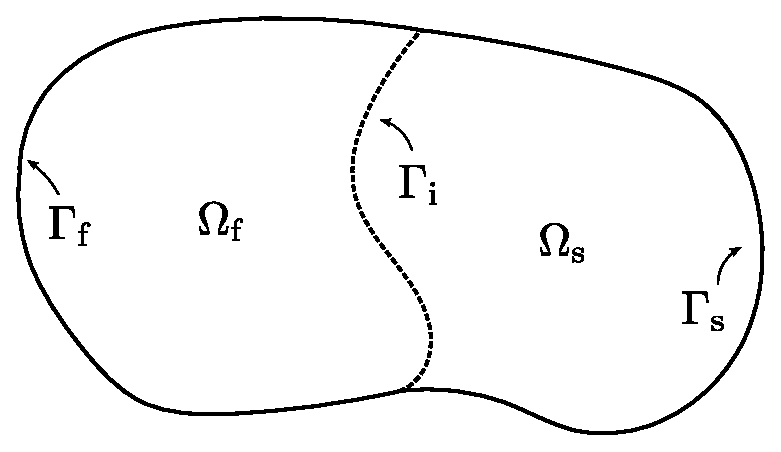
\includegraphics[scale=0.6]{Other_figures/Sketch_FSI.eps}
 	\caption {Sketch of a general FSI problem. } 
 	\label{fig:General-sketch-fsi-problem}
 \end{figure}  

\subsection{Governing equations\label{subsec:goerning_equations_FSI}}

Borrowing the notation developed in previous sections, we can expand it to account for a moving domain and to take into account the interaction between sub-domains. The FSI problem can be stated as: find a displacement $\boldsymbol{d}_{\mathrm{s}}$ in the solid problem, an associated velocity $\boldsymbol{u}_{\mathrm{s}} = \frac{\partial\boldsymbol{d}_{\mathrm{s}}}{\partial t}$,  and $\boldsymbol{U}=[\ufluid,\pfluid,\sigmafluid]$ for the standard formulation of the flow problem, or $\boldsymbol{U}=[\ufluid,\pfluid,\psifluid]$ for the LCR one, such that
\begin{align*}
    \rho_\mathrm{s}\left(\boldsymbol{d}_{\mathrm{s}}\right)\frac{\partial^{2}\boldsymbol{d}_{\mathrm{s}}}{\partial t^2} -\nabla \cdot \boldsymbol{\sigma}_{\mathrm{s}}\left(\boldsymbol{d}_{\mathrm{s}}\right) &= \rho_{\mathrm{s}}\left(\boldsymbol{d}_{\mathrm{s}}\right) \boldsymbol{b} && \text{ in } \ensuremath{\Omega}_{\rm{s}}(t), \; t\in]0,T[, \\ %\nonumber \\
    \boldsymbol{d}_{\mathrm{s}} &= \boldsymbol{d}_{\mathrm{s},D}  &&\text{ on } \Gamma_{\mathrm{s},D}(t), \; t\in]0,T[, \nonumber\\
    \boldsymbol{n}_\mathrm{s}\cdot\boldsymbol{\sigma}_\mathrm{s} &= \boldsymbol{t}_{\mathrm{s},N}  &&\text{ on } \Gamma_{\mathrm{s},N}(t), \; t\in]0,T[, \\ %\nonumber\\
    \boldsymbol{d}_{\mathrm{s}} &= \boldsymbol{d}_{\mathrm{s}}^0 &&\text{ in } \ensuremath{\Omega}_{\rm{s}}(0), \; t=0, \nonumber \\
    \boldsymbol{u}_{\mathrm{s}} &= \boldsymbol{u}_{\mathrm{s}}^0&&\text{ in } \ensuremath{\Omega}_{\rm{s}}(0), \; t=0, \\ 
    \mathcal{\mathcal{D}}_{t}\left(\boldsymbol{U}\right)+\mathcal{L}(\ufluid;\boldsymbol{U}) &= \boldsymbol{F} &&\text{ in } \ensuremath{\Omega}_{\rm{f}}(t), \; t\in]0,T[, \\ %\nonumber \\
    \ufluid&=\ufluidD  &&\text{ on }  \Gamma_{{\rm{f}},D}(t), \; t \in]0,T[,\nonumber \\
    \boldsymbol{n}_{\rm{f}}\cdot\sigmafluid&=\boldsymbol{t}_{{\rm{f}},N}  &&\text{ on }  \Gamma_{{\rm{f}},N}(t),  \; t \in]0,T[, \nonumber\\
    \ufluid&=\ufluid^0  &&\text{ in }  \Omega_{\rm{f}}(0), \; t=0, \\ %nonumber\\
    \sigmafluid&=\boldsymbol{\sigma}_{\rm{f}}^0  &&\text{ in }  \Omega_{\rm{f}}(0), \; t=0,  \\ %\nonumber \\
    \usolid &= \ufluid  &&\text{ on } \boundaryinterface(t), \; t \in]0,T[, \\ 
    \boldsymbol{t}_{\mathrm{s}} + \boldsymbol{t}_{\mathrm{f}}  & = {\bf 0},
    &&\text{ on } \boundaryinterface(t), \; t\in]0,T[,  %\label{eq_transmision_condition_tractions}.
 \end{align*}
where $\mathcal{\mathcal{D}}_{t},\mathcal{L} \text{ and } \boldsymbol{F}$ are identified depending upon the kind of formulation applied for the fluid, as seen in Section \ref{sec:Viscoelastic-fluid-flow-prob}, and  $\boldsymbol{t}_{\mathrm{s}}= -\boldsymbol{n}_{\mathrm{i}}\cdot\sigmasolid$. The last equations are known as the transmission conditions between sub-domains. In order to ensure accurate and stable dynamic simulations of FSI problems, dynamic and kinematic continuity must be guaranteed on the interaction interface. They are in charge of imposing same velocities and tractions on the interface boundary $\boundaryinterface(t)$. Let us recall that $\boldsymbol{t}_{\mathrm{f}}$ is computed according with the kind of formulation selected for the fluid as
\begin{equation*}
    \boldsymbol{t}_{\mathrm{f}}= \boldsymbol{n}_{\mathrm{i}} \cdot \sigmafluid 
\end{equation*}
for the standard formulation and 
\begin{equation*}
    \boldsymbol{t}_{\mathrm{f}}= \boldsymbol{n}_{\rm{i}}\cdot \dfrac{\eta_p}{\lambda_0}(\exp(\psifluid)-\boldsymbol{I})    
\end{equation*}
for the LCR.

The problem described has been written in the monolithic version, in which all unknowns are solved at once, in a fully coupled way. Coupling conditions are treated implicitly. 

\subsection{Block iterative scheme\label{subsec:iterative_scheme_FSI}}

Rather than solving the monolithic version of the problem, in this work a block-iterative coupling is considered, in which the solid and the fluid mechanics problems are solved sequentially. Strong coupling is considered; this is achieved by block-iterations that converge to the solution of the monolithic problem. This is essential to guarantee correct interface coupling as mesh displacements and velocities should be, up to a certain tolerance, equal, and continuity of tractions is also required. This coupling is of Dirichlet-Neumann type: the solid is solved with the loads computed from the fluid in a given iteration and then the fluid is computed with the velocities on the interface obtained from the solid (see below). 

Dynamic sub-relaxation is an efficient way to minimize the amount of sub-iterations necessary to achieve convergence. We have implemented an Aitken relaxation scheme, in particular Aitken $\Delta^2$, detailed in \cite{kuttler2008fixed}. Within each time step, let us denote by a superscript $k$ the $k$-th block-iteration of any variable. For clarity, let us omit the superscript with the time step counter. Suppose that from values at the $k$-th iteration, the solid is solved, obtaining the boundary velocities $\boldsymbol{u}_{{\Gamma_{\rm i},{\textrm{s}}}}^{k+1}$. Then, the fluid is solved from the boundary velocities $\boldsymbol{u}_{\Gamma_{\rm i}}^{k+1}$ computed as
\begin{align*}
\boldsymbol{u}_{\Gamma_{\rm i}}^{k+1} = \boldsymbol{u}_{\Gamma_{\rm i}}^{k} + \omega^{k+1} \boldsymbol{r}_{\Gamma_{\textrm{i}}}^{k+1},
\end{align*}
where
\begin{align*}
\boldsymbol{r}_{\Gamma_{\textrm{i}}}^{k+1} & := \boldsymbol{u}_{{\Gamma_{\rm i},{\textrm{s}}}}^{k+1}- \boldsymbol{u}_{\Gamma_{\rm i}}^{k},\quad
\omega^{k+1}  = -\omega^k \frac{(\boldsymbol{r}_{\Gamma_{\textrm{i}}}^{k})^{T}(\boldsymbol{r}_{\Gamma_{\textrm{i}}}^{k+1}-\boldsymbol{r}_{\Gamma_{\textrm{i}}}^{k})}{|\boldsymbol{r}_{\Gamma_{\textrm{i}}}^{k+1}-\boldsymbol{r}_{\Gamma_{\textrm{i}}}^{k}|^{2}}. 
\end{align*}
The algorithm is initialized taking a constant relaxation parameter (usually 0.1) in the two first coupling iterations. 

\begin{remark}
We have just considered a classical Aitken-accelerated partitioned approach to deal with the VFSI problem. Several new techniques have been developed over the last years to improve transmission conditions, such as quasi-Newton methods \cite{FSIQN2014,FSIQN2016}, domain decomposition techniques \cite{FSIDDM2015} or weak boundary transmission conditions \cite{FSIWeak2020}, which could also be applied to the current problem.
\end{remark}

\begin{remark}
In some works, it is recommended to apply relaxation of the displacement field instead of the velocity one. From our experience, the latter option is more convenient. If only the velocity field is relaxed, the interface between sub-domains from which the fluid solver computes tractions matches perfectly with the interface displacements. 
\end{remark}

Using the Dirichlet-Neumann iteration-by-subdomain coupling approach described earlier, the coupling algorithm to solve the problem is given in Algorithm~\ref{alg:algorithm1}.

\begin{algorithm}
\setlist{nosep}
\small
\caption{FSI algorithm}\label{alg:algorithm1}
%\begin{itemize}
$n = 0$; loop over the number of time steps.
\begin{itemize}
\item[] $n \gets n + 1$.
\item [] $k=0$; iterate until convergence.
\begin{itemize}
    \item[] $k \gets k + 1$ (block iteration counter omitted in the following).
 \item[$\bullet$] {\bf Solve the equations for the solid}, taking into account the tractions coming from the fluid problem $\boldsymbol{t}_{\mathrm{f}}$. At time $t^n$, omitting the superscript for the unknowns, these equations are:
 \begin{align*}
    \rho_\mathrm{s}\left(\boldsymbol{d}_{\mathrm{s}}\right)\frac{\delta_2^{2}\boldsymbol{d}_{\mathrm{s}}}{\delta t^2} -\nabla \cdot \boldsymbol{\sigma}_{\mathrm{s}}\left(\boldsymbol{d}_{\mathrm{s}}\right) &= \rho_{\mathrm{s}}\left(\boldsymbol{d}_{\mathrm{s}}\right) \boldsymbol{b} && \text{ in } \ensuremath{\Omega}_{\rm{s}}(t^n), \\
    \boldsymbol{d}_{\mathrm{s}} &= \boldsymbol{d}_{\mathrm{s},D}  &&\text{ on } \Gamma_{\mathrm{s},D}(t^n), \\
    \boldsymbol{n}_\mathrm{s}\cdot\boldsymbol{\sigma}_\mathrm{s} &= \boldsymbol{t}_{\mathrm{s},N}  &&\text{ on } \Gamma_{\mathrm{s},N}(t^n),\\
    \boldsymbol{n}_{\mathrm{i}} \cdot \sigmasolid &= \boldsymbol{t}_{\mathrm{f}} &&\text{ on } \boundaryinterface(t^n).
 \end{align*}
     \item[$\bullet$] {\bf Compute relaxed velocities} on the interface boundary $\boldsymbol{u}_{\boundaryinterface}$ with an Aitken relaxation scheme from the solid velocities
     $\boldsymbol{u}_{{\Gamma_{\rm i},{\textrm{s}}}} = \frac{\delta_2 \boldsymbol{d}_{\mathrm{s}}}{\delta t}\vert_{\Gamma_{\rm i}}$.
     \item[$\bullet$] {\bf Compute the domain velocity in the fluid} by solving the problem (see \cite{Mesh}):
    \begin{align*}
    -\nabla \cdot \left \lbrace \mathbb{C} \left(E_{\mathrm{dom}}\left( \boldsymbol{x}\right),\nu_{\mathrm{dom}} \right) : \nabla^{\rm s}\boldsymbol{u}_{\mathrm{dom}} \right \rbrace &={\bf 0} && \text{ in } \ensuremath{\Omega}_{\rm{f}}(t^n),\\
    \boldsymbol{u}_{\mathrm{dom}} &= \boldsymbol{u}_{\boundaryinterface}  &&\text{ on } \boundaryinterface(t^n), \\
    \boldsymbol{u}_{\mathrm{dom}} &= {\bf 0}  &&\text{ on } \Gamma_{{\rm{f}}}(t^n) \setminus \boundaryinterface(t^n),
  \end{align*}
    where $\mathbb{C}$ is the Constitutive 4th order tensor in linear elasticity, $E_{\mathrm{dom}}\left( \boldsymbol{x}\right)$ is the Young Modulus of the mesh computed at each node according to \cite{Mesh} and $\nu_{\mathrm{dom}} = 0.065$ is the Poisson coefficient of the mesh.
    \item[$\bullet$] {\bf Solve the ALE equations for the fluid}, taking into account the mesh velocity $\boldsymbol{u}_{\mathrm{dom}}$ and using the interface velocity $\boldsymbol{u}_{\boundaryinterface}$. If $\hat{\mathcal{D}}_t$ is a BDF2 approximation to ${\mathcal{D}}_{t}$, the equations to be solved at $t^n$ are:
    \begin{align*}
    \hat{\mathcal{D}}_{t}\left(\boldsymbol{U}\right)+\mathcal{L}(\ufluid;\boldsymbol{U}) &= \boldsymbol{F} &&\text{ in } \ensuremath{\Omega}_{\rm{f}}(t^n),\\
    \ufluid&=\ufluidD  &&\text{ on }  \Gamma_{{\rm{f}},D}(t^n),\\
    \boldsymbol{n}_{\rm{f}}\cdot\sigmafluid&=\boldsymbol{t}_{{\rm{f}},N}  &&\text{ on }  \Gamma_{{\rm{f}},N}(t^n), \\
    \ufluid &= \boldsymbol{u}_{\boundaryinterface},  &&\text{ on } \boundaryinterface(t^n).
 \end{align*}
 \item[$\bullet$] {\bf Check convergence and update unknowns}. When transmission conditions are satisfied on the interface boundary up to a tolerance, the coupling iterative loop ends.
\end{itemize}
\item[] End block-iterative loop.
\end{itemize}
End loop over the number of time steps.
%\end{itemize}
\label{FSI_algorithm}
\end{algorithm}



%%%%%%%%%%%%%%%%%%%%%%%%%%%%%%%%%%%%%%%
%
% NUMERICAL RESULTS
%
%%%%%%%%%%%%%%%%%%%%%%%%%%%%%%%%%%%%%%
\section{Numerical Examples\label{sec:numerical_examples}}

In this section, three numerical examples are presented to assess the performance of the proposed FSI solution strategy. In the first one, a flow through a channel with a flexible wall is considered to study the stationary solution. The main idea is to analyze the differences between the standard formulation and the logarithmic one when increasing the Weissenberg number of the problem. Next, so as to examine the effect of the viscosity, the well-known Turek's test \cite{turektest} is presented. In this case, the behavior of a laminar channel flow around an elastic object is studied when elasticity becomes dominant in the fluid. To end up, the influence of arterial mechanical properties in the blood flow in an aneurysm is analyzed. In particular the blood is modeled as a viscoelastic fluid.

Concerning the iterative scheme, for all examples a maximum of 15 iterations are set for both the fluid and the solid sub-problems, whose numerical relative tolerance in the $L^2$ norm is $10^{-5}$. Also, for the transmission conditions on the interface boundary (using again the $L^2$ norm), the relative tolerance is $10^{-3}$. In order to solve the monolithic system of linear equations for each sub-problem, we use the Biconjugate Gradients solver, \texttt{BiCGstab} \cite{BiconjugateGradientSolver}, which is implemented in the \texttt{PETSc} parallel solver library \cite{PETScHomePage}.

\textcolor{blue}{It is important to mention that mesh convergence results and their corresponding error estimation for the fluid side and the structural side are already performed in previous works. In the case of the standard three-field formulation for the viscoelastic fluid it can be found in \cite{castillo2014}. With respect to the LCR it is performed in detail in \cite{moreno2019logarithmic}. On the structural side, the classical displacement-based formulation for finite strain theory is considered. This formulation is widely used and its error analysis results are presented, for example, in \cite{Bonet}.} 

\subsection{Flow through a channel with a flexible wall\label{subsec:membrane}}

This first problem is a simplified test case of a flow in an elastic tube. This test is the standard one used by many authors as a reference benchmark for both Newtonian (for example \cite{luo1995numerical,luo1996numerical}) and shear-dependent non-Newtonian fluids (see \cite{lukavcova2008numerical,lukavcova2013kinematic}). Moreover, more recently, the works of Chakraborty et al. \cite{chakraborty2012fluid}  and Chen et al. \cite{Chen2014numerical} also consider viscoelastic fluids to explore new possible effects.
Essentially, the model consists of a steady flow in a channel where a part of the upper wall is replaced by an elastic plate. To sum up, firstly a study considering a Newtonian fluid will be performed, and later the effect of the viscoelasticity will be investigated, comparing the results with those that can be found in the literature. The benefits of the LCR approach proposed here will be highlighted.

\subsubsection{Set up}

The problem is defined according to the parameters proposed in \cite{Chen2014numerical,cai2003fluid}. The scheme of the domain can be observed in Fig. \ref{fig:FlexWall-scheme}. Regarding the channel measures, the rigid channel has height $D=0.01\ \rm{m}$. The flexible wall has a length of $5D$, located at $5D$ from the channel entrance. The length of the channel downstream of the flexible wall is $30D$.  For the computations, the flexible plate thickness $d$ varies between $0.01D$ and $0.1D$.

\begin{figure}[h]
    \centering
    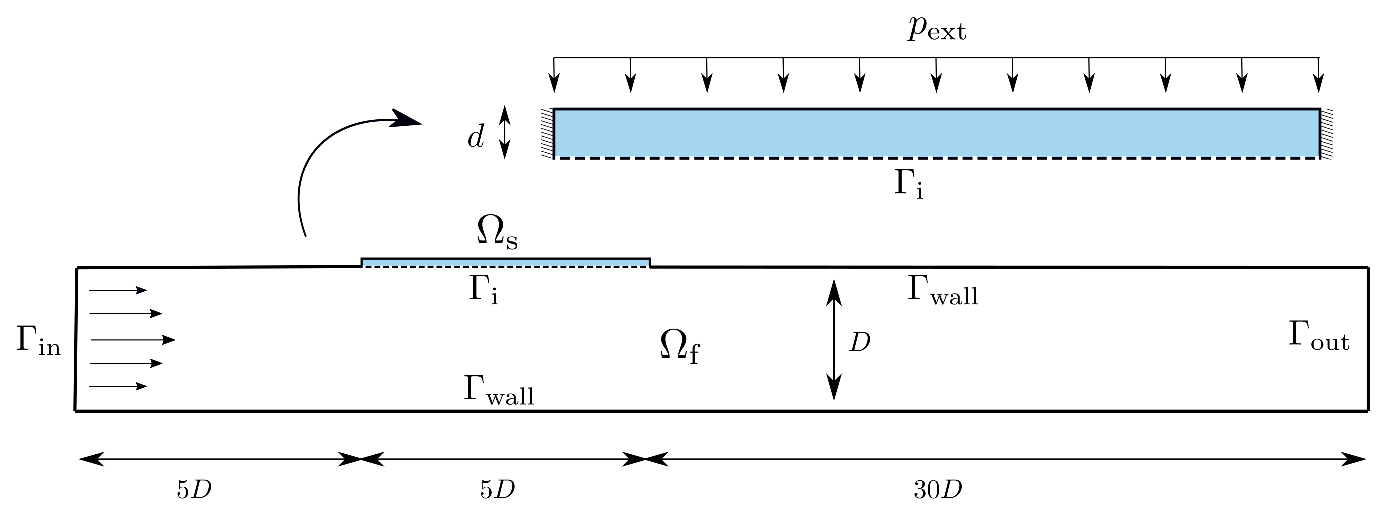
\includegraphics[scale=0.625]{Figures_Flexible_wall/Scheme_channel.eps}
    \caption{Flow through a channel with a flexible wall. Geometry.}
    \label{fig:FlexWall-scheme}
\end{figure}

Regarding the properties of the fluid,  the density is $\rho_{\rm{f}}=1\,000\ \rm{kg}/\rm{m}^3$ and the viscosity is $\eta=0.001\ \rm{Pa}\cdot \rm{s}$.  For the elastic plate the properties are as follows: an initial density $\rho_{\rm{s,0}}=1\,200\ \rm{kg}/\rm{m}^3$, a Young's modulus $E_{\mathrm{s}}=35.9\ \rm{kPa}$ and a Poisson's ratio $\nu_{\mathrm{s}}=0.45$. A Saint Venant-Kirchhoff material law is employed (see Subsection \ref{subsec:Saint-Venant-Kirchhoff} for a detailed description) and the plane strain assumption is considered.

Concerning the boundary conditions, in the inlet boundary of the fluid domain $\Gamma_{\rm{in}}$, a steady Poiseuille flow with average velocity $\bar{u}_\text{in}=0.03\ \rm{m}/\rm{s}$ is assumed; on the walls $\Gamma_{\rm{wall}}$ no-slip boundary conditions are imposed, and in the outlet $\Gamma_{\rm{out}}$ the pressure  is set to $p_{\rm{out}}=0$ Pa. A rectangular plate is considered as the solid domain, where an external pressure $p_{\rm{ext}}=1.755\ \rm{Pa}$ is distributed on the upper edge and it is clamped in both the left and the right sides. Therefore, the considered Reynolds number is ${\rm{Re}}=\rho_{\rm{f}} \bar{u}_{\rm in} D/\eta=300$, where $\bar{u}_{\rm in}$ is the average inlet velocity in the channel direction.

The domains are discretized by using bilinear structured elements ($Q_1$). Two meshes have been used for this example, whose numbers of  elements are summarized in Table \ref{tab:FlexWal-Meshes}. The meshes M1f and M1s are employed for the Newtonian fluid flow study, and finer meshes M2f and M2s are used for studying all the viscoelastic cases.

\begin{table}[h]
    \begin{centering}
        \begin{tabular}{crcr}
            \toprule 
            \textbf{Fluid mesh}  & \textbf{Elements} & \textbf{Solid mesh}  & \textbf{Elements} \tabularnewline
            \toprule
            M1f  & 3\,000 & M1s  &   600  \tabularnewline
            M2f  & 10\,500 & M2s  &  1\,500 \tabularnewline
            \bottomrule 
        \end{tabular}
    \par\end{centering}
    \caption{Flow through a channel with a flexible wall. Main characteristics of the computational meshes.}
    \label{tab:FlexWal-Meshes}
\end{table}

\subsubsection{FSI problem using a Newtonian fluid}

Firstly, the validation considering a Newtonian regime is performed. For that, six different thickness have been considered to see the effect on the plate deformation. The distribution of velocities, pressures and stresses in the channel can be seen in Fig.~\ref{fig:FlexWal-field-distributions}. Note that the solution fields are similar for all six cases and, for this reason only one case is shown here. In these pictures, only the part of the domain where the plate is located has been plotted. The maximum velocity is reached in the narrowing of the channel produced by the deformed wall. Also, a peak of pressure and stress is observed in this area as a consequence of the local reduction of the channel width.

\begin{figure}[h!]
    \centering
    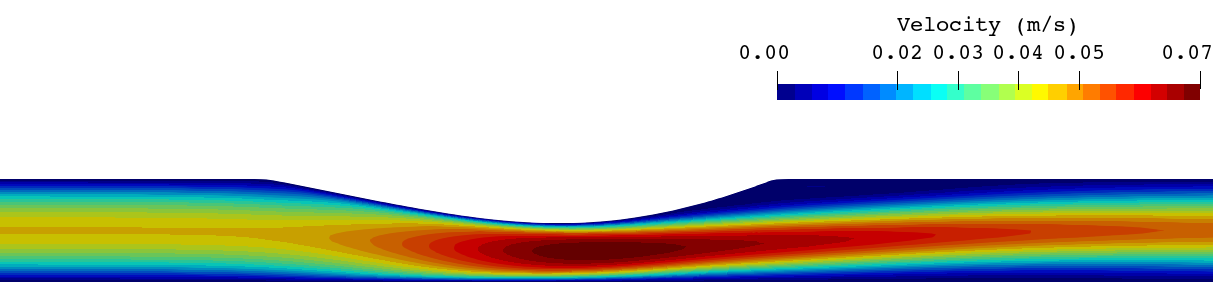
\includegraphics[scale=0.35]{Figures_Flexible_wall/Distribution_velocity.png}
    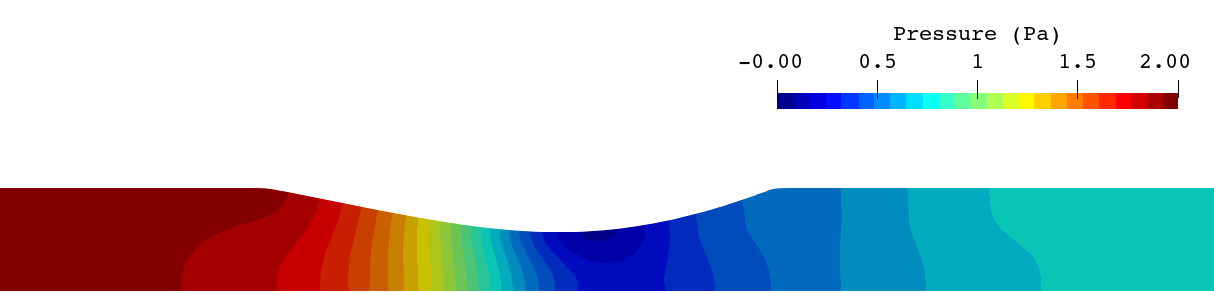
\includegraphics[scale=0.35]{Figures_Flexible_wall/Distribution_press.png}
    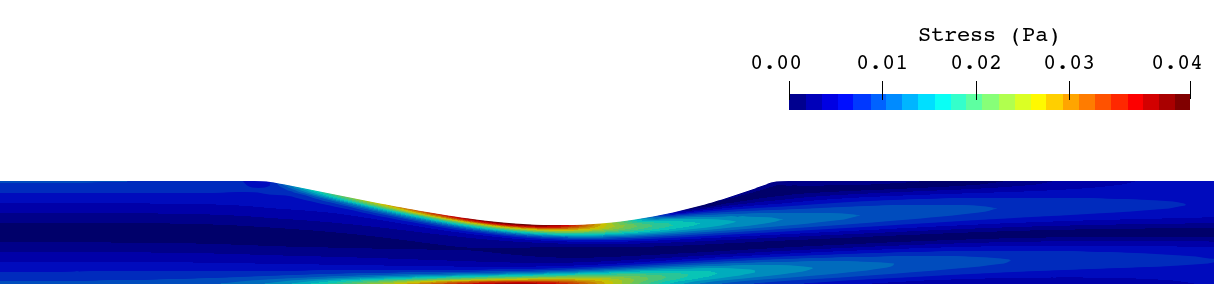
\includegraphics[scale=0.35]{Figures_Flexible_wall/Distribution_stress.png}
    \caption{Flow through a channel with a flexible wall. Distribution of the velocity field (top), pressure (middle) and the stresses (bottom) in the fluid domain around the plate location for the plate thickness $d=0.01D$. Velocities and stresses are plotted using their Euclidean norm.}
    \label{fig:FlexWal-field-distributions}
\end{figure}
\begin{figure}[h!]
    \centering
    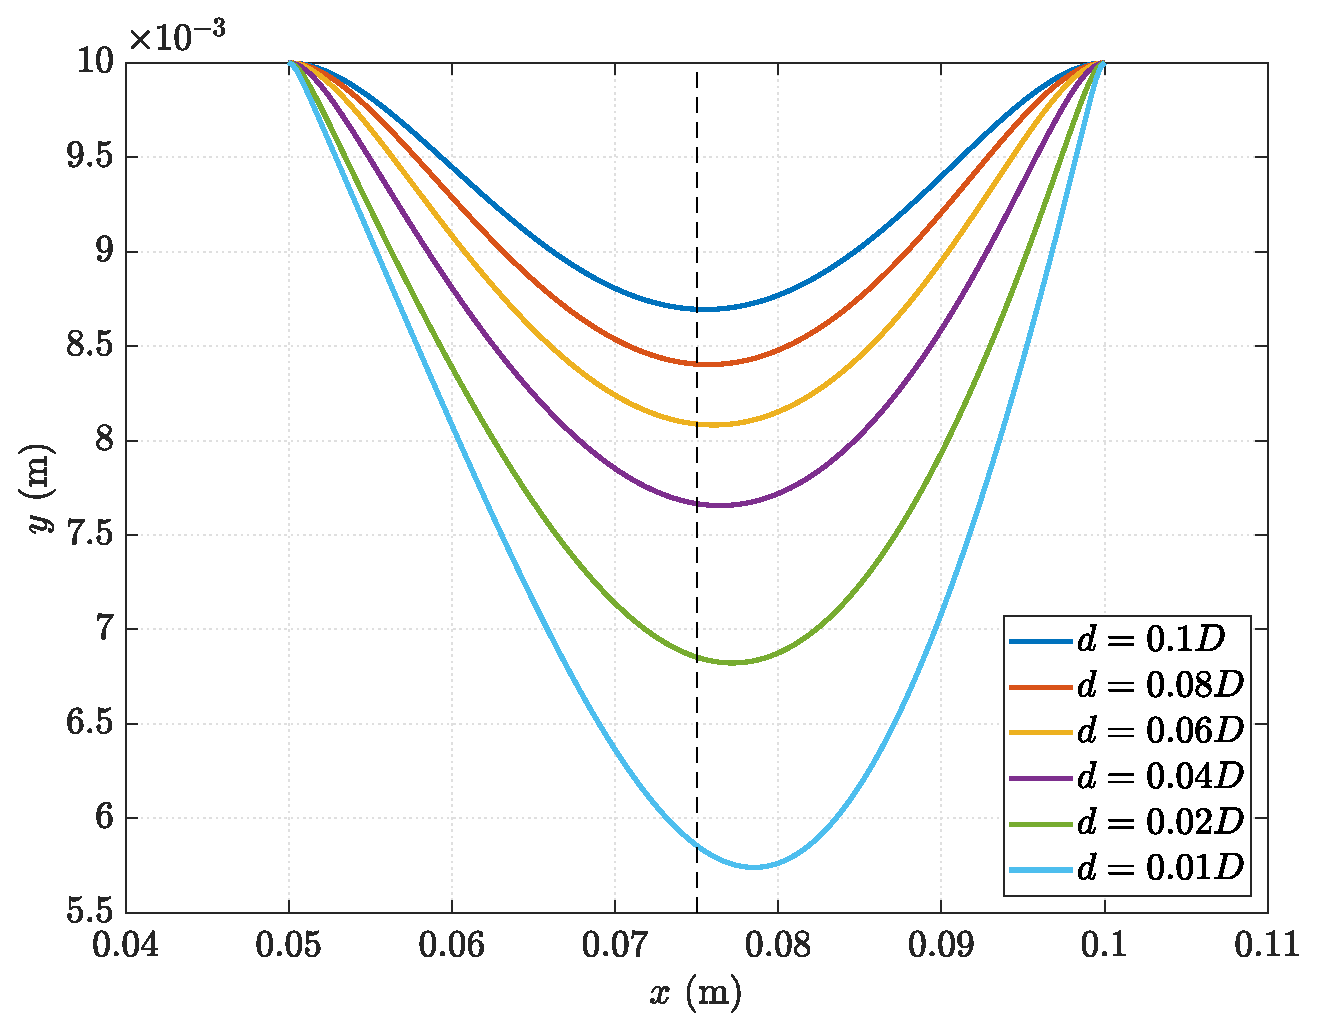
\includegraphics[scale=0.5]{Figures_Flexible_wall/Newtonian_deformation.eps}
    \caption{Flow through a channel with a flexible wall. Comparison of the vertical displacement of the plate for different thicknesses $d$ using a Newtonian fluid.}
    \label{fig:FlexWal-newtonian-comparison}
\end{figure}

The vertical displacement of the flexible plate for different thicknesses, from $d=0.1D$ to $d=0.01D$, can be observed in Fig.~\ref{fig:FlexWal-newtonian-comparison}. As expected, the thickest plate is the less deformed one. The effect reported is that the slenderer the plate is, the higher the deformation of the plate becomes.  Moreover, as the thickness increases, the lowest point of the wall moves upwards gradually due to the increment of forces exerted by the fluid. These results are in agreement with those reported in \cite{Luo2007} and \cite{Chen2014numerical}.

\subsubsection{FSI problem using a viscoelastic fluid}

Once the Newtonian fluids have been tested, the study of the deformation for the thinnest plate (of thickness $d=0.01D$) is carried out, but now varying the elasticity of the fluid. In other words, the problem using a viscoelastic fluid for several Weissenberg numbers is computed, so as to study the evolution of the flow when elasticity becomes dominant. The physical parameters have been set as in the previous section, with the exception of the relaxation time of the fluid and the $\beta$ parameter, that now is set to 0.5.

\begin{figure}[h!]
    \centering
    \subfloat[]{
    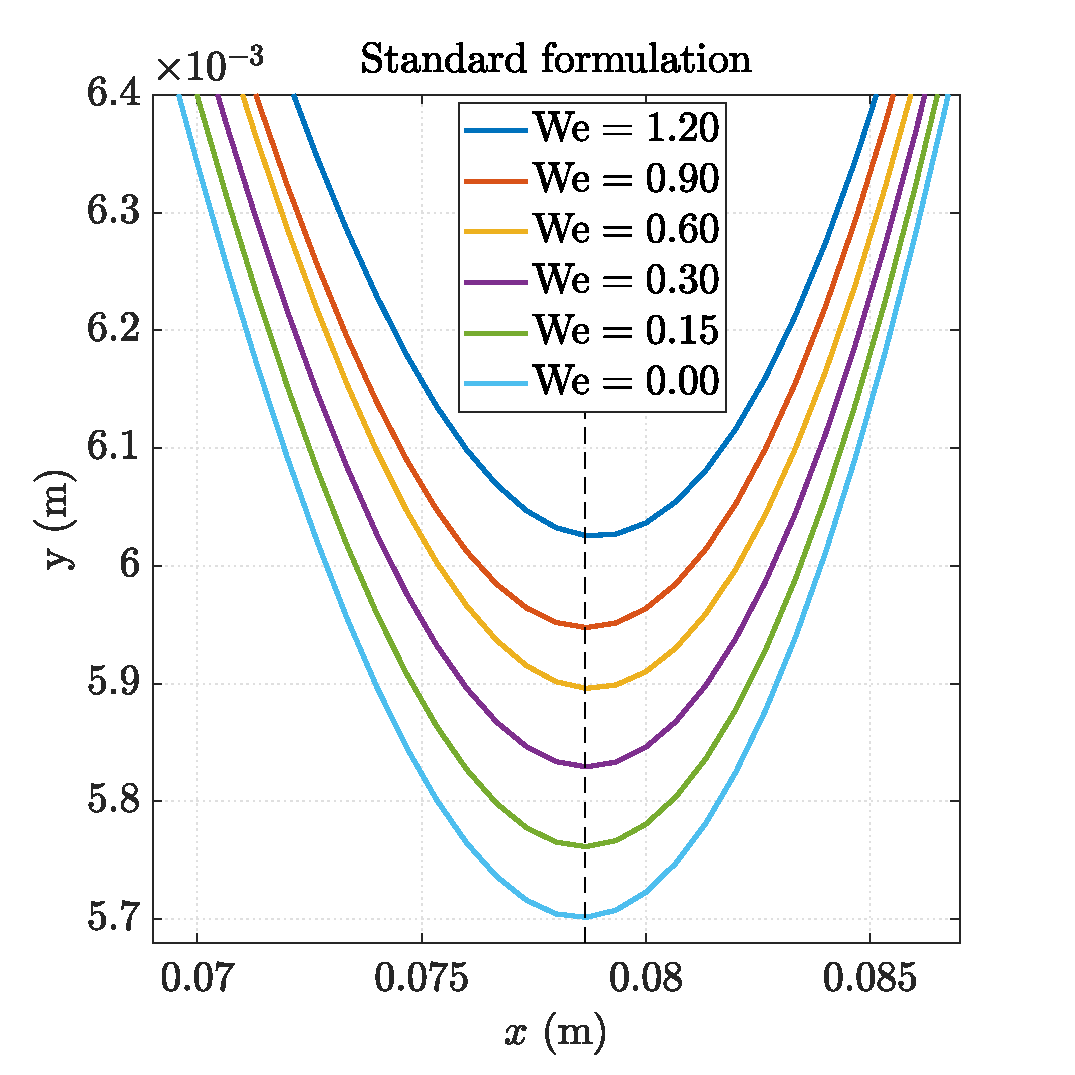
\includegraphics[scale=0.425]{Figures_Flexible_wall/Standard.eps}}
    \subfloat[]{
    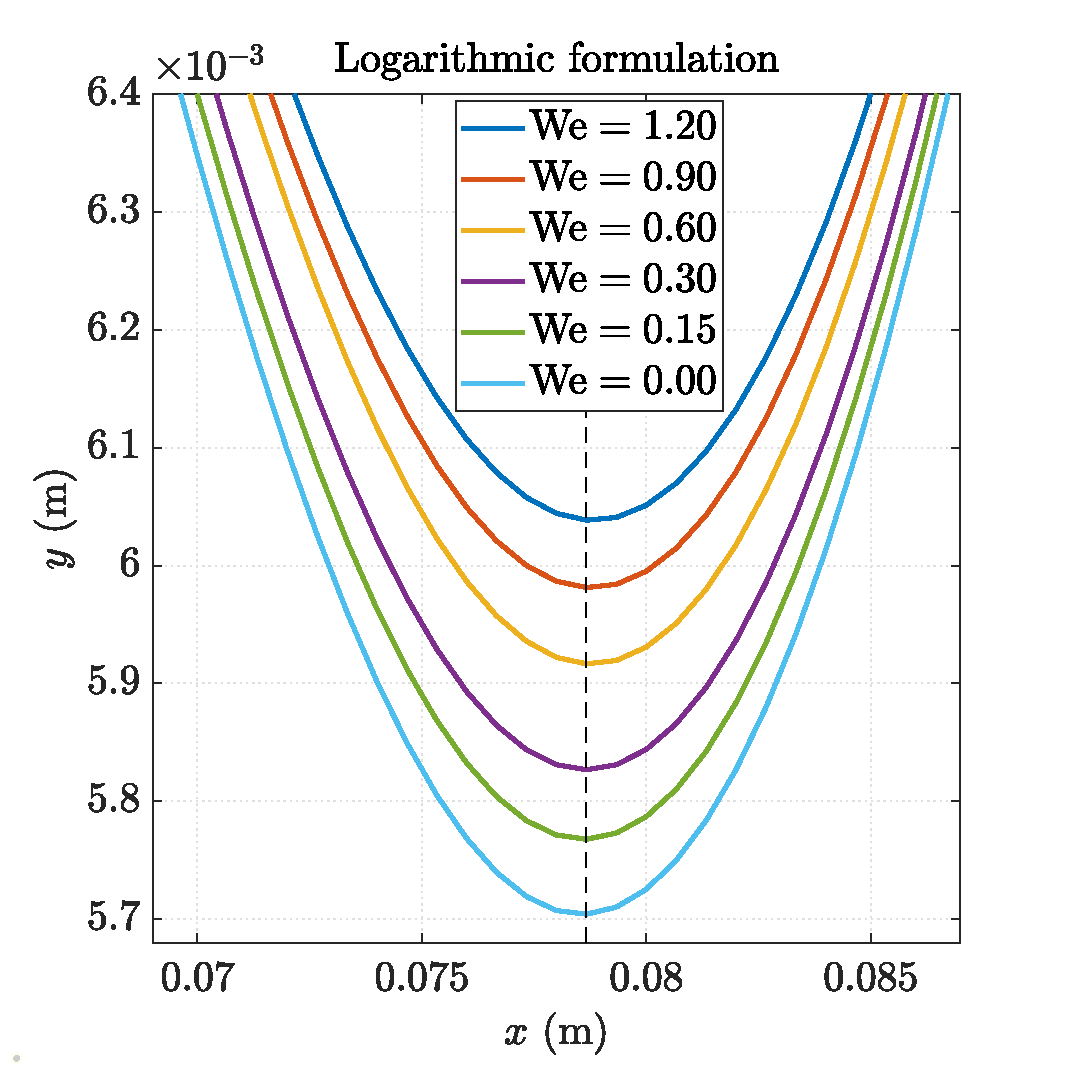
\includegraphics[scale=0.425]{Figures_Flexible_wall/Logarithmic.eps}}
    \caption{Flow through a channel with a flexible wall. Comparison of the deformation of the plate with thickness $d=0.01D$ for several We numbers.}
    \label{fig:FlexWall-We-displacement-comparison}
\end{figure}

Firstly, the deformation changes in the plate will be explored when the Weissenberg number increases, by using both fluid formulations (standard and LCR). This study is plotted in Fig.~\ref{fig:FlexWall-We-displacement-comparison}, where the deformation of the plate in each case is drawn from $\rm{We}=0$ to $\rm{We}=1.2$, which corresponds to relaxation times from $\lambda=0$ s to $\lambda=0.4$ s, respectively. Note that the results with $\text{We}=0$ correspond exactly with the Newtonian fluid behavior. The classical Navier-Stokes equations written in a three-field formulation setting are automatically recovered. 

It is interesting to highlight the phenomena produced when the elasticity becomes dominant. An attenuation of the deformation in the plate is produced. This effect is also reported in \cite{Chen2014numerical}, and it is explained by the presence of a higher elasticity in the fluid: when elasticity increases, stresses do so significantly. 

So as to clarify this physical effect, Table \ref{tab:FSI1 Forces} shows a summary of the fluid forces on the solid and the momentum with respect to the center of gravity of the flexible wall. The external pressure $p_{\rm{ext}}$ acting over the plate causes a vertical force equal to $0.8775\cdot10^{-1}\text{ N}$. As it can be observed in Table~\ref{tab:FSI1 Forces}, the resulting vertical fluid force increases as We increases. That force is acting in the opposite direction to the one coming from the external pressure, reducing the deflection of the plate. It is important to mention that a small movement upwards is also appreciated in the lowest point of the wall in Fig. \ref{fig:FlexWall-We-displacement-comparison}. Clearly it is caused by the reduction of momentum at the center of gravity of the membrane.

\begin{table}[h!]
    \begin{centering}
        \begin{tabular}{lcccc}
            %\toprule 
            \hline
            \textbf{We}  & \textbf{x-force} [$10^{-2}$ \textbf{N}] & \textbf{y-force} [$10^{-1}$ \textbf{N}] & \textbf{Momentum} [$10^{-2}$ \textbf{N·m}] \tabularnewline
            %\toprule
            \hline
            0.0  & 0.6225 & 0.4018 & $-0.3704$ \tabularnewline
            0.15 & 0.6056 & 0.4130 & $-0.3545$\tabularnewline
            0.3  & 0.6098 & 0.4399 & $-0.3389$ \tabularnewline
            0.6  & 0.5734 & 0.4554 & $-0.3344$ \tabularnewline
            0.9  & 0.5416 & 0.4754 & $-0.3155$\tabularnewline
            1.2  & 0.5534 & 0.5186 & $-0.3085$\tabularnewline
            \hline
        \end{tabular}
    \par\end{centering}
    \caption{Flow through a channel with a flexible wall. Horizontal and vertical forces and momentum with respect to the solid center of gravity.}
    \label{tab:FSI1 Forces}
\end{table}

Both formulations (standard and LCR) show similar results for the plate displacement, although slight differences can be reported for $\rm{We}$ up to 0.3. These are explained by the different treatment of the stresses. However, when the element size is small enough, the solution converges exactly to the same solution, independently of the employed formulation.

Furthermore, we also study the distribution of pressure and first component of stress in the flexible wall for each computed case, plotted in Fig. \ref{fig:FlexWall-viscoelastic-comparison}. We have displayed the component $\sigma_{xx}$ instead of the others because it is the most characteristic component of the stress tensor in this location. As expected, both solutions become higher when the elasticity of the fluid increases.

\begin{figure}[h!]
    \centering
    \subfloat[]{
    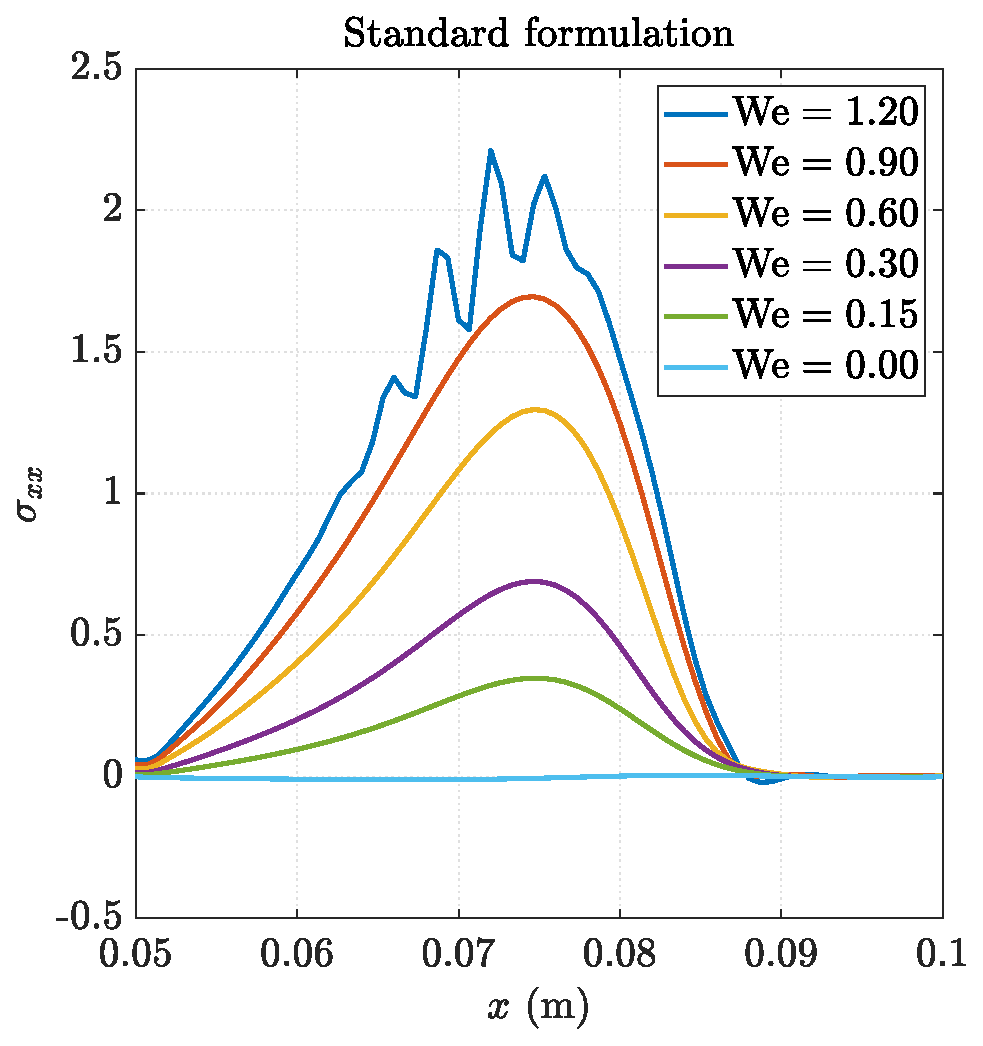
\includegraphics[scale=0.41]{Figures_Flexible_wall/Viscoelastic_stressxx_std.eps} \label{fig:FlexWall-stress-std}}
    \subfloat[]{
    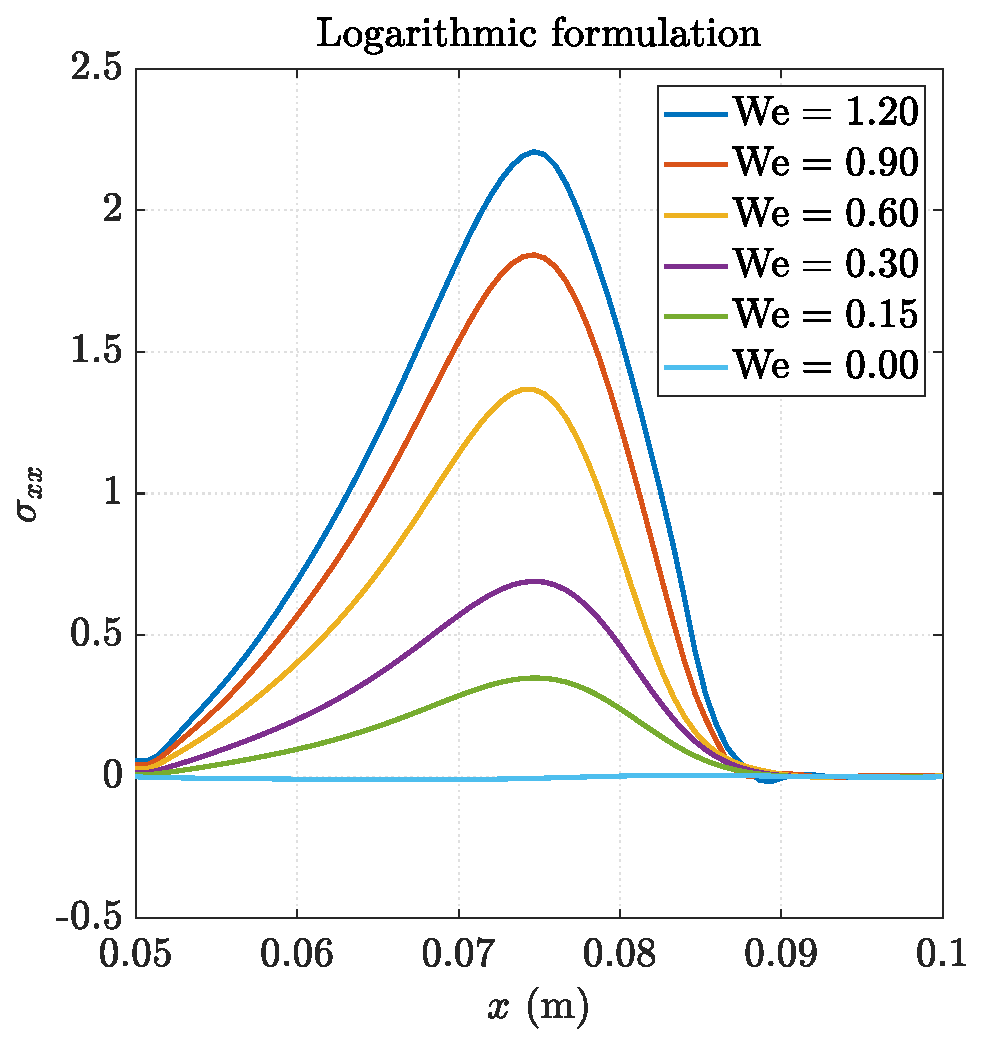
\includegraphics[scale=0.41]{Figures_Flexible_wall/Viscoelastic_stressxx_log.eps} \label{fig:FlexWall-stress-log}}\\
    \subfloat[]{
    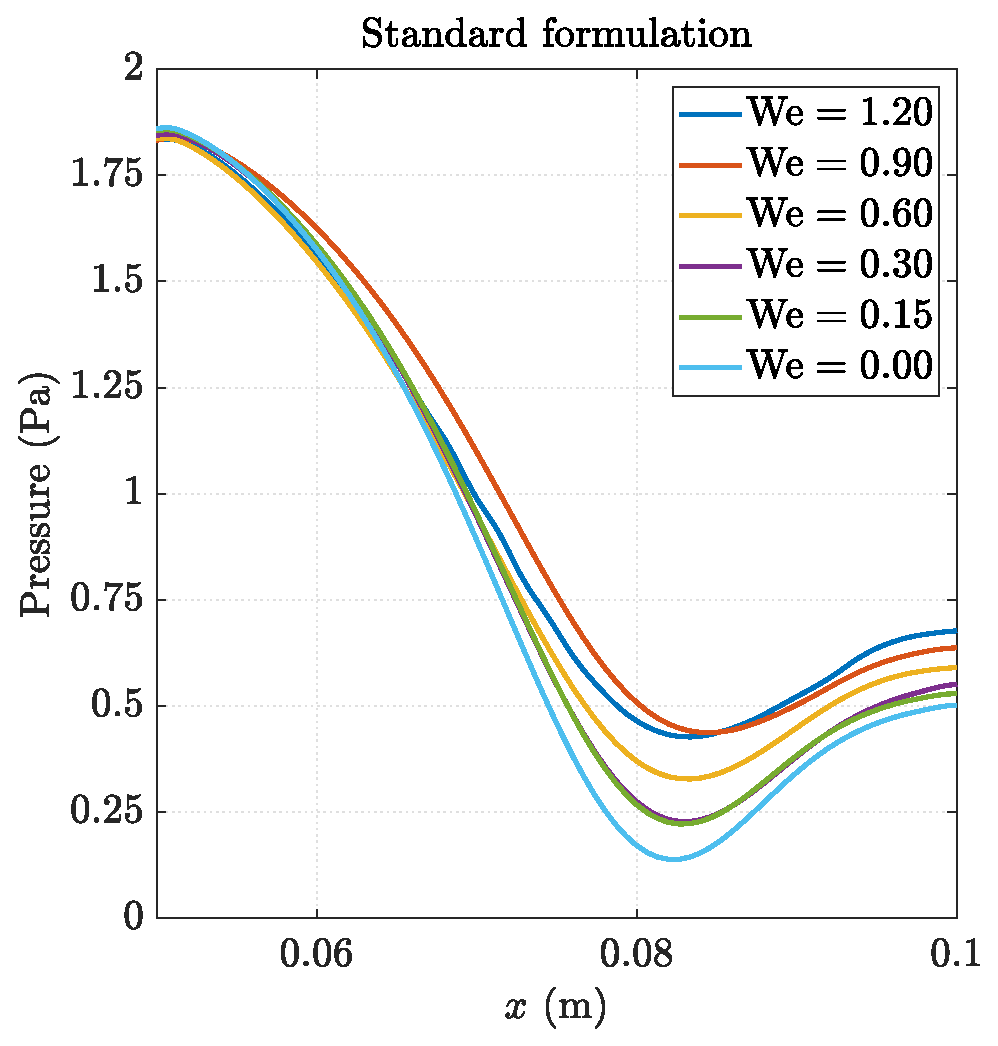
\includegraphics[scale=0.41]{Figures_Flexible_wall/Viscoelastic_pressure_std.eps}
    \label{fig:FlexWall-pressure-std}}
    \subfloat[]{
    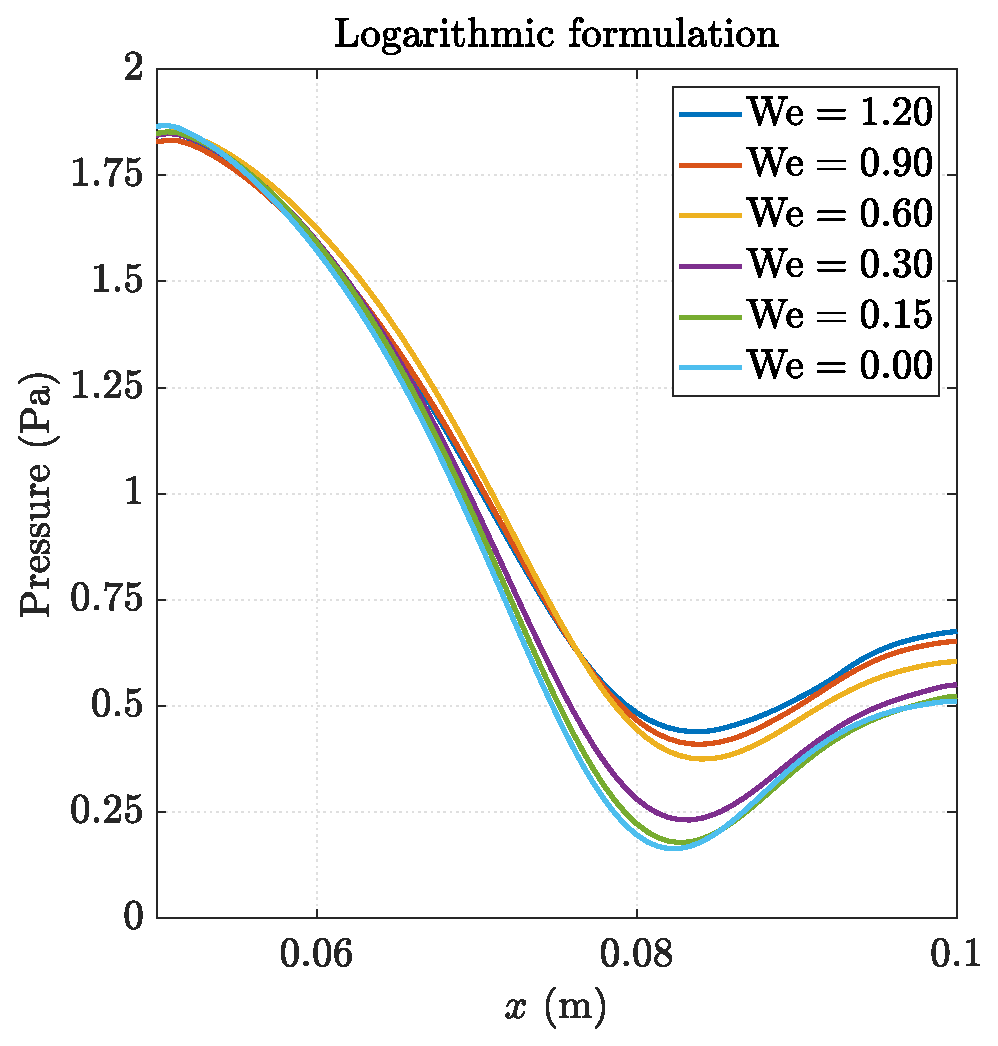
\includegraphics[scale=0.41]{Figures_Flexible_wall/Viscoelastic_pressure_log.eps}
    \label{fig:FlexWall-pressure-log}}
    \caption{Flow through a channel with a flexible wall. Comparison of the first component of stress and pressure in the plate with thickness $d=0.01D$ using the standard and the LCR formulation.}
    \label{fig:FlexWall-viscoelastic-comparison}
\end{figure}

First of all, let us remark that for the highest elastic case computed ($\rm{We}=1.2$), results do not show a smooth solution for stresses when the standard formulation is employed, probably due to a lack of mesh resolution in this location; this can be clearly seen in Fig. \ref{fig:FlexWall-stress-std}. This non-smoothness is also reported in \cite{Chen2014numerical}, in which the smooth solution is reached using finer meshes.
{Note that this area presents large stress gradients, regions with particularly high deformation rate, and therefore this location is highly sensitive to  the instability caused by the HWNP.  However, through the application of the LCR approach, able to deal with the instability, a regular solution can be obtained, as it can be observed in Fig.~\ref{fig:FlexWall-stress-log}.}

For We numbers up to 0.3, the LCR is able to capture higher values for the peaks of stresses than the standard formulation; concerning the pressure field, a bad solution is obtained for $\rm{We}=1.2$ for the standard formulation, as it can be observed in Fig.~\ref{fig:FlexWall-pressure-std}. Despite the fact of obtaining a smooth solution, it should be higher than the one obtained for $\rm{We}=0.9$. A correct solution is obtained if the LCR for the viscoelastic fluid is used, as it is shown in Fig.~\ref{fig:FlexWall-pressure-log}. 

All the cases reported until $\rm{We}=1.2$ have a converged solution using both formulations. It is important to remark that the employed formulation does not affect significantly the final displacement of the plate, even for the fluid flow with high Weissenberg number, as it can be seen in Fig.  \ref{fig:FlexWall-We-displacement-comparison}. However, the iterative scheme suffers a breakdown for the standard formulation when $\text{We} > 1.2$. This breakdown seems to be caused by the incapability of the formulation of capturing suitably both the stress and the pressure fields for the chosen mesh with $\rm{We}=1.2$ (see Fig. \ref{fig:FlexWall-viscoelastic-comparison}).

\subsection{Turek's test\label{subsec:turek}}

In this case, we study the FSI between an hyperelastic structure and a laminar flow. This benchmark is used by many authors as a reference test to check their implementations of the FSI problem  \cite{turektest}. The configuration consists of a laminar channel flow around an elastic object which results in self-induced oscillations of the structure.  Firstly, a study considering a Newtonian fluid will be performed and compared with the literature, and then the effect of the viscoelasticity will be investigated.

\subsubsection{Setup}

The geometry of the problem  is displayed in Fig. \ref{fig:turek_geometry}. The rigid channel has height $H = 0.41$ m and length $L=2.5$ m. The circle center is positioned at point $C = (0.2,0.2)$ m (measured from the left bottom corner of the channel) and its radius is $r = 0.05$ m. The structure bar has length $l = 0.35$~m and height $h = 0.02$~m. The right bottom corner is positioned at $(0.6,0.19)$ m, and the left end is fully attached to the fixed cylinder.



\begin{figure}[h!]
    \centering
    %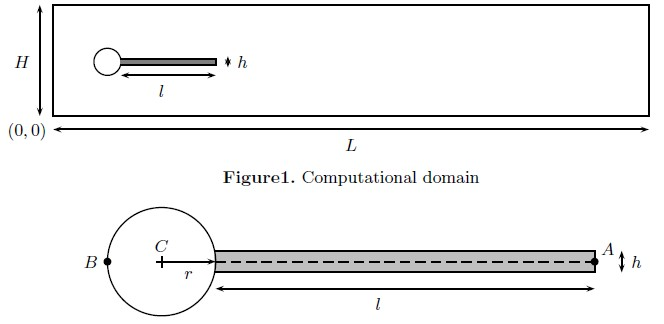
\includegraphics[scale=0.4]{Figures_Turek/turek_geometry.jpg}
    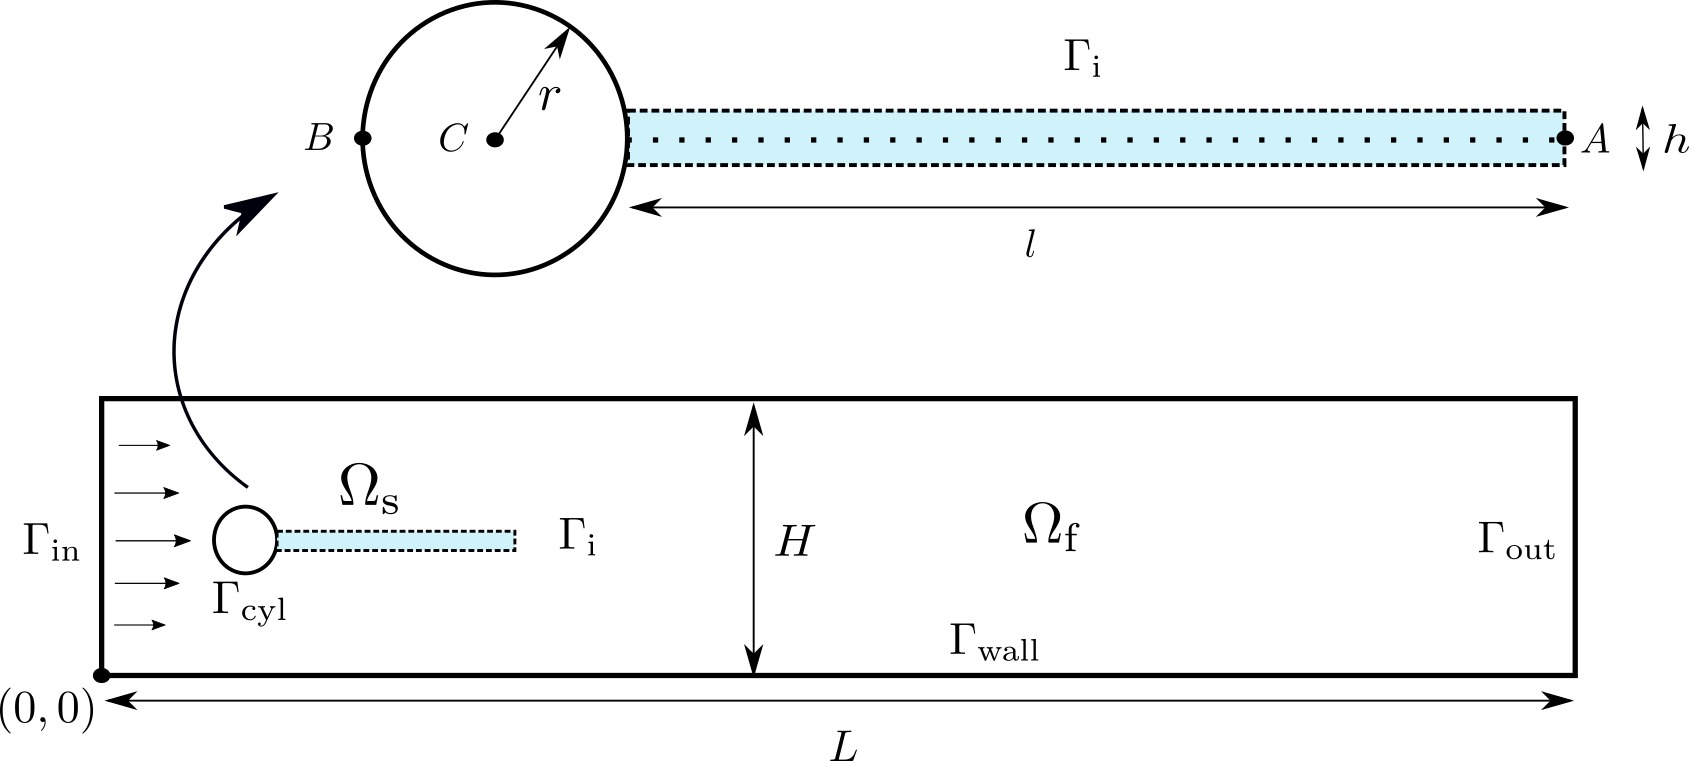
\includegraphics[scale=0.8]{Figures_Turek/Turek_scheme.png}
    \caption{Turek's test. Geometry.}
    \label{fig:turek_geometry}
\end{figure}

With regards to boundary conditions, a parabolic profile is prescribed at the left channel inflow, given by
\begin{equation}
    \bar{u}_{\rm{f}} (0,y) = 1.5 \, \bar{u}_{\rm in} \frac{y ( H - y )}{\left ( \frac{H}{2} \right )^2},
\end{equation}
such that the mean inflow velocity is $ \bar{u}_{\rm in}$ and the maximum of the inflow velocity profile is $1.5 \bar{u}_{\rm in}$.  A smooth increase of the velocity profile in time is prescribed, given by
\begin{equation}
    {u}_{\rm{f}} (0,y,t)=\begin{cases}
    \bar{u}_{\rm{f}} (0,y)\frac{1-\cos{\frac{\pi}{2}t}}{2} & t < 2.0\text{ s}\\
    {u}_{\rm{f}} (0,y) & \text{otherwise}
    \end{cases}. \label{eq:initial_condition_parabolic_profile}
\end{equation}
The outflow condition is considered stress free. Finally, a no-slip condition is prescribed for the fluid on the other boundary parts. 
Concerning the boundary conditions of the structure, fixed null displacement is considered in the left edge.

Two FSI tests are performed: on the one hand, FSI1, which results in a stationary solution; on the other hand, FSI2, which has a periodic solution. Table \ref{fig:turek_parameter_settings} shows the parameter settings for each FSI case. Note that here the viscosity of the fluid is the kinematic one.

\begin{table}[h]
    \begin{center}
        \begin{tabular}{lrr}
            \toprule
            \textbf{Parameter}                                           & \textbf{FSI1} & \textbf{FSI2}  \tabularnewline
            \toprule
            $\rho_\mathrm{s,0}$ {[}$10^3 \frac{\text{kg}}{\text{m}^3}${]}  & 1 & 10            \tabularnewline
            $\nu_{\mathrm{s}}$ {[-}{]}                                   & 0.4 & 0.4         \tabularnewline
            $E_\mathrm{s}$ {[}$10^6 \frac{\text{kg}}{\text{ms}^2}${]}    & 1.4 & 1.4         \tabularnewline 
            \toprule
            $\rho_\mathrm{f}$ {[}$10^3 \frac{\text{kg}}{\text{m}^3}${]}  & 1 & 1             \tabularnewline
            $\nu_{\mathrm{f}}$ {[}$10^{-3}\frac{\text{m}^2}{\text{s}}${]}& 1 & 1             \tabularnewline
            $ \bar{u}_{\rm in}$ {[}$\frac{\text{m}}{\text{s}}${]}            & 0.2 & 1           \tabularnewline
            Re [-]                                                          & 20 & 100          \tabularnewline
            \bottomrule
        \end{tabular}
        \caption{Turek's test. Parameter settings for the FSI1 and FSI2 cases.}
        \label{fig:turek_parameter_settings}
    \end{center}
\end{table}

The domains are discretized using $P_1$ (linear) elements for the fluid domain and $Q_1$ (bilinear) elements for the solid one. Regarding the distribution of the elements, the mesh is finer around the cylinder and the bar, while downstream the mesh is coarser, as it can be observed in Fig.~\ref{fig:Turek-mesh-employed}. In total, the fluid mesh is formed by 25\,000 unstructured elements, and the solid mesh by 10\,000 (20 $\times$ 500) structured elements.

\begin{figure}[h!]
    \centering
    \subfloat[Mesh of the fluid domain]{
    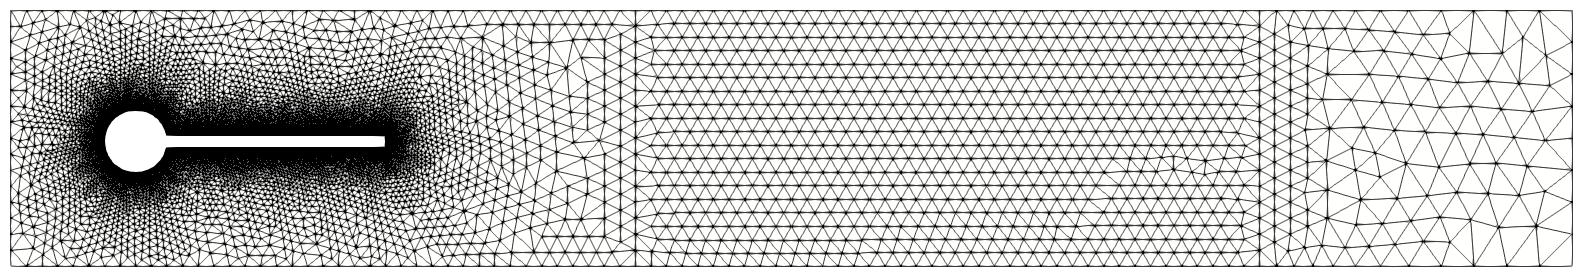
\includegraphics[scale=0.22]{Figures_Turek/Mesh_Fluid.png} \label{}}\\
    \subfloat[Zoom around the cylinder and bar and mesh of the solid domain]{
    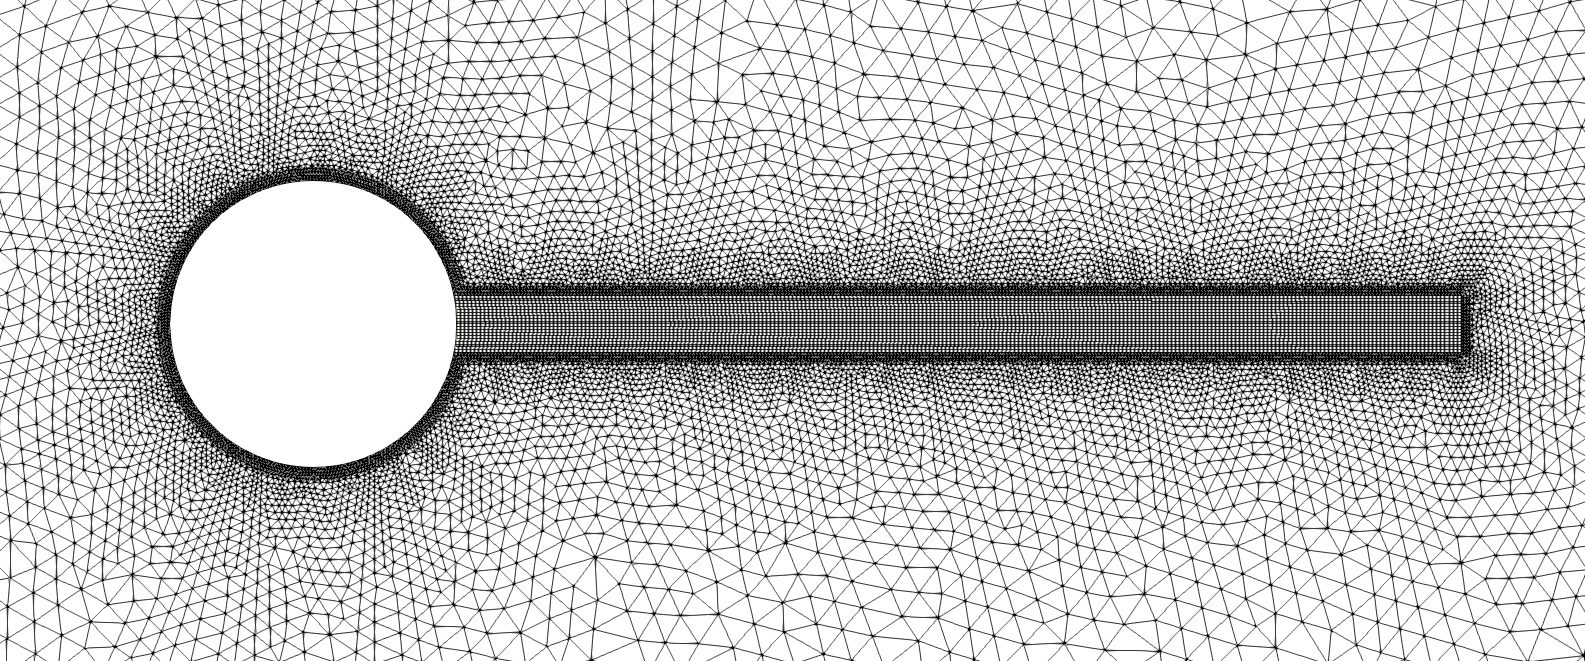
\includegraphics[scale=0.22]{Figures_Turek/Zoom_mesh.png} \label{}}
    \caption{Turek's test. Mesh domain.}
    \label{fig:Turek-mesh-employed}
\end{figure}

\subsubsection{FSI problem using a Newtonian fluid}

The aim of this section is to compare our results with the ones coming from the benchmark in~\cite{turektest} by using a Newtonian fluid and a Saint Venant-Kirchhoff solid material. First of all, the stationary case FSI1 is validated with reference \cite{turektest} in Table \ref{tab:FSI1_Newtonian_Results}, which includes displacements, drag and lift forces. The results completely agree with the reference ones, as it can be observed. For these computations the LCR formulation have been employed, but note that the solution would be exactly the same for the standard one due to for $\rm{We}=0$ (and therefore $\lambda=0$) we recover exactly the Navier Stokes equations written in a three-field setting.

\begin{table}[h]
    \begin{centering}
        \begin{tabular}{ccccc}
            %\toprule 
            \hline
             & \textbf{x-disp of A [$10^{-4}$ m]} & \textbf{y-disp of A[$10^{-3}$ m]}  & \textbf{drag} [N] & \textbf{lift} [N]  \tabularnewline
            %\toprule
            \hline
            Current paper& 0.2241 & 0.8202 & 14.263 & 0.7657 \tabularnewline
            Reference \cite{turektest} & 0.2270 & 0.8209 & 14.295 & 0.7638 \tabularnewline
            %\bottomrule 
            \hline
        \end{tabular}
    \par\end{centering}
    \caption{Turek's test. Displacement at point A and forces exerted by the fluid on the whole submerged body (cylinder and beam) for FSI1 benchmark.}
    \label{tab:FSI1_Newtonian_Results}
\end{table}

Moreover, the dynamic case is also tested, namely FSI2. Fig. \ref{fig:Turek-different-times} shows the solution for three different times. The bar displacements observed and the lift and drag obtained are also in agreement with the reference paper. We can conclude that the FSI algorithm has been suitably checked.

\begin{figure}[h!]
    \centering
    \subfloat[$t=34.0$]{
    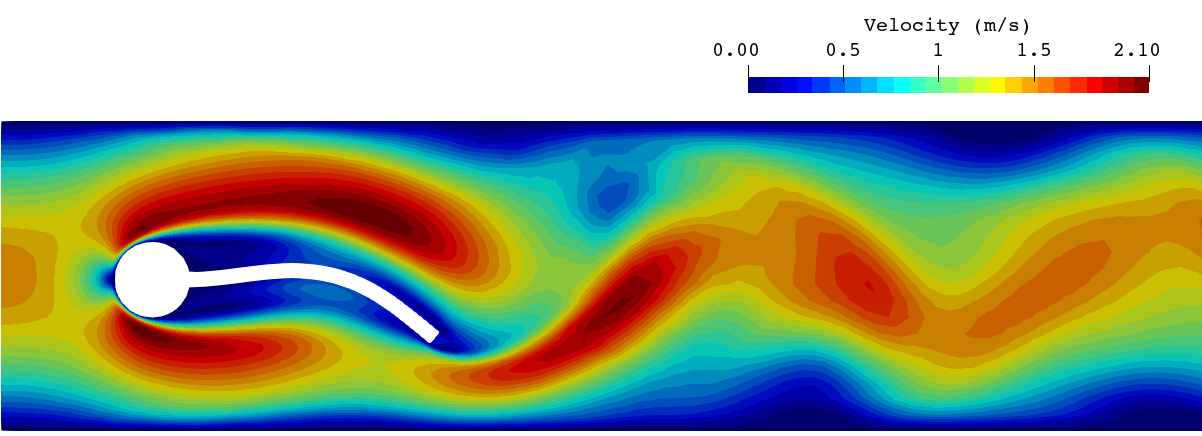
\includegraphics[scale=0.25]{Figures_Turek/101.png} \label{}}\\
    \subfloat[$t=34.1$]{
    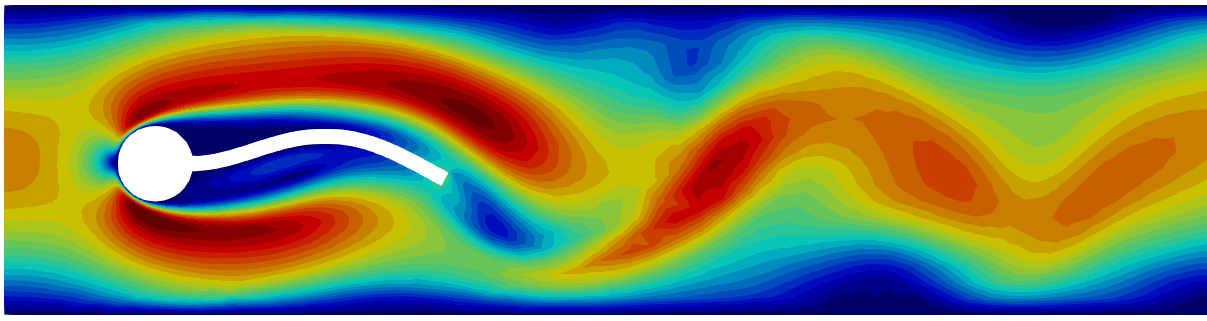
\includegraphics[scale=0.25]{Figures_Turek/102.png} \label{}}\\
    \subfloat[$t=34.3$]{
    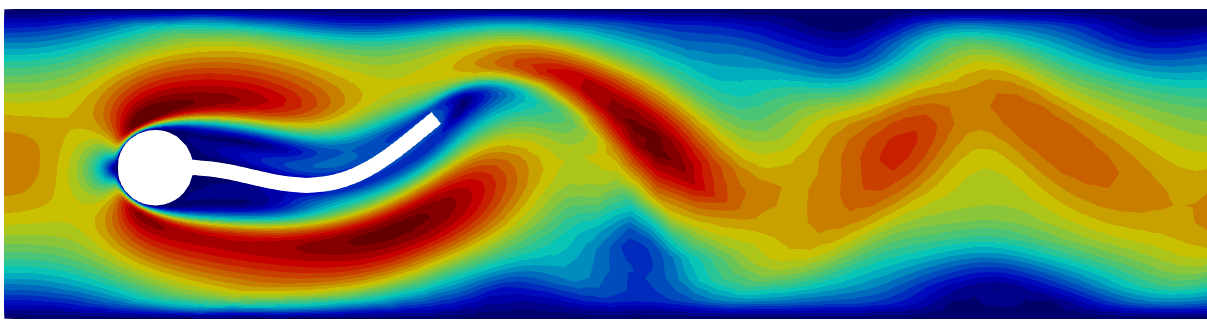
\includegraphics[scale=0.25]{Figures_Turek/104.png}}\\
    %\subfloat[$t=10.5$]{
    %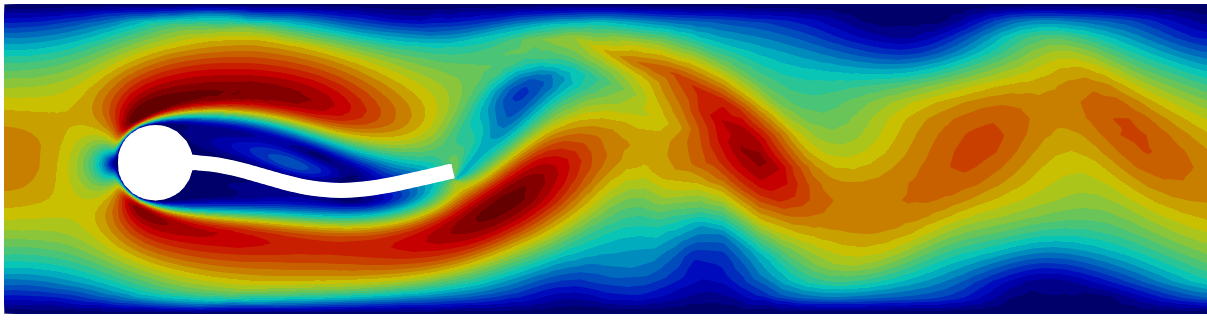
\includegraphics[scale=0.25]{Figures_Turek/105.png}}
    \caption{Turek's test. Plot of the velocity norm for test FSI2 at different times.}
    \label{fig:Turek-different-times}
\end{figure}

Finally, a three-field based formulation (with fluid unknowns velocity, pressure and stresses) and a two-field based one (where the unknowns are velocity and pressure)  are compared. It is done to stand out the principal differences and to explain why the three-field one is better in terms of accuracy. The differences between stresses are highlighted in both cases in Fig. \ref{fig:Turek-stresses}: while in the two-field algorithm the stresses are constant over elements, in the three-field formulations the stresses are linear. The accuracy of the fluid traction computed and transmitted to the solid in their interface is enhanced  by using the three-field formulation. \textcolor{blue}{The differences between stresses are highlighted in both cases in Fig. 10: while in the two-field algorithm the stresses are computed from the velocity gradient, and therefore constant over elements for linear FE, in the three-field formulations the stresses are linear. The accuracy of the fluid traction computed and transmitted to the solid in their interface is enhanced by using the three-field formulation due to the increase of accuracy of the stresses. See \cite{castillo2014stabilized} for further details between the comparison of both formulations with regards to enhanced accuracy of stresses.}

\begin{figure}[h!]
    \centering
    \subfloat[two-field formulation]{
    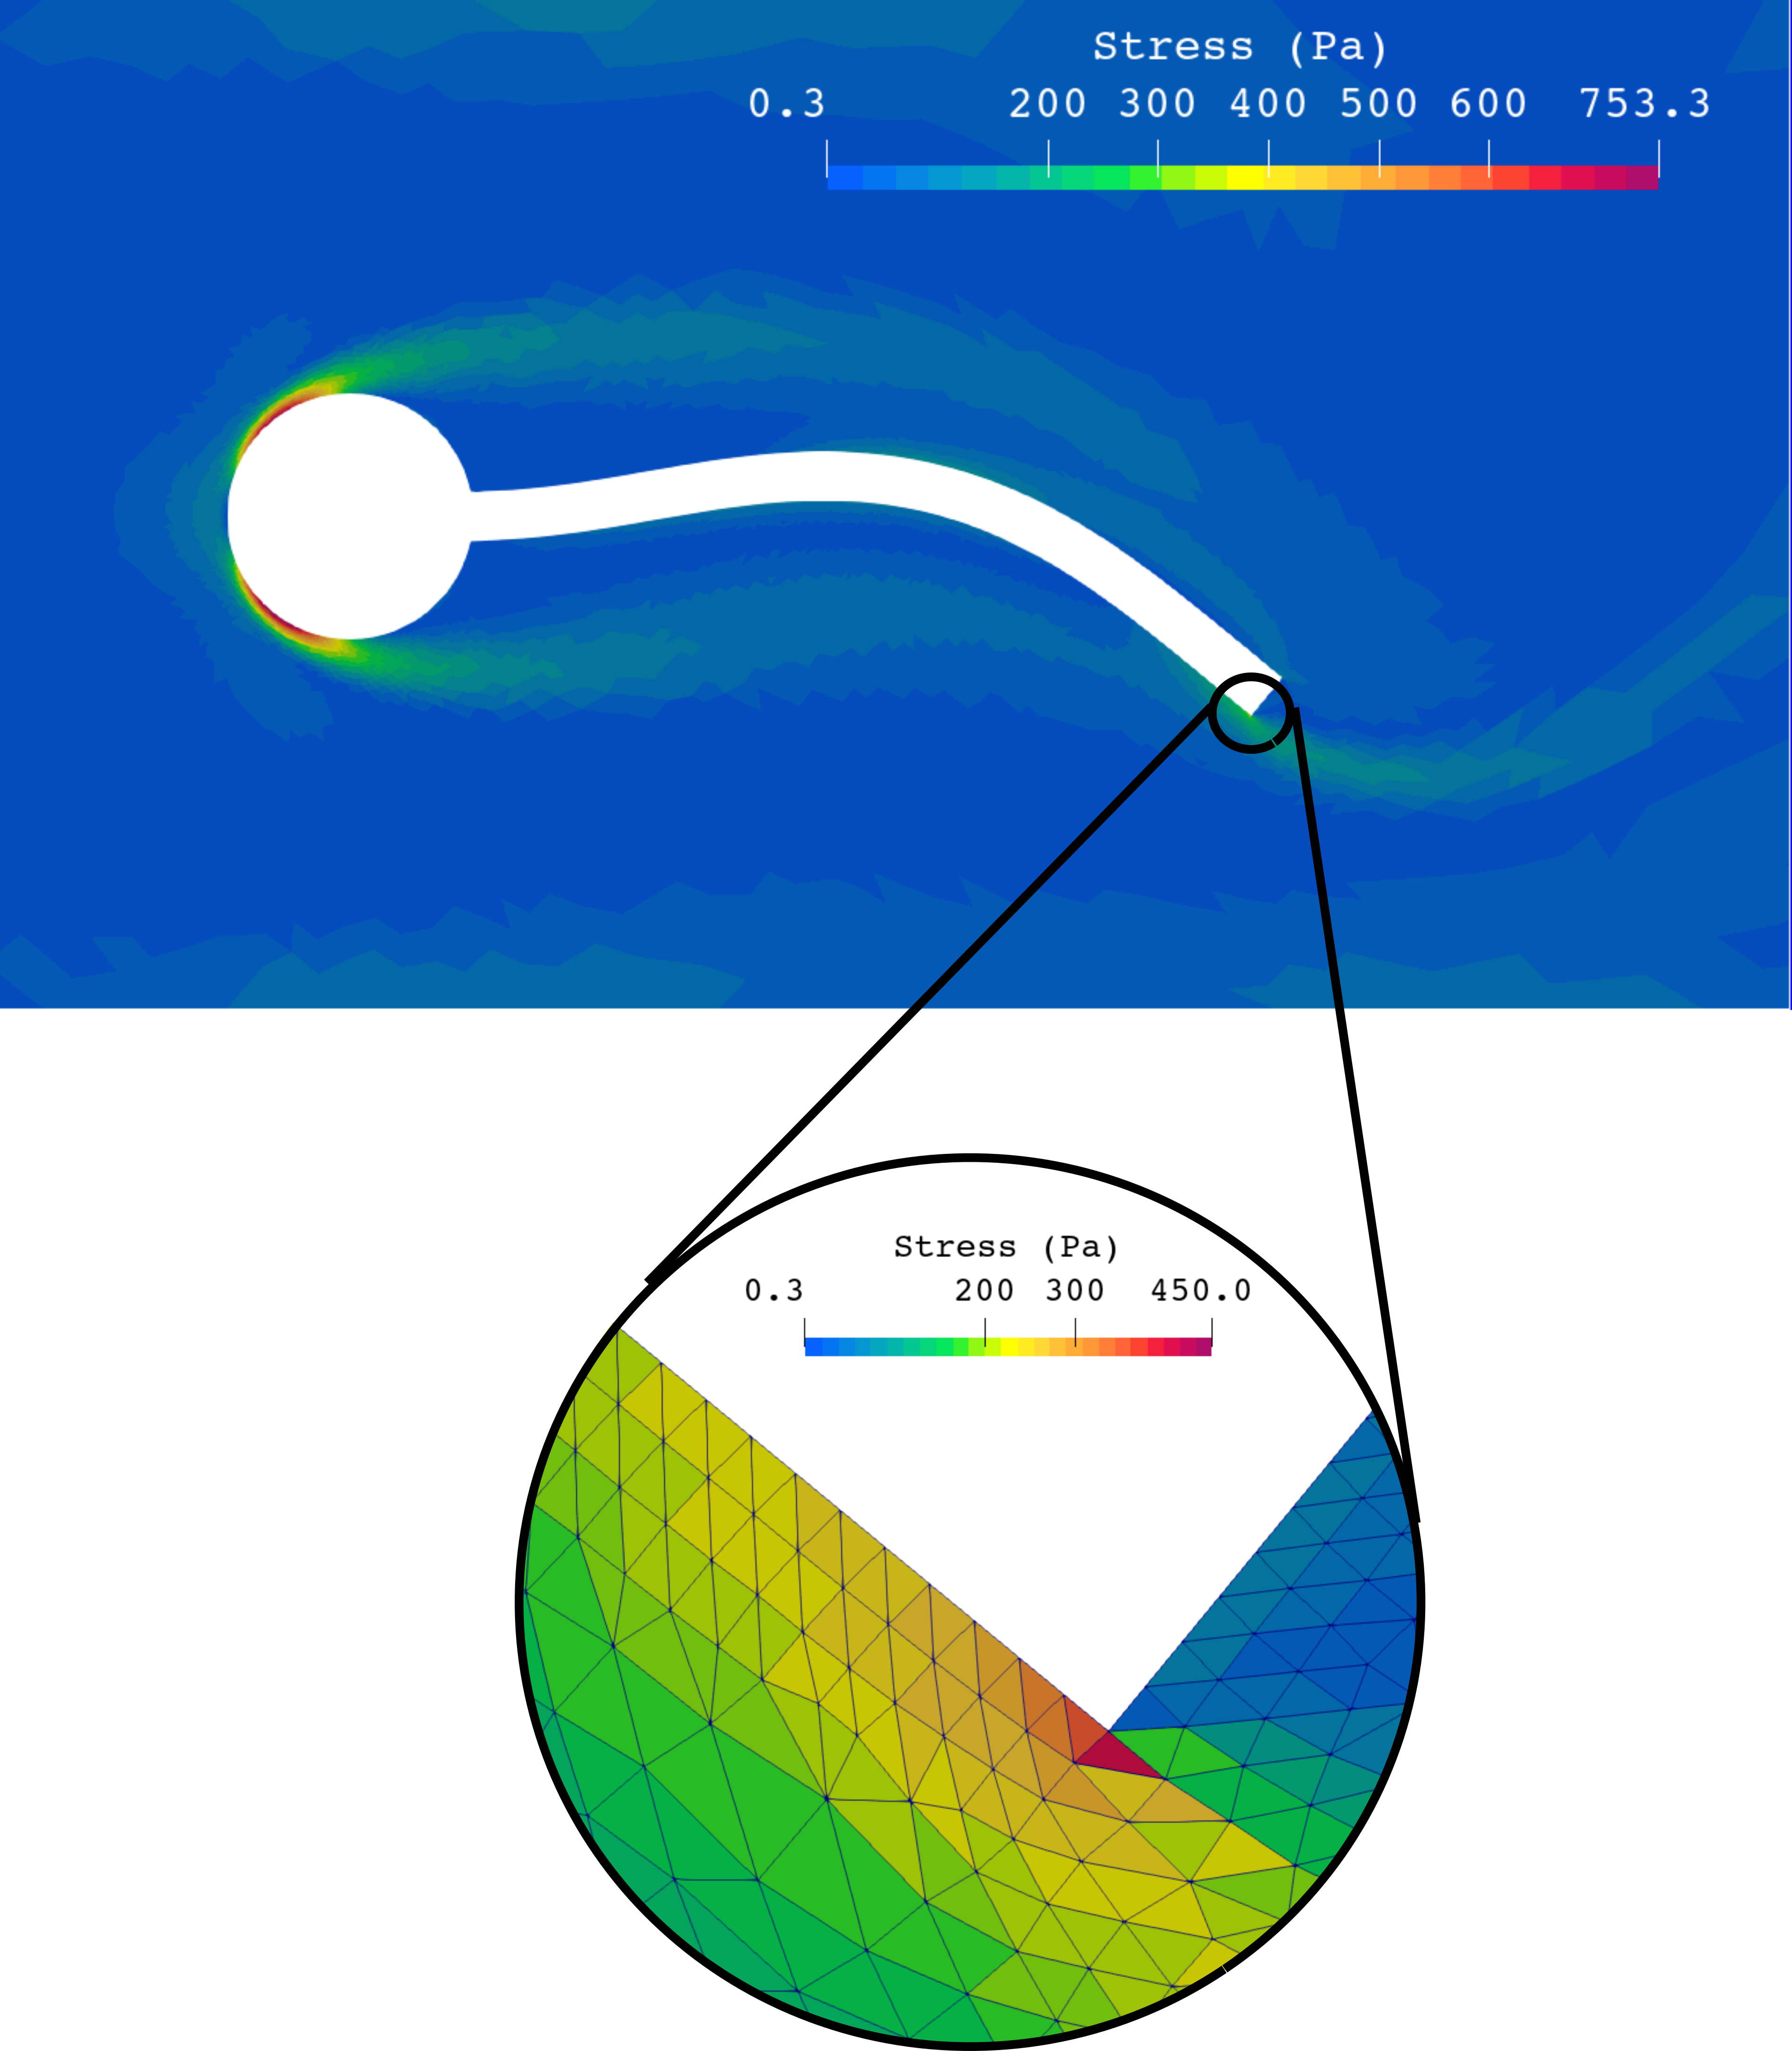
\includegraphics[scale=0.18]{Figures_Turek/UP_stress_zoom_circulo.png}}
    \vspace{1cm}
    \subfloat[three-field formulation]{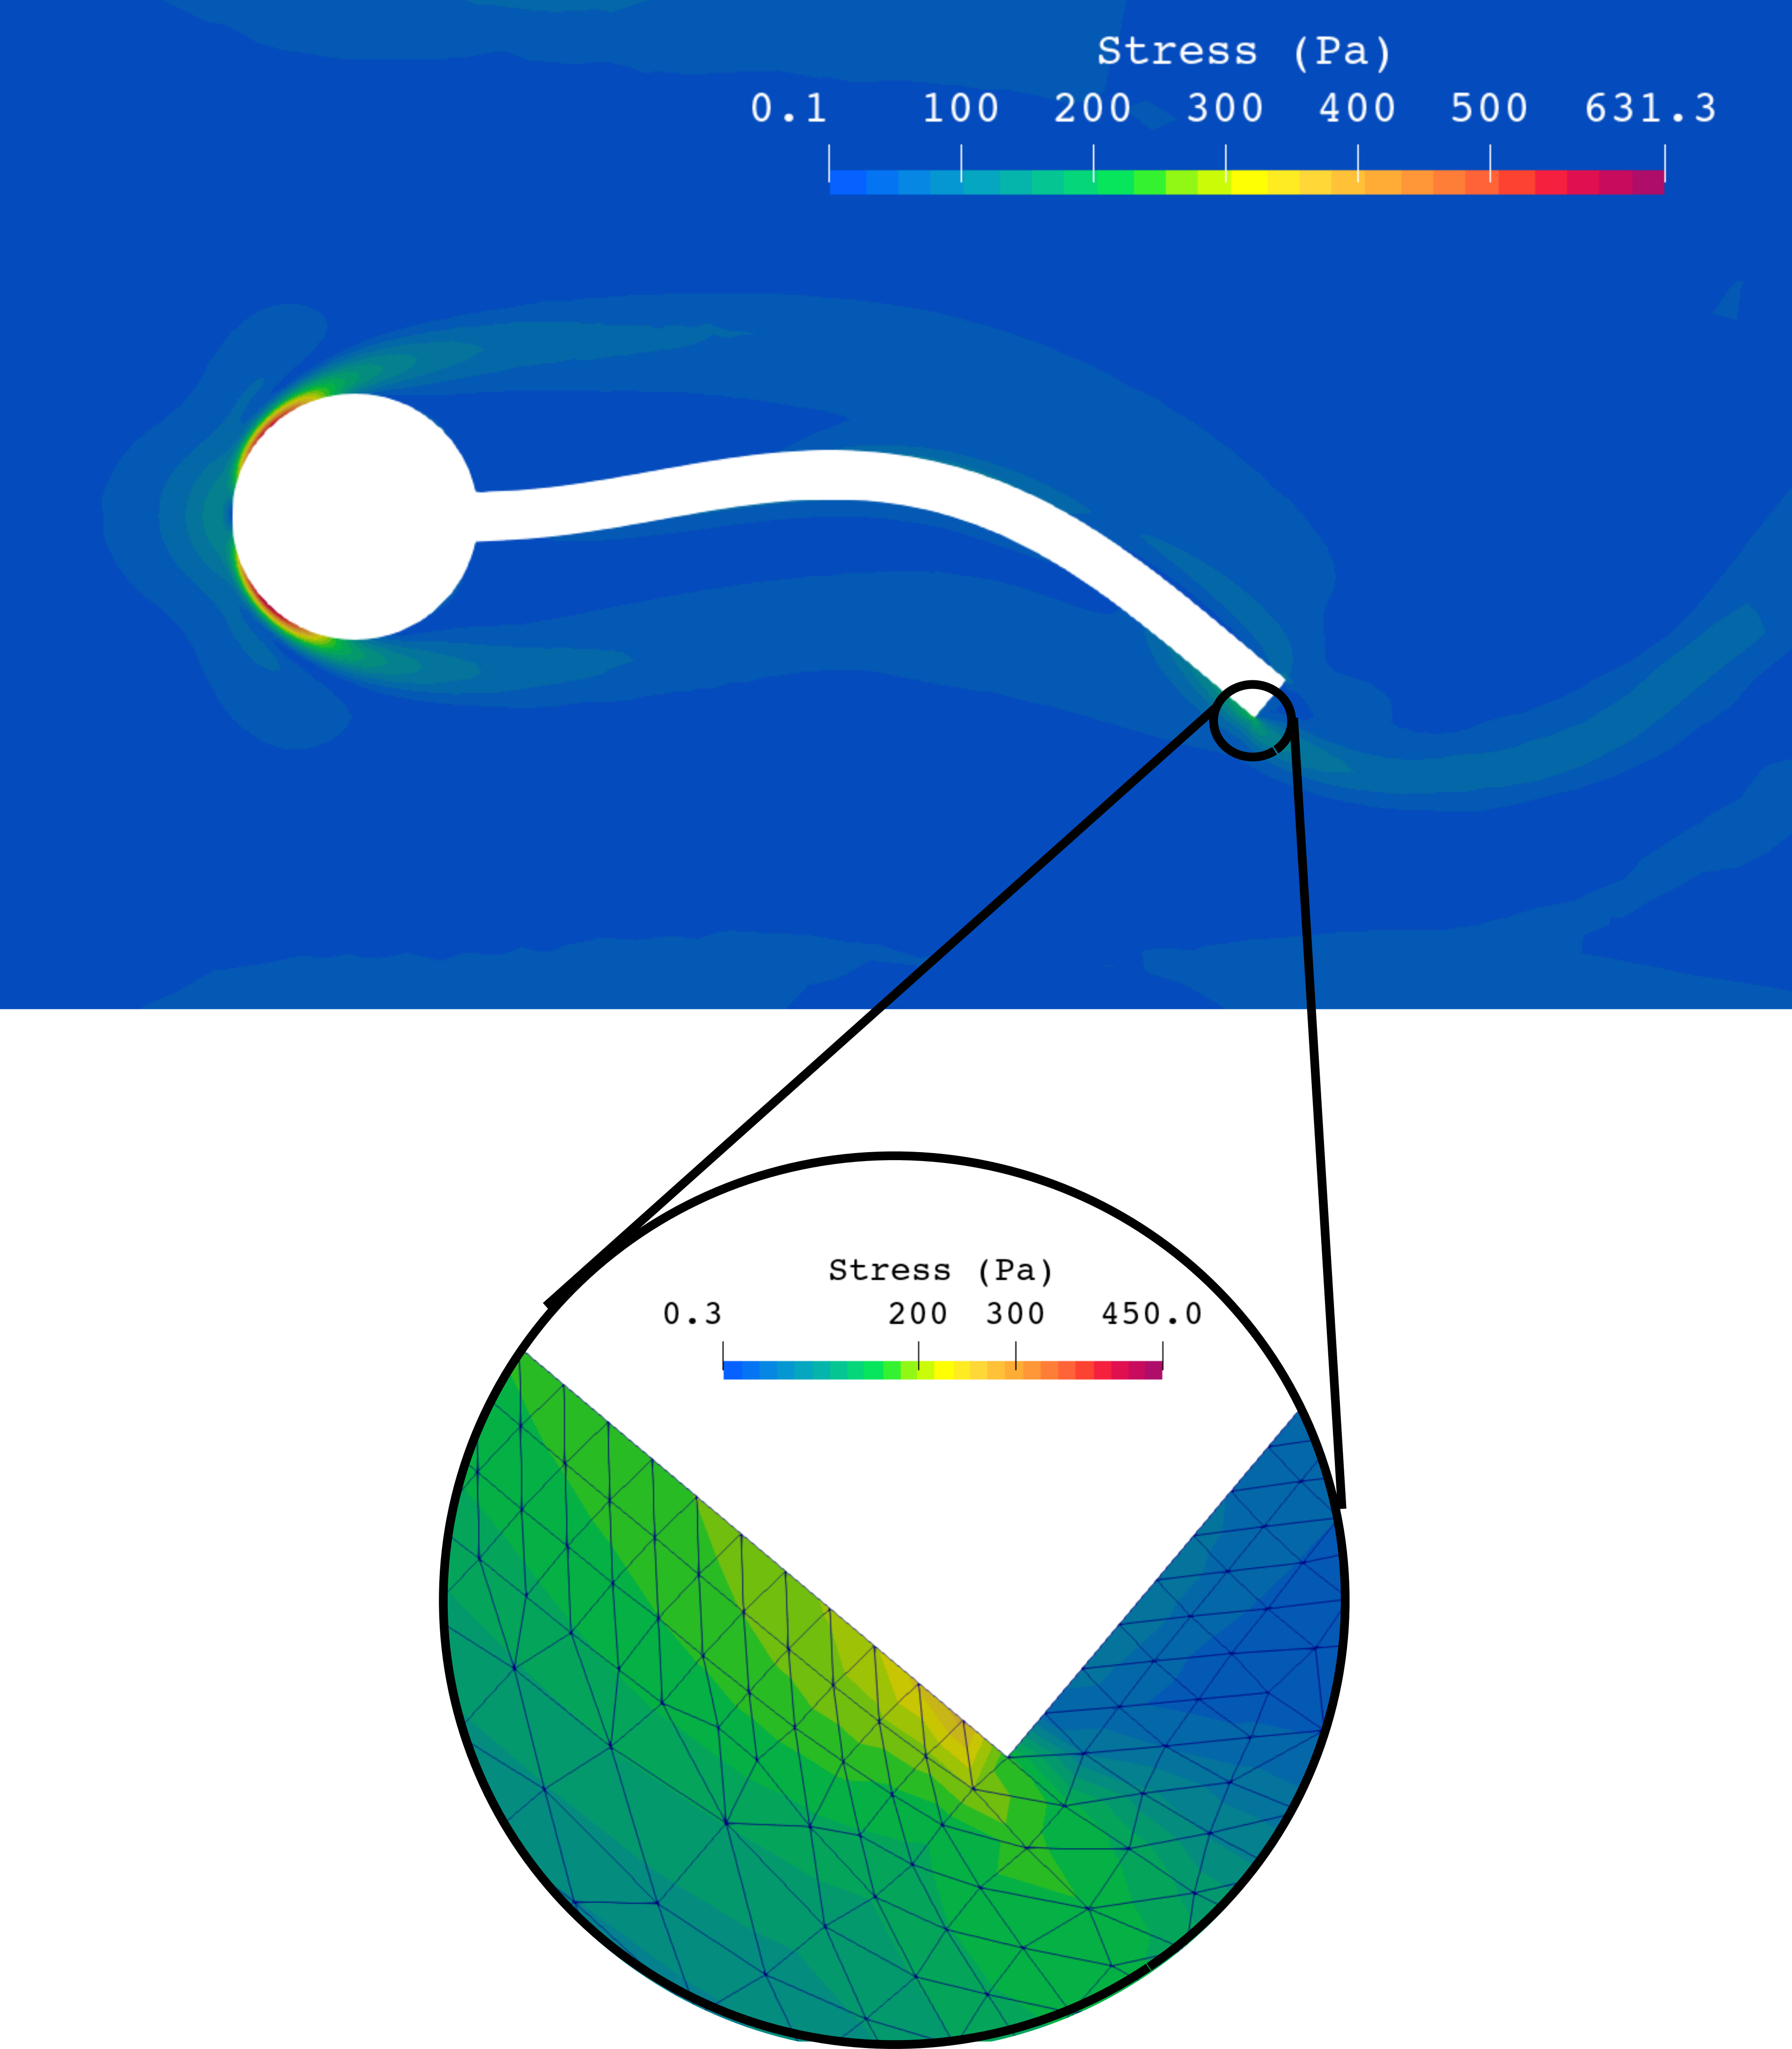
\includegraphics[scale=0.18]{Figures_Turek/UPS_stress_circulo.png}}
    \caption{Turek's test. Comparison of distribution of the stress field between the two-field formulation and the three-field one for the FSI2 test.}
    \label{fig:Turek-stresses}
\end{figure}

\subsubsection{FSI problem using a viscoelastic fluid flow}

In this subsection, the same problem is developed using a viscoelastic fluid and a Neo-Hookean model for the solid. First of all, numerical results are presented for the FSI1 case. Table \ref{tab:FSI1 Results} shows the displacement of the end of the beam structure at point A and the resulting forces exerted by the fluid on the whole submerged body. In this case the effect of viscoelasticity can be clearly analyzed. When the elasticity of the fluid increases, the vertical force exerted by the fluid (lift) also becomes higher. This phenomenon is in accordance with the study done in \cite{moreno2019logarithmic} in the classic flow over a cylinder case. One can conclude that higher vertical forces on the FSI boundary will cause the beam to show higher values of deformation.

\begin{table}[h!]
    \begin{centering}
        \begin{tabular}{ccccc}
            %\toprule 
            \hline
            \textbf{We}  & \textbf{x-disp of A [$10^{-4}$ m]} & \textbf{y-disp of A [$10^{-3}$ m]}  & \textbf{drag} [N] & \textbf{lift} [N] \tabularnewline
            %\toprule
            \hline
            0.0  & 0.2241 & 0.8202 & 14.263 & 0.7657  \tabularnewline
            0.2  & 0.2107 & 0.9384 & 14.703 & 0.7748   \tabularnewline
            0.4  & 0.1959 & 1.0650 & 15.250 & 0.7800 \tabularnewline
            0.6  & 0.1765 & 1.2020 & 16.089 & 0.7873   \tabularnewline
            0.8  & 0.1572 & 1.3100 & 17.038 & 0.7774   \tabularnewline
            1.0  & 0.1435 & 1.3440 & 18.003 & 0.7396  \tabularnewline
            1.2  & 0.1386 & 1.2520 & 19.054 & 0.6669   \tabularnewline
            %\bottomrule 
            \hline
        \end{tabular}
    \par\end{centering}
    \caption{Turek's test. Displacement at point A and forces exerted by the fluid on the beam for case FSI1.}
    \label{tab:FSI1 Results}
\end{table}

\begin{figure}[h!]
    \centering
    \subfloat[]{
    
\includegraphics[scale=0.925]{Figures_Turek/x-Displacement_A.eps}}
    \subfloat[]{
    
\includegraphics[scale=0.925]{Figures_Turek/y-Displacement_A.eps}}\\
    \subfloat[]{
    
\includegraphics[scale=0.925]{Figures_Turek/Lift.eps}}
    \subfloat[]{
    
\includegraphics[scale=0.925]{Figures_Turek/Drag.eps}}
    \caption{Turek's test. Results for FSI2.}
    \label{fig:FSI2 Results.}
\end{figure}

For the FSI2 problem, the evolution in time for displacements, lift and drag is computed for several We numbers. The maximum We regime that the algorithm is able to simulate using this mesh is ${\rm We} = 0.4$. Let us remark that the ``characteristic" We can vary depending on the problem configuration or the Reynolds number of the problem. In this case, the Reynolds number is higher than for the FSI1 problem, and therefore the maximum We  for which the algorithm is able to reproduce well-defined solutions is smaller than for case FSI1. In Fig. \ref{fig:FSI2 Results.} the tracking of the solution of point A along a second is performed to compare the different fluid flows. Note that the phases between plot cases have been conveniently adjusted in order to ease the comparisons. In the $y$-displacements, minimum and maximum peaks have slight variations. While for low Weissenberg numbers, higher than zero, a reduction of $y$-displacement is reported, when it grows up to ${\rm We}=0.3$ or ${\rm We}=0.4$ the displacements increase. This effect is connected with lift and drag force changes, which show a similar effect (see Fig.~\ref{fig:FSI2 Results.}). 

\subsection{Abdominal aortic aneurysms\label{subsec:aneurysm}}

As a final example, an abdominal aortic aneurysm is analyzed. The study of blood flow is important to understand the mechanisms behind the onset and progression of atherosclerosis \cite{Gharabi2016,Siasos2018}. Many studies related to abdominal aortic aneurysms consider the blood as a purely viscous fluid with constant viscosity, that is, a Newtonian fluid. In \cite{zaman2012blood,anand2013new} it is explained that blood can be modeled as an homogeneous shear-thinning and viscoelastic fluid characterized by the Oldroyd-B model. This is justified due to blood exhibiting non-Newtonian characteristics, mainly due to shear thinning viscosity and viscoelasticity related to stress relaxation and normal stress effects. Moreover, in the case of small arteries, the microstructure and rheological behavior of blood should not be neglected since the dimension of the blood particles is of the same order as that of the vessels. The parameters we used for modeling the blood flow are taken from \cite{elhanafy2019numerical}. 

In \cite{elhanafy2019numerical} a two-dimensional numerical study is performed in which the blood is modeled as a viscoelastic fluid, in which the Oldroyd-B constitutive model is used to represent the viscoelastic properties of the blood. Results show that at higher volumetric flow rates, which correspond to low shear rate situations, vortices are observed. The relative error with respect to the Newtonian flow model in these cases is of order 40 \% and cannot be neglected. Furthermore, in \cite{lopes2019} the influence of arterial mechanical properties on carotid blood flow is shown by comparing models with rigid and elastic walls. The conclusion that can be quickly drawn from the study is that the reciprocal influence of both fluid and solid (blood and artery) must be taken into account, so as not to overestimate the effect of rigid walls in the blood flow. In this example, we carry on a VFSI study to approximate the behavior of blood flow as a viscoelastic flow and to consider the artery as an hyperelastic Neo-Hookean material. 

\subsubsection{Setup}

The geometry of the problem  is displayed in Fig.~\ref{fig:aneurysm_geometry}. In this picture, one can observe the geometry of a channel with one single aneurysm. Particularly, in Fig.~\ref{fig:aneurysm_fluid_domain} the fluid arterial domain is plotted and in Fig.~\ref{fig:aneurysm_solid_domain} the solid domain, where a membrane thickness of $d=0.001$~m is considered, following the one described for the carotid case in \cite{lopes2019}. Finally, the fully coupled model is drawn in Fig.~\ref{fig:aneurysm_full_domain}, where a transversal cut is done to indicate the lengths adopted for the 3D domain generation. In our case, $D=0.008$ m is the diameter of the artery at the inlet and outlet sections, $R=D/2$ is the aneurysm ratio, $L_T=7.5D$ is the domain total length, and the other dimensions are set as $L_1=2.5D$ and $L_2=5D$. Also $D_1=2D$ is the maximum diameter adopted in the domain for the artery. Moreover, the geometry has been constructed using the curve
\begin{equation}
    y=\left(\dfrac{D_1-D}{2}\right)\left[1+\sin\left(\dfrac{2\pi(x-L_1)}{L_2}-\dfrac{\pi}{2}\right)\right]+\dfrac{D}{2} \qquad L_1\leq x \leq L_2,
    \label{eq:aneurysm_curve_equation}
\end{equation}
which has been revolutionized over the longitudinal axis ($x$).

\begin{figure}[h!]
    \centering
    \subfloat[Fluid domain]{
    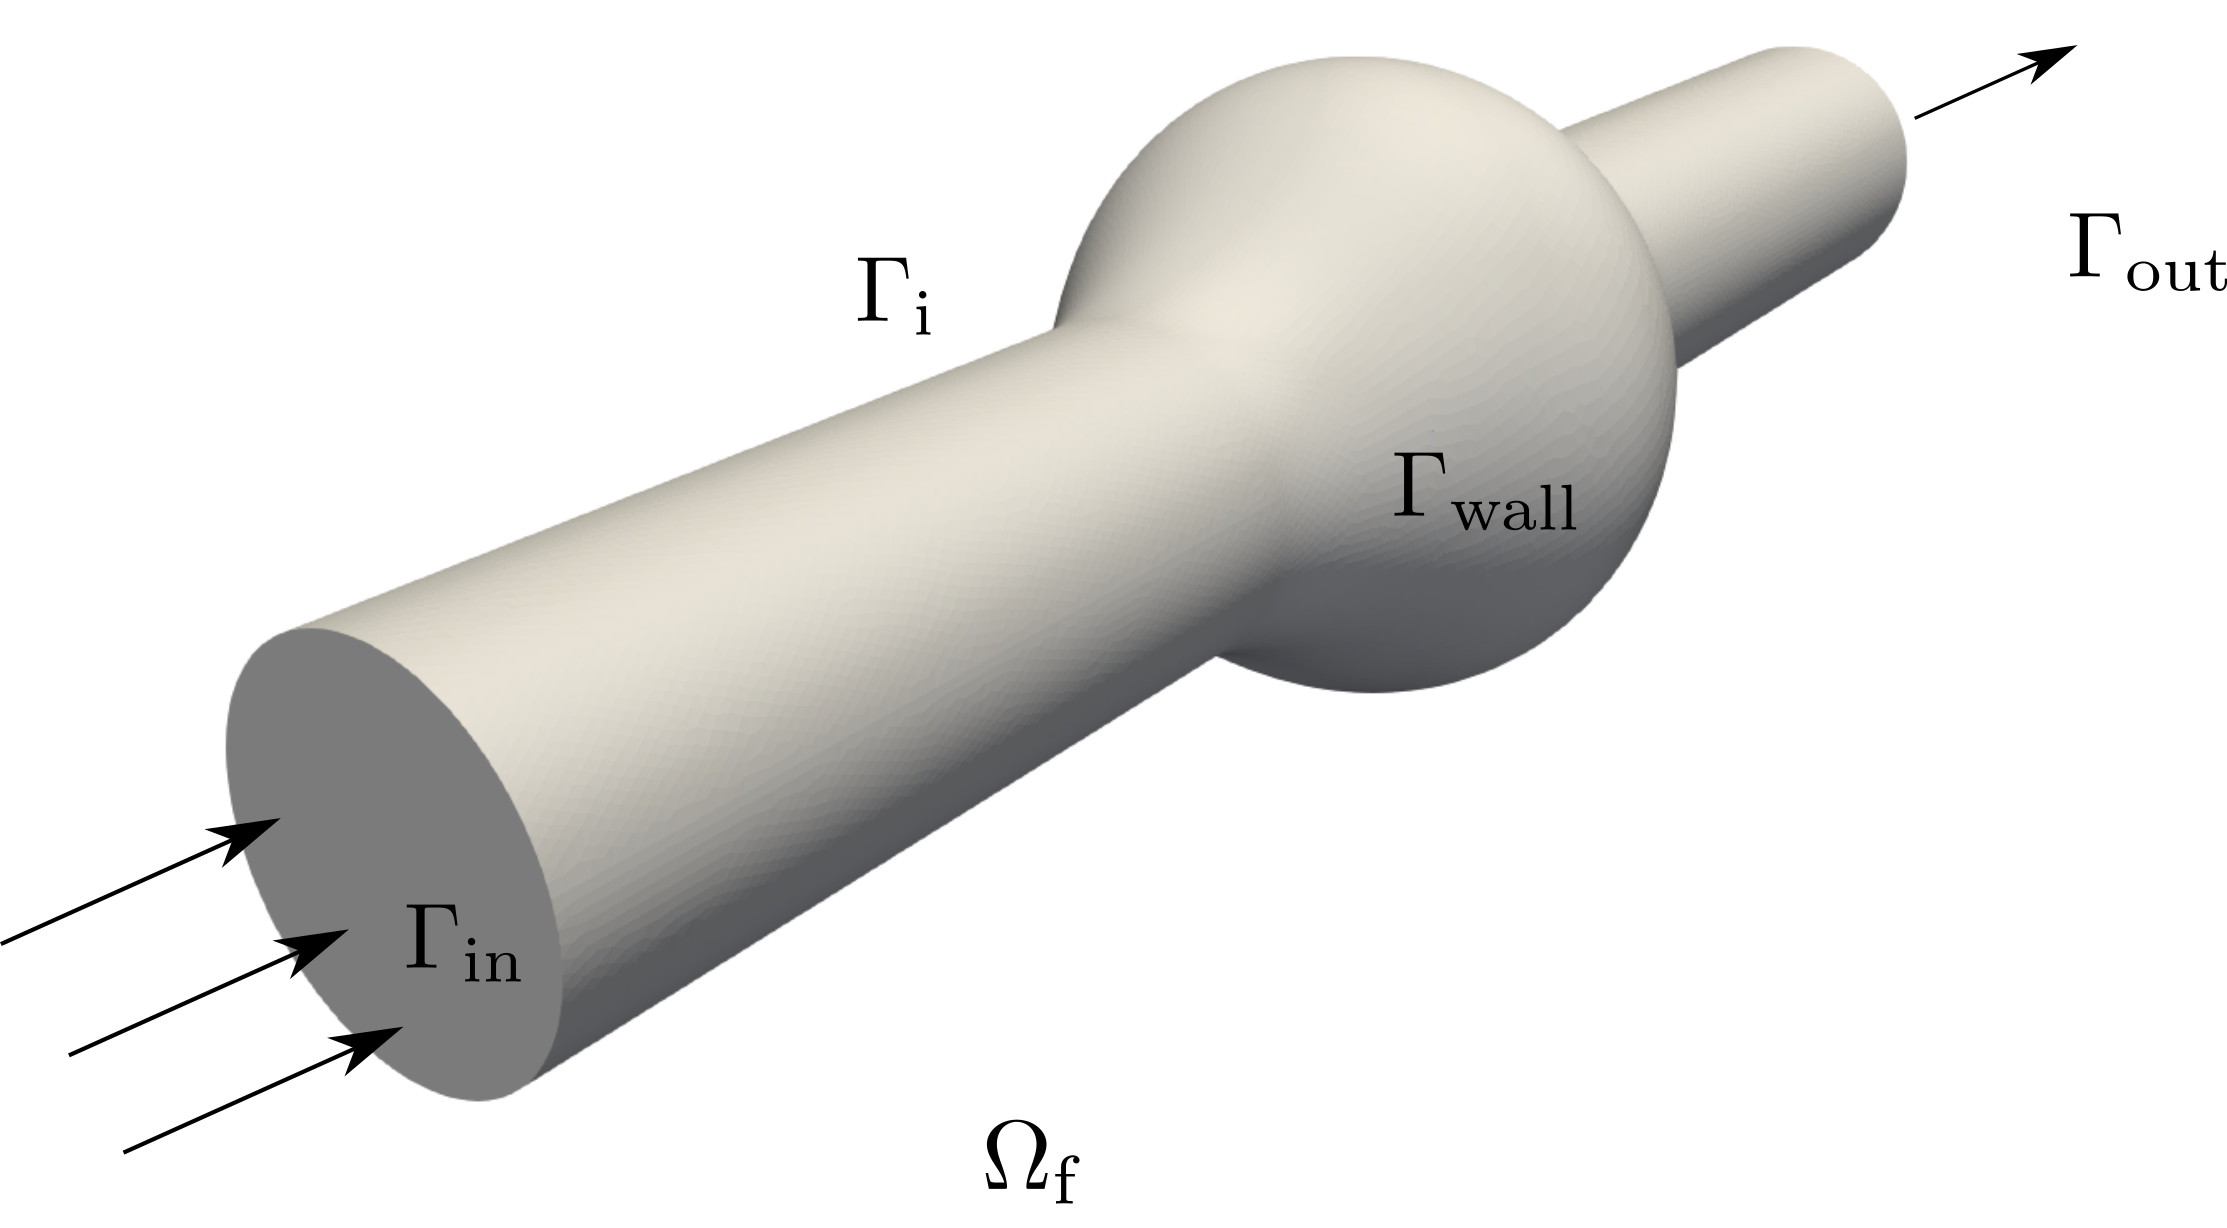
\includegraphics[scale=0.28]{Figures_aneurism/fluid_domain.png} \label{fig:aneurysm_fluid_domain}}
    \subfloat[Solid domain]{
    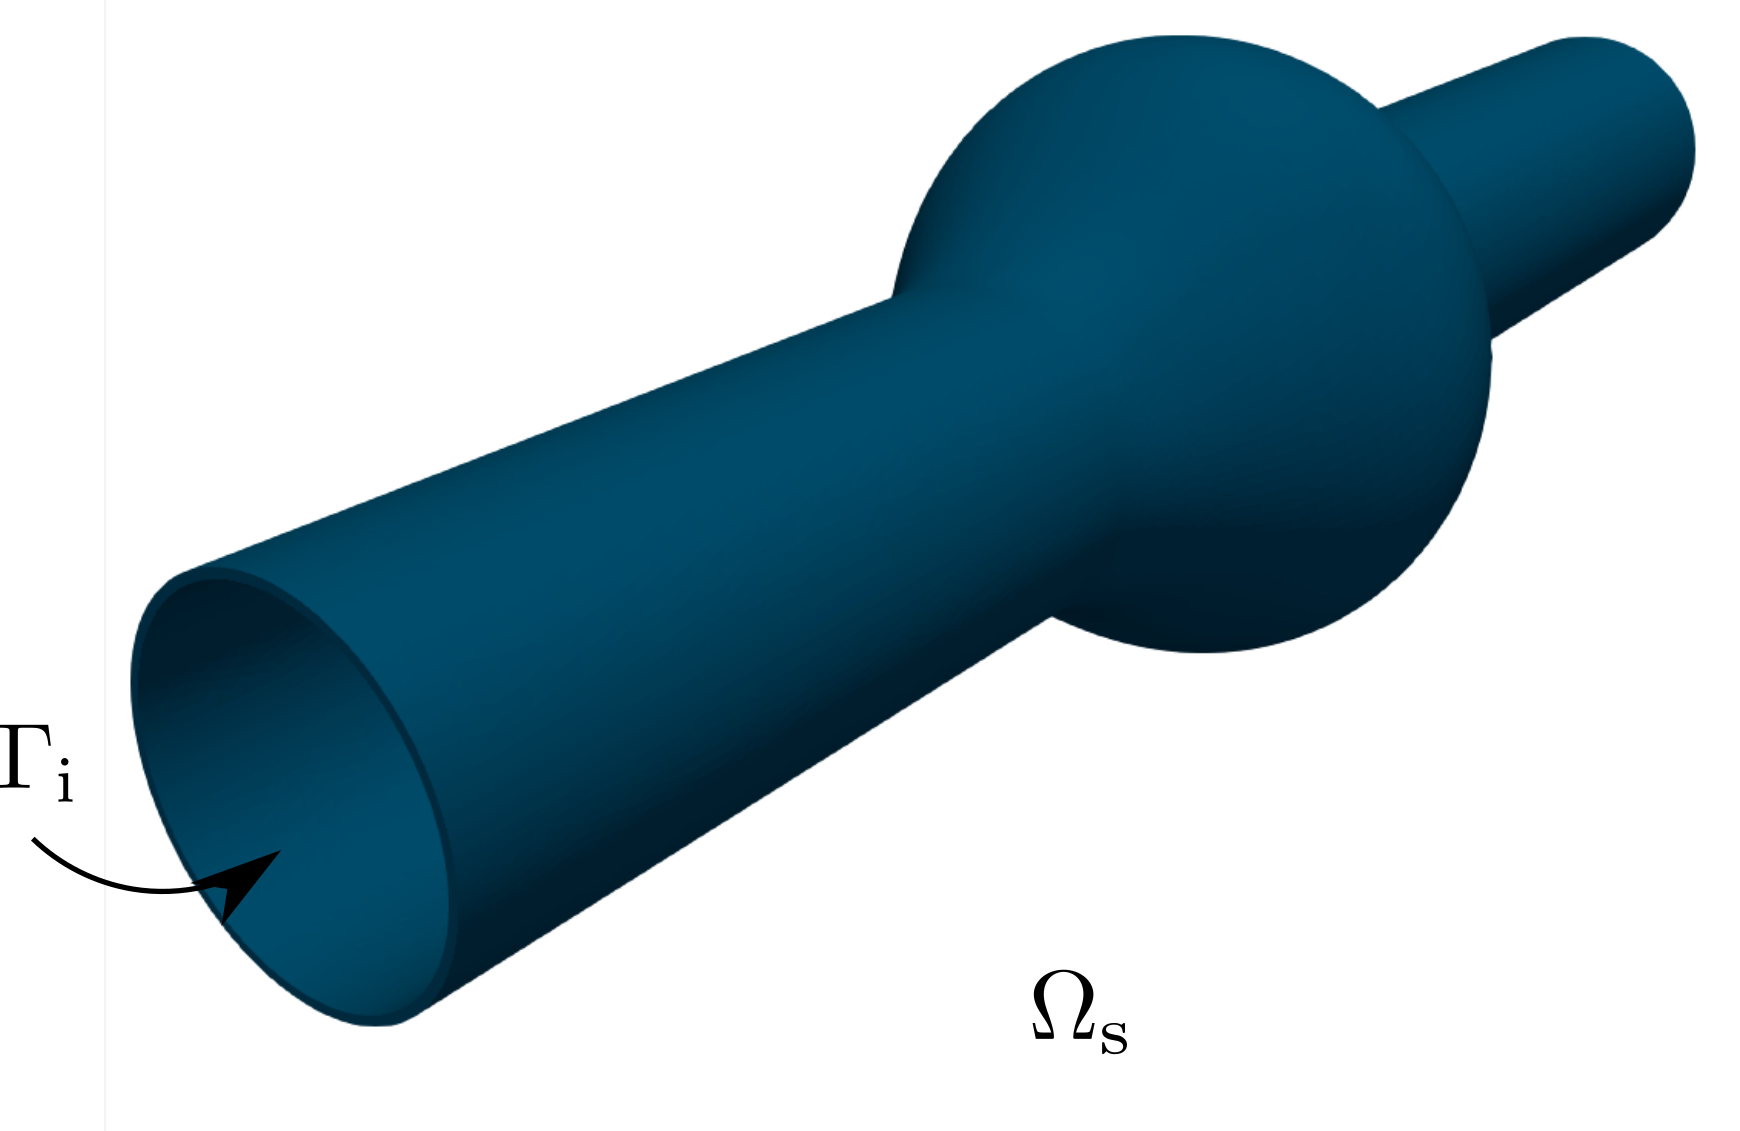
\includegraphics[scale=0.28]{Figures_aneurism/solid_domain.png} \label{fig:aneurysm_solid_domain}}\\
    \subfloat[Full domain]{
    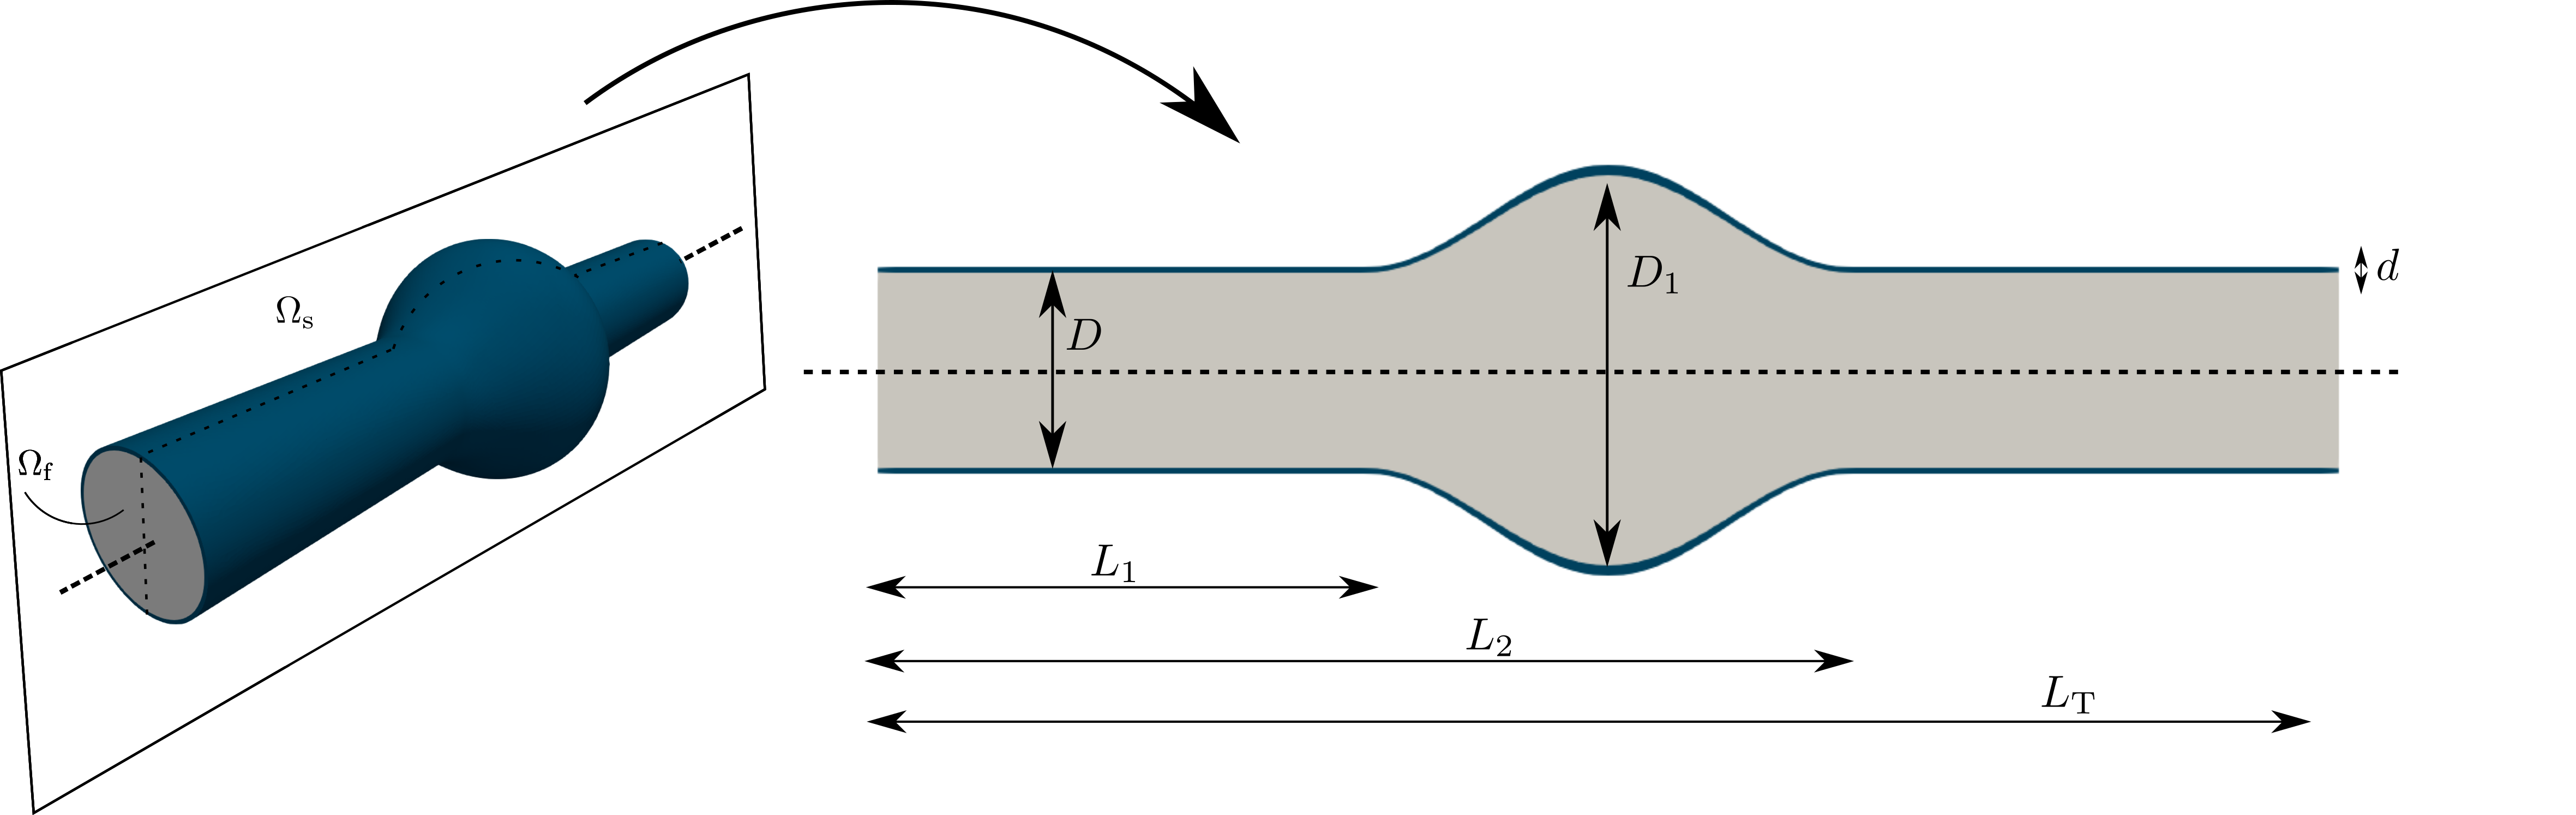
\includegraphics[scale=0.3]{Figures_aneurism/full_domain.png} \label{fig:aneurysm_full_domain}}
    \caption{Aneurysm problem. Geometry.}
    \label{fig:aneurysm_geometry}
\end{figure}

Once the geometry has been defined, the fluid and solid properties will be described.  First of all, the blood in the artery is considered as a Newtonian fluid, and later as a viscoelastic one.  For the Newtonian cases performed, the blood density is $\rho_{\rm{f}} = 1\,060\text{ kg}/\text{m}^3$ and the dynamic viscosity $\mu_{\rm{f}} = 3.5 \cdot 10^{-3}\text{ Pa}\cdot\text{s}$; for the viscoelastic fluid model, the properties are $\viscs = 3.19 \cdot 10^{-3}\text{ Pa}\cdot\text{s}$ for the solvent viscosity and  $\viscp = 4 \cdot 10^{-4}\text{ Pa}\cdot \text{s}$ for the polymeric viscosity.  In other words, the total viscosity is set to $\mu_{\rm{f}}^0 = 3.49\text{ Pa}\cdot \text{s}$ and $\beta=0.88$. Concerning the relaxation time, it is set to $\lambda=0.06$~s.  Secondly, for the solid domain, which models the vessel wall deformation, an hyperelastic Neo-Hookean law is considered.  Regarding the mechanical properties, the density is $\rho_{\rm{s,0}} = 1\,120\text{ kg}/\text{m}^3$, the Poisson ratio is $\nu_{\rm{s}}= 0.45$ and elastic modulus is $E_{\rm{s}}=1.106\cdot 10^{6}~\text{Pa}$.

For the fluid domain, a no-slip boundary condition is imposed over the walls and a fully developed flow is assumed at the artery inlet, following the expression
\begin{center}
\begin{tabular}{ccc}
$u_x(0,y,z,t)=u_{\max} \left(1-\dfrac{(z^2+y^2)}{R^2}\right),$  & $u_{y}(0,y,z,t)=0,$ & $u_{z}(0,y,z,t)=0$.
\end{tabular}
\par\end{center}
Note that $u_x$ is the main direction of the flow in the artery; the average velocity at the inlet is $\bar{u}=0.05968~\rm{m}/\rm{s}$ taking $u_{\max}= 0.11936 ~\rm{m}/\rm{s}$ as the maximum velocity reached at the inlet. The flow rate is $Q=3\cdot10^{-6} \text{ m}^3/\rm{s}$. This is the maximum flow rate adopted by the reference paper \cite{elhanafy2019numerical}. While in the Newtonian regime stresses are considered free in the inlet, for the viscoelastic fluid flow case those have been fixed associated to the parabolic velocity profile. The artery exit is considered stress free, but to avoid fluid recirculations in the exit only the first component of the velocity is set to be free. Lastly, note that the Reynolds number associated to this regime is 139.7 and, for the viscoelastic fluid flow, the We number is 0.447.

Relative to the solid model, the boundaries adjacent to the inlet and outlet are fixed. On the remaining boundaries of the solid, a stress free condition is considered, which basically allows the solid to deform in any direction.

Concerning the generated mesh, it is unstructured and the domain is discretized using  582\,804 tetrahedral FEs for the fluid domain, while the solid one has 286\,597 hexahedral elements. The minimum element size, found on the walls of the fluid domain and in the solid domain, is about $h_{\min}=0.00025$. The time step size is set to $\delta t=0.0025$. SI units are used throughout.

\subsubsection{Results}

As mentioned earlier, a similar study is performed in \cite{elhanafy2019numerical} for a 2D case to highlight the importance of choosing a viscoelastic fluid for modeling the human blood; however, we also incorporate the interaction with a solid membrane, as suggested in \cite{lopes2019}. Its effect is quantified in the following.

Fig. \ref{fig:aneurysm_streamlines} shows the fluid flow streamlines. Specifically, Fig. \ref{fig:aneurysm_stream_viscoelastic3D} plots the streamlines in the full 3D model. Here, the vortices of the flow, which are located close to the aneurysm walls, can be clearly observed. For a better comprehension of these vortices, both Fig.~\ref{fig:aneurysm_stream_newtonian} (Newtonian case) and Fig.~\ref{fig:aneurysm_stream_viscoelastic} (viscoelastic case) are displayed in a transversal cut in the $z=0$ plane. Note that this plane is in the middle of the domain. In contrast with the Newtonian fluid, it is remarkable how the center of vortices is moved on downstream for the viscoelastic case. Note that for this Reynolds number the solution has axial symmetry. 

\begin{figure}[h!]
    \centering
    % \subfloat[Newtonian fluid]{
    % 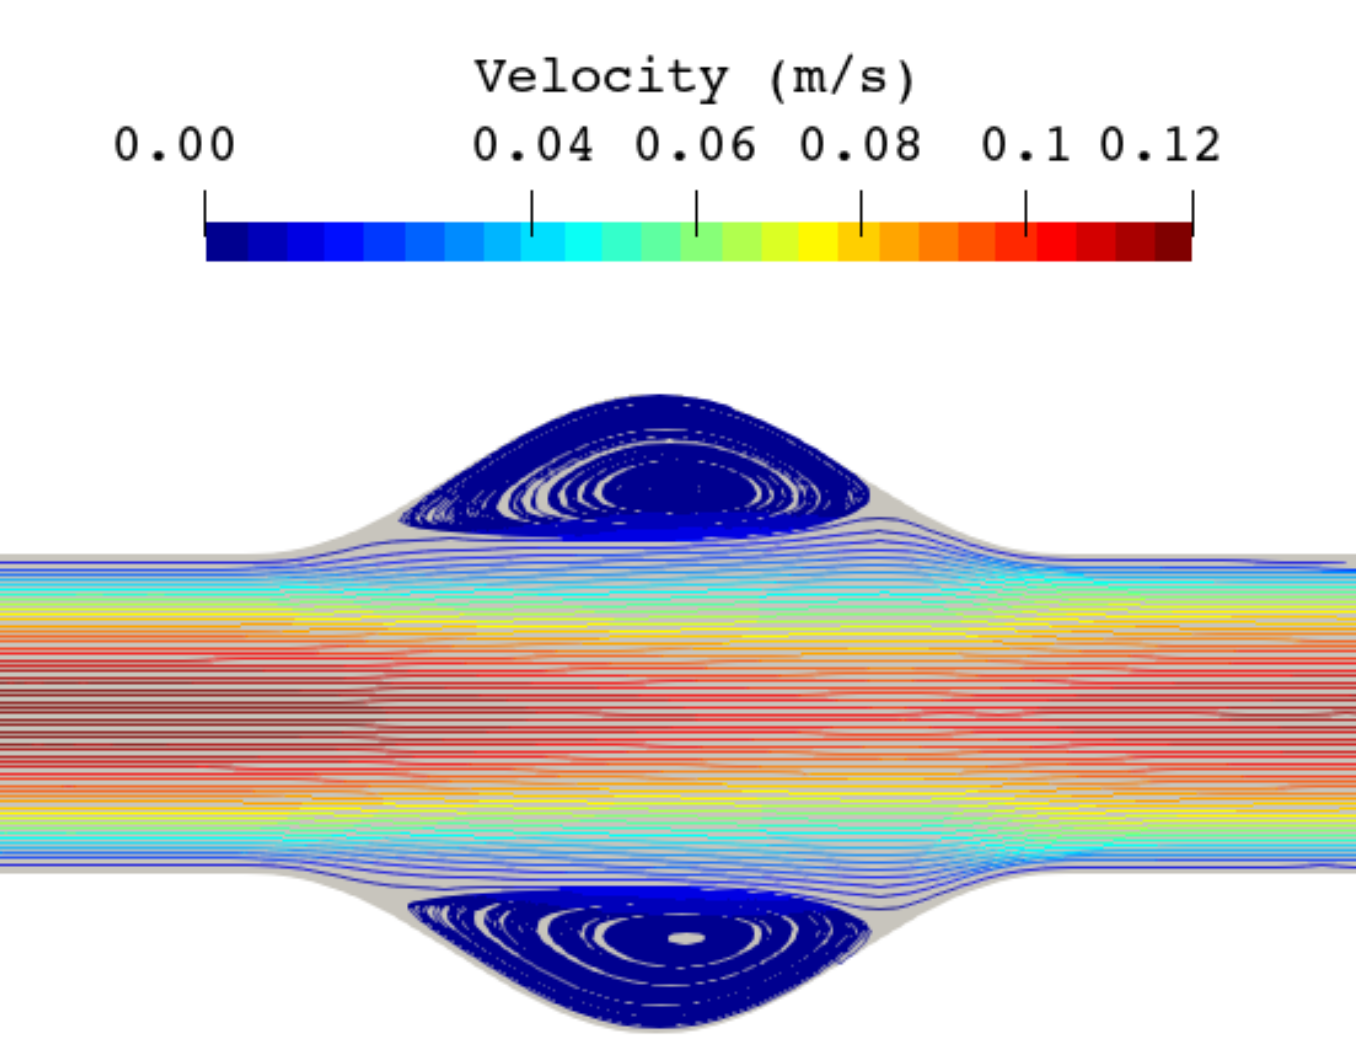
\includegraphics[scale=0.3]{Figures_aneurism/streamlines_newtonian.png} \label{fig:aneurysm_stream_newt}}\\
    \subfloat[Fluid domain]{
    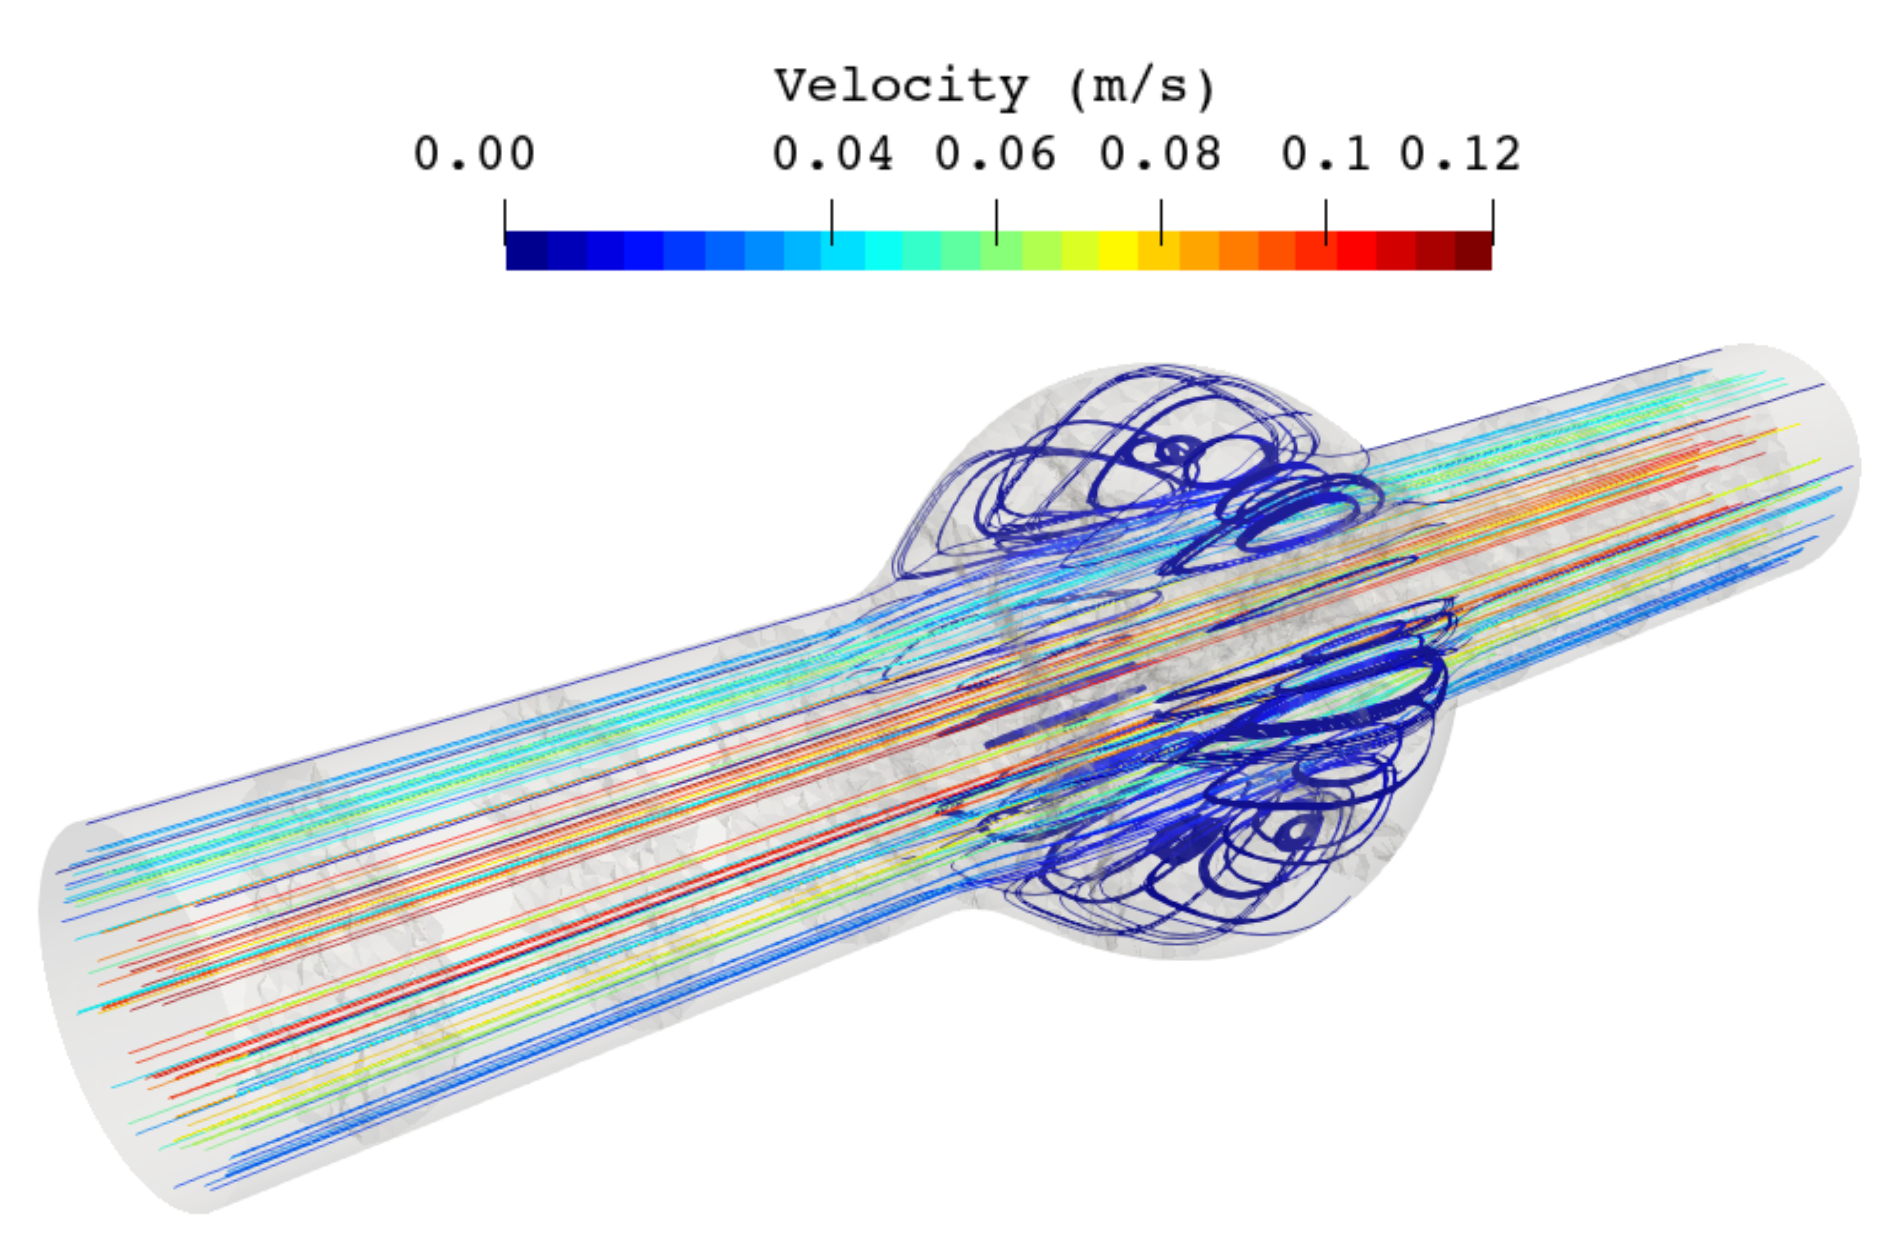
\includegraphics[scale=0.5]{Figures_aneurism/Streamlines3D.png} \label{fig:aneurysm_stream_viscoelastic3D}}\\
    \subfloat[Streamlines of the Newtonian fluid in a cut in the $z=0$ plane.]{
    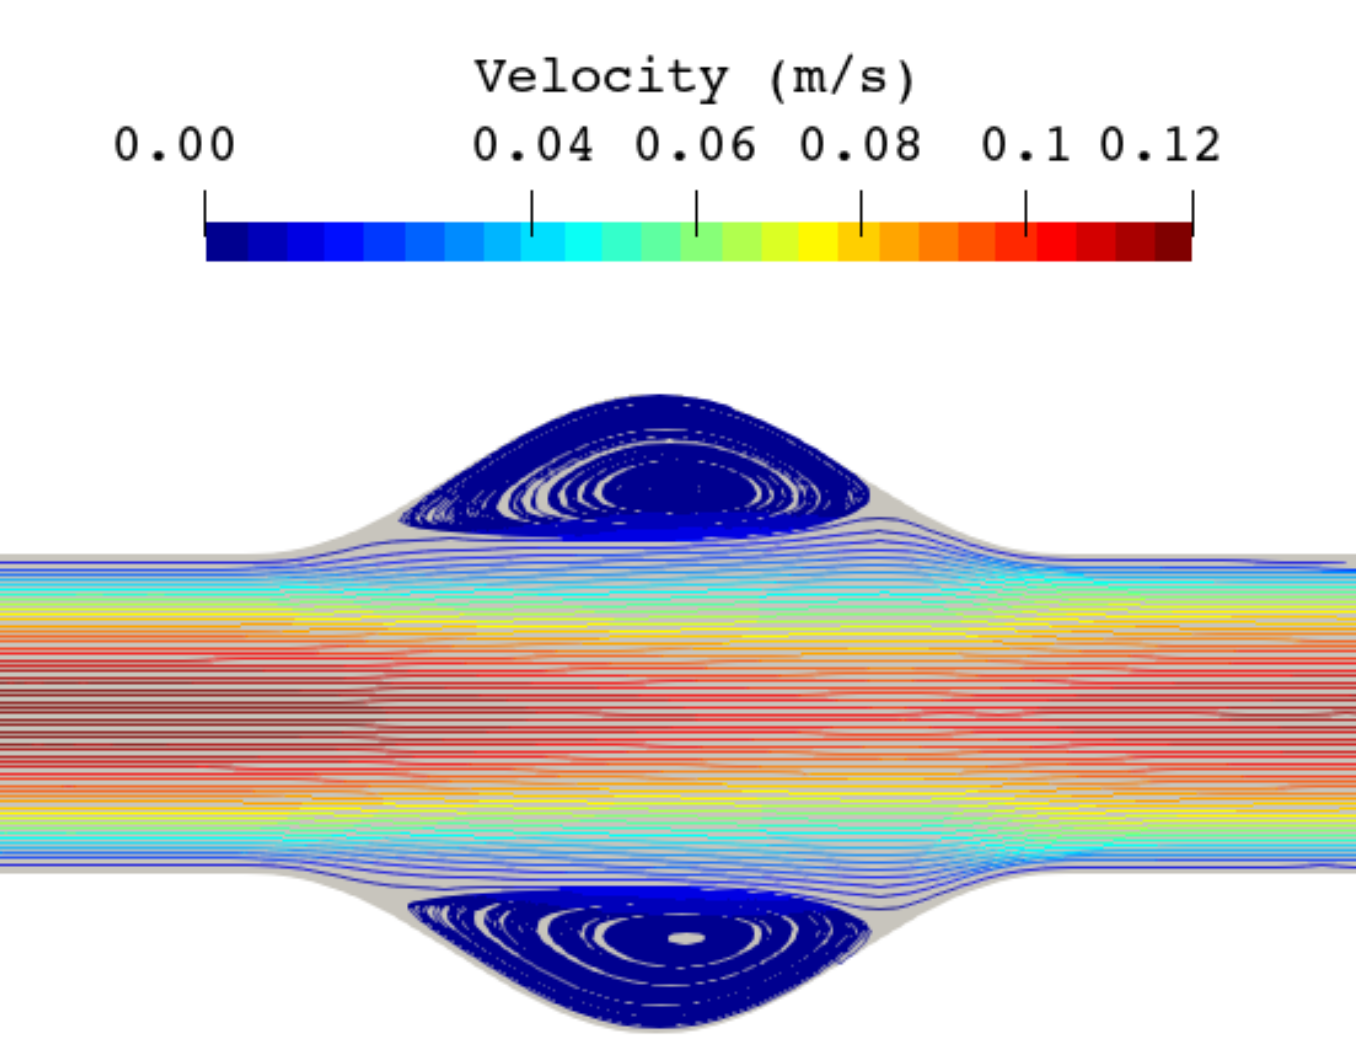
\includegraphics[scale=0.5]{Figures_aneurism/streamlines_newtonian.png} \label{fig:aneurysm_stream_newtonian}}\hskip0.4cm
    \subfloat[Streamlines of the viscoelastic fluid in a cut in the $z=0$ plane.]{
    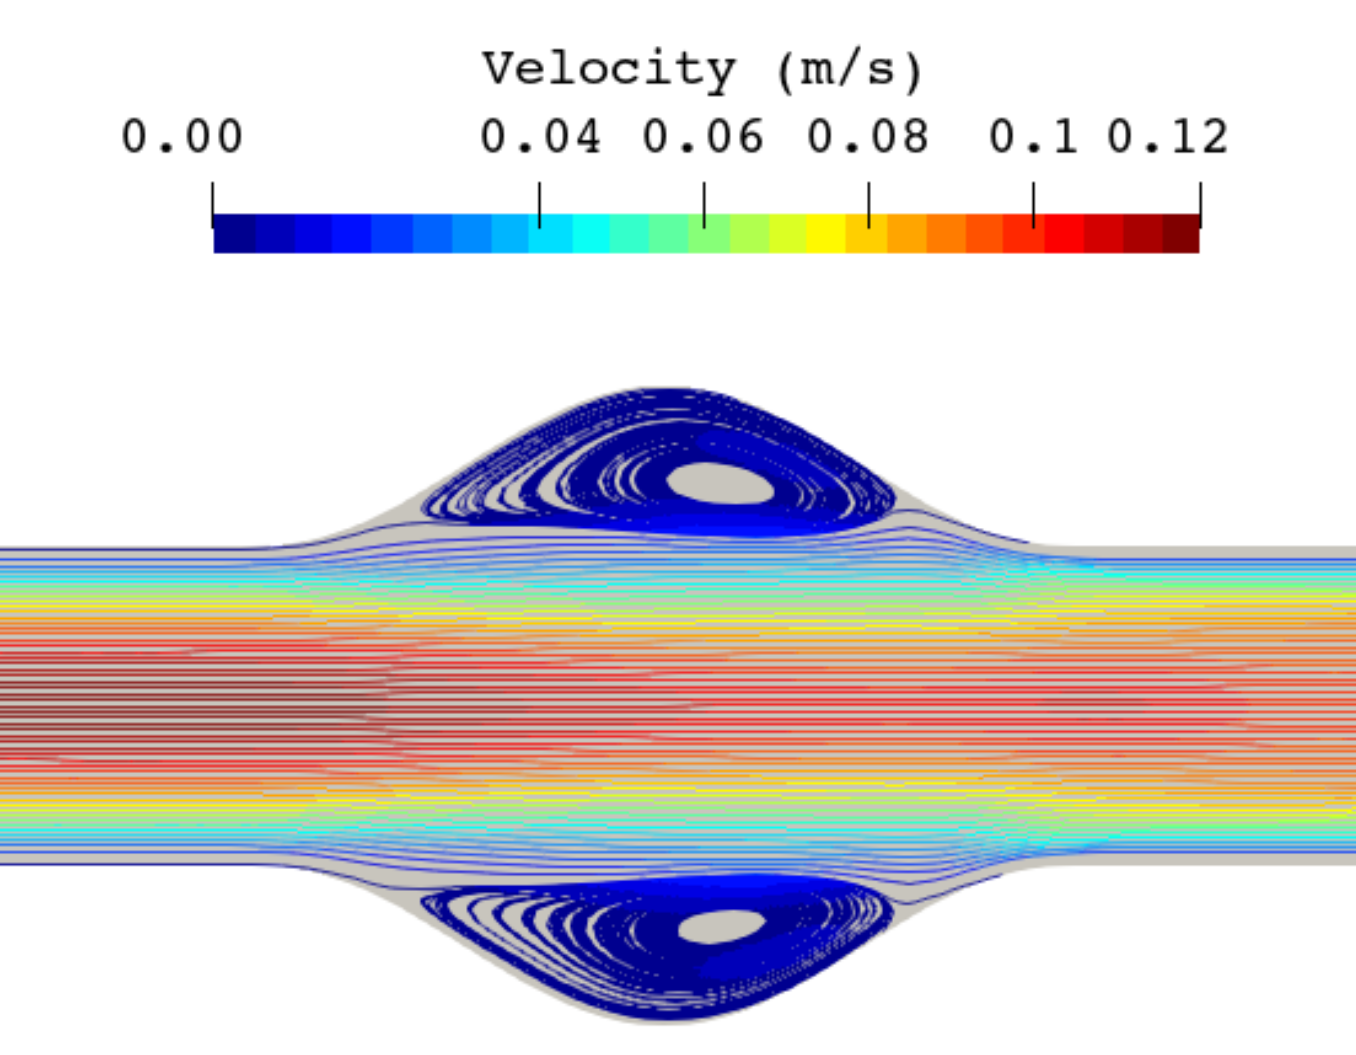
\includegraphics[scale=0.5]{Figures_aneurism/streamlines_viscoelastic.png} \label{fig:aneurysm_stream_viscoelastic}}
    \caption{Streamlines in the full domain and in a transversal cut, coloured with the norm of the velocity.}
    \label{fig:aneurysm_streamlines}
\end{figure}

In Fig. \ref{fig:aneurysm_comparison_viscoelastic} the distribution of the dominant component of the stresses is shown on the plane $z=0$. The Newtonian case shows smaller values than the viscoelastic case and the maximum peaks are reached at the center of the channel. However, the viscoelastic case accumulates stresses on the walls immediately downstream of the aneurysm. This is graphically evaluated in Fig.~\ref{fig:aneurysm_norm}, where the norm of stresses over the top line in the $z=0$ plane is plotted. The difference of magnitude in this location is notable, as reported in \cite{elhanafy2019numerical}. The vertical lines indicate the region of the aneurysm. This effect is important when dealing with aneurysms, and should not be neglected. Finer elements around the walls would be needed to obtain smoother solutions.  

\begin{figure}[h!]
    \centering
    \subfloat[Newtonian fluid]{
    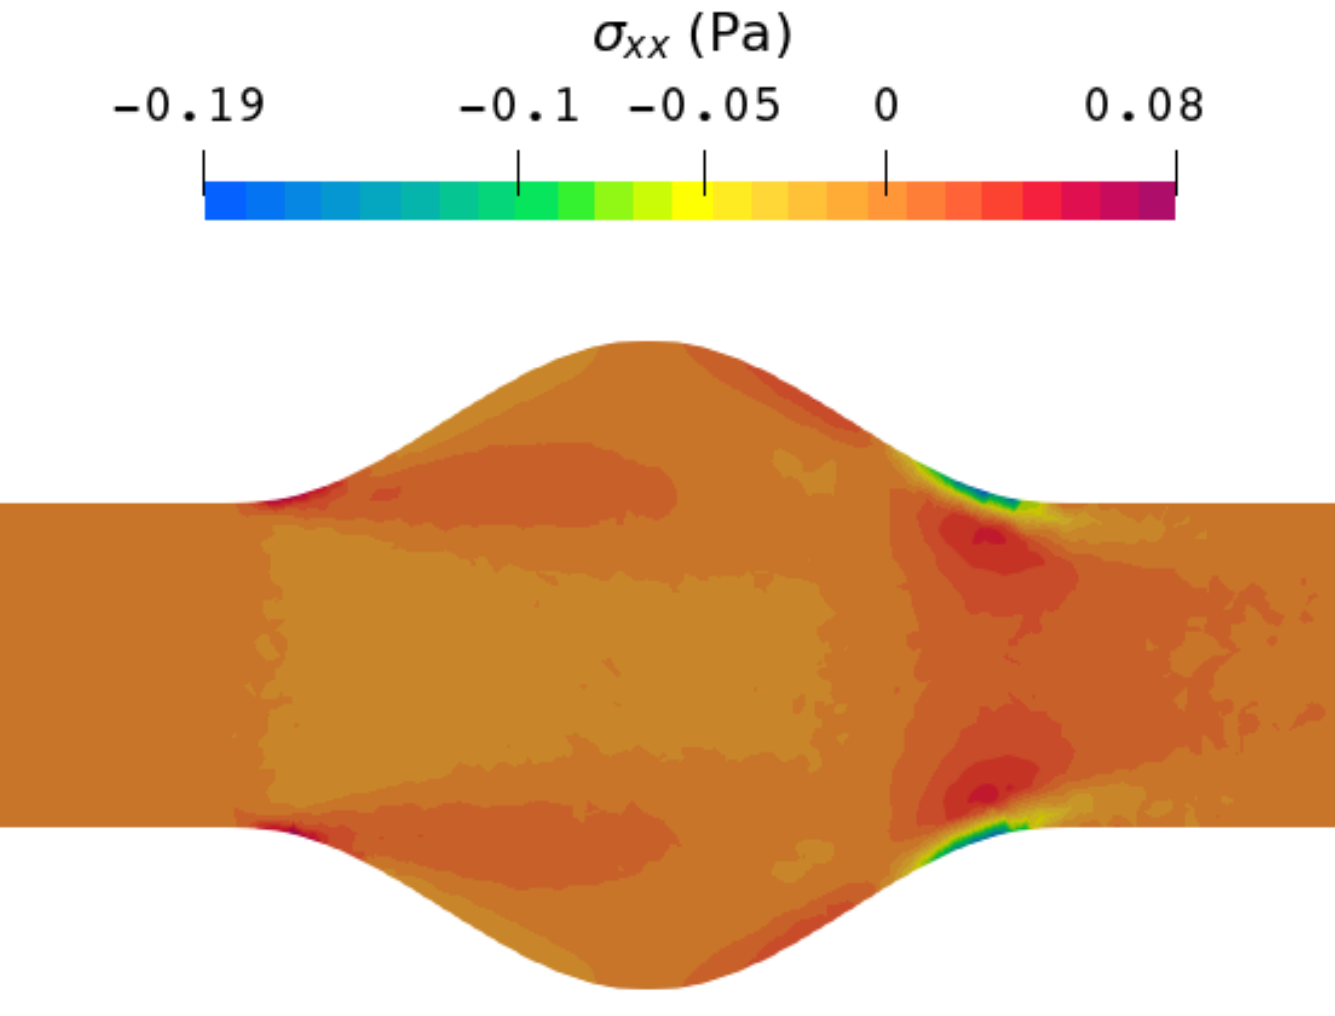
\includegraphics[scale=0.5]{Figures_aneurism/stressXX_nextonian.png} \label{fig:aneurysm_stress_newt}} 
    \subfloat[Viscoelastic fluid]{
    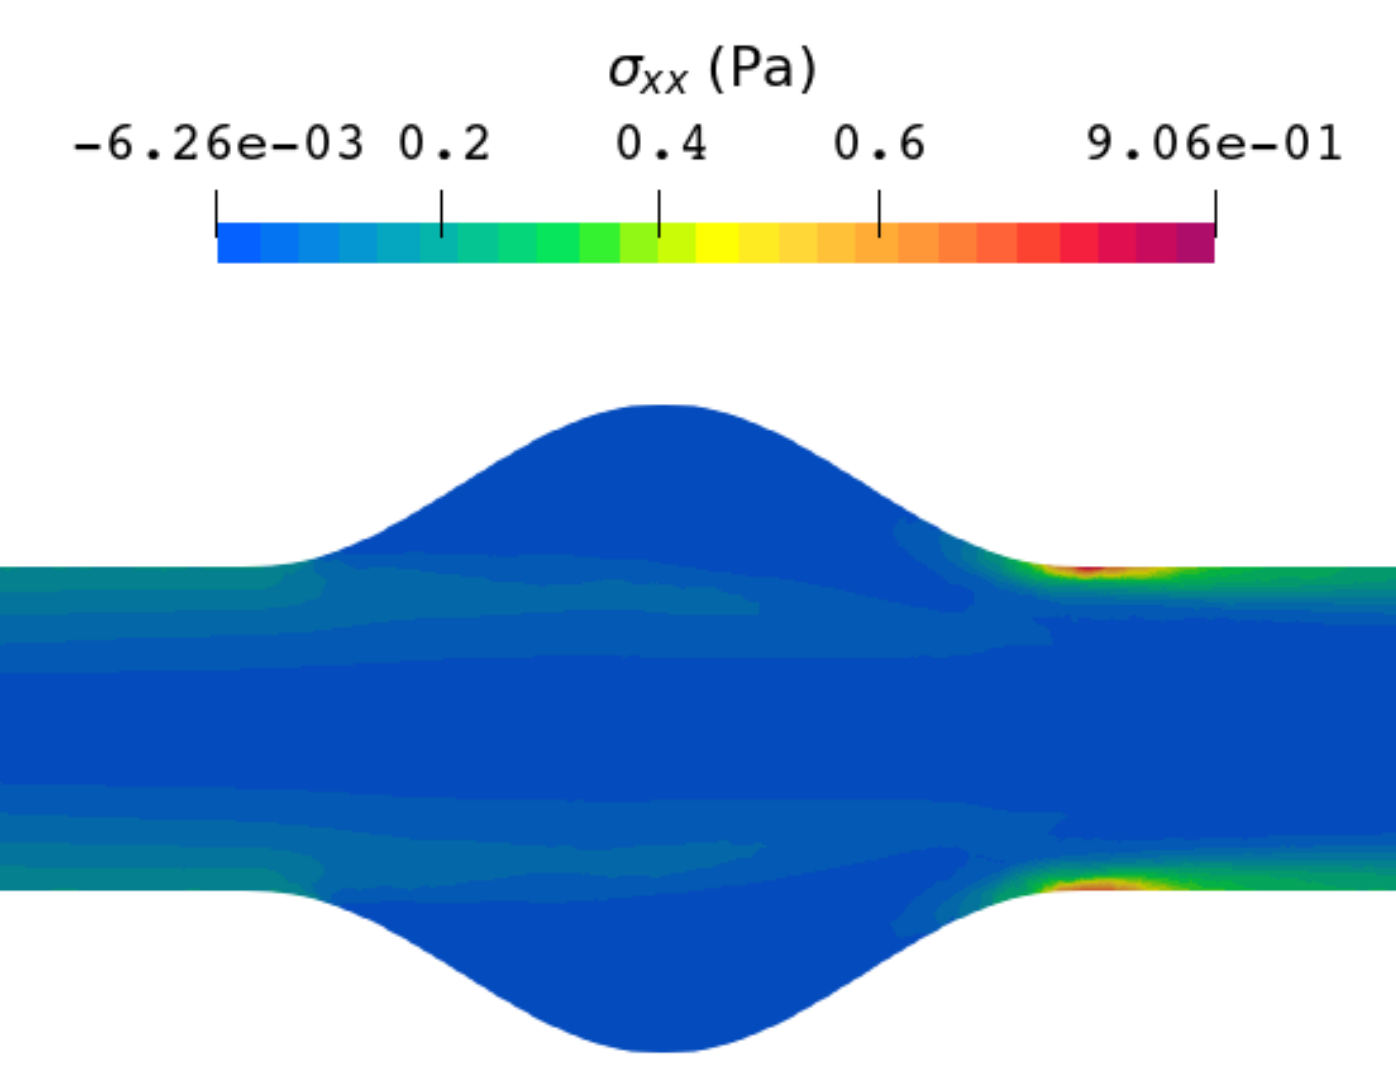
\includegraphics[scale=0.49]{Figures_aneurism/stressXX_viscoelastic.png} \label{fig:aneurysm_stress_viscoelastic}}
    \caption{First component of the stresses. Comparison between Newtonian and viscoelastic regimes in a fluid domain transversal cut.}
    \label{fig:aneurysm_comparison_viscoelastic}
\end{figure}

\begin{figure}[h!]
    \centering
    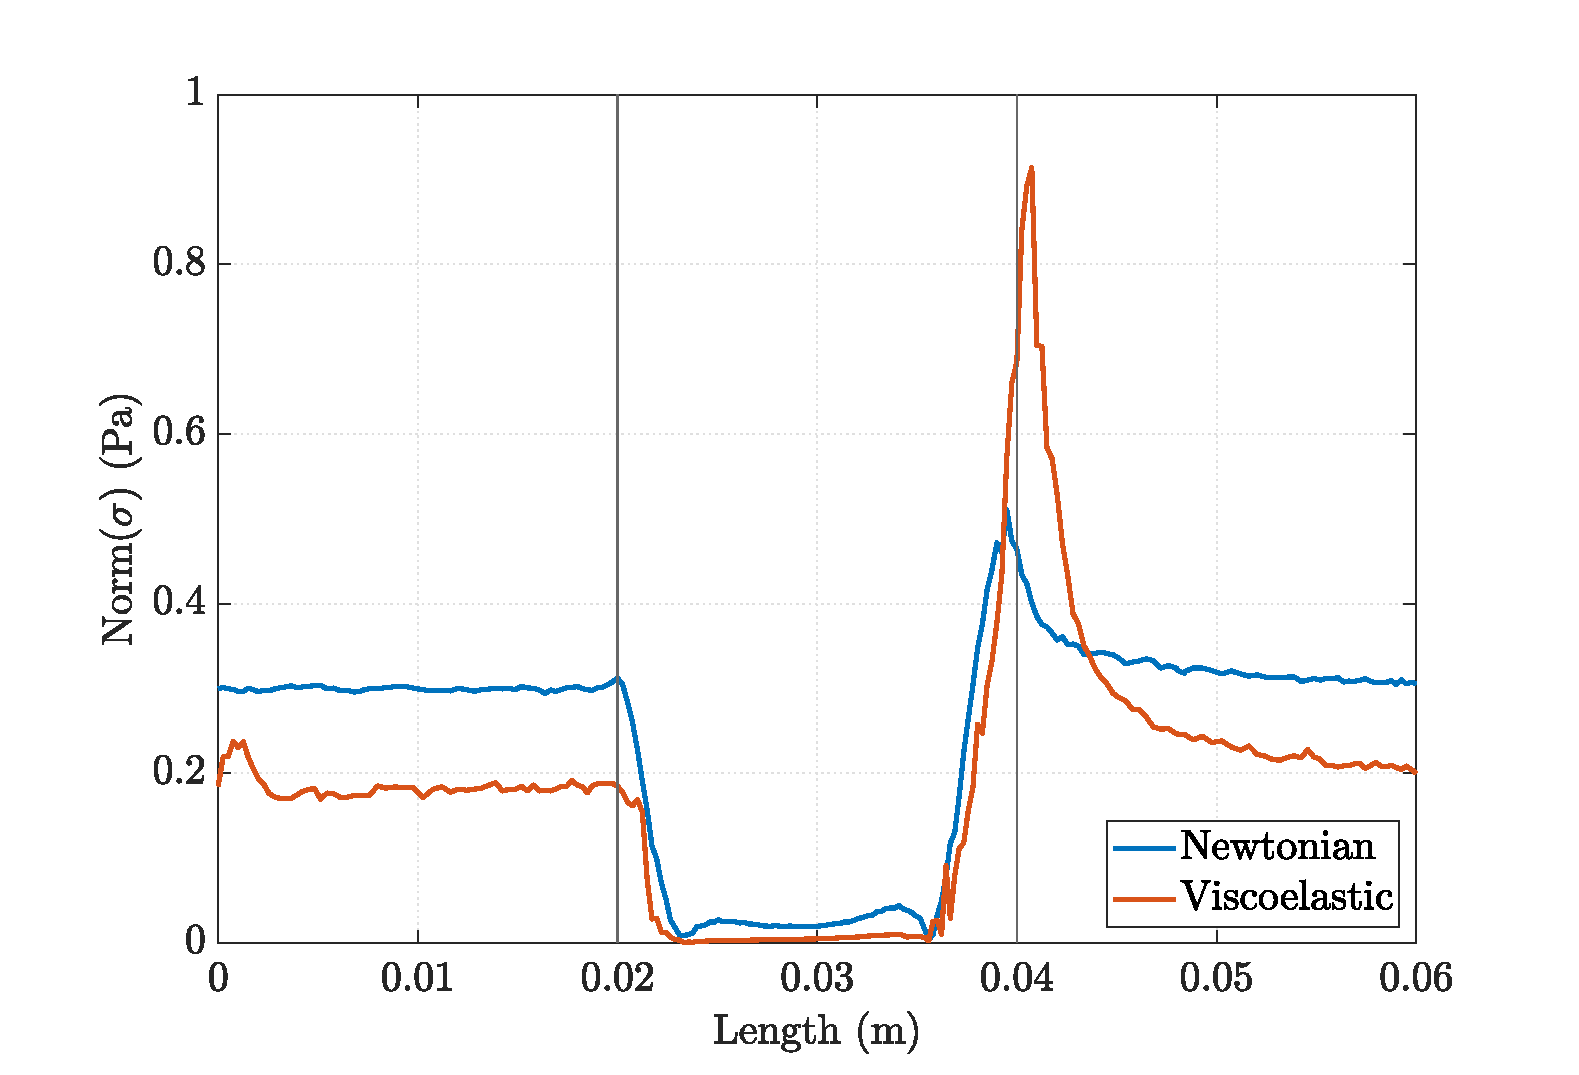
\includegraphics[scale=0.5]{Figures_aneurism/Norm_stresses.eps}
    \caption{Comparison for the stress norm along the top wall in the plane $z=0$ of the fluid domain.}
    \label{fig:aneurysm_norm}
\end{figure}


%%%%%%%%%%%%%%%%%%%%%%%%%%%%%%%%%%%%%%%
%
% CONCLUSIONS
%
%%%%%%%%%%%%%%%%%%%%%%%%%%%%%%%%%%%%%%

\section{Conclusions} \label{sec:conclusions}

In this work, a numerical approximation for VFSI problems with viscoelastic fluids in which elasticity can be dominant has been presented. The main idea is to reproduce scenarios with a viscoelastic fluid model and particularly using the so-called log-conformation reformulation. This technique allows to treat the exponential growth of the elastic stresses and, therefore, extend the range of Weissenberg numbers in which the VFSI problem can be solved.

Several numerical examples have been run to assess the performance of the proposed VFSI problem and its applicability to viscoelastic flows with high elasticity. First of all, some examples with Newtonian fluids have been performed to validate our FSI model and to show that both the standard and the logarithmic formulation presented in Section \ref{sec:Viscoelastic-fluid-flow-prob} match with the classical Navier-Stokes equations written in a three-field setting when ${\rm We}=0$.

Regarding the elasticity of the fluid, we have shown the effect of increasing it. When elasticity increases, stresses do so significantly. This effect causes elastic forces to grow up and, therefore, fluid tractions on the solid become higher. 

With regards to the three-field formulations presented in this work, several conclusions can be drawn. Firstly, we have shown the effect of considering the stress as a primary unknown. It becomes crucial when dealing with viscoelastic flows due to the need to solve an additional differential equation for the stresses. Furthermore, more accurate results are obtained for stresses with respect to the classical two-field formulation in which these stresses are computed as a post-process. This is clearly a benefit when computing fluid tractions to be imposed in the solid problem. When facing high elasticity cases for the same mesh, the standard formulation fails to obtain smooth solutions, whereas the logarithmic formulation is able to handle these situations and regular solutions are obtained.

To end up, we have demonstrated the good performance of our implementation in a 3D problem. Furthermore, the effect of considering the blood flow as a viscoelastic fluid and to mimic the arteries as hyperelastic materials has been studied. The results prove that differences between Newtonian and viscoelastic models should not be underestimated and that viscoelastic constitutive modeling is necessary, specially when the flow rate in the artery increases.

\section*{Declaration of competing interest}

The authors declare that they have no known competing financial interests or personal relationships that could have appeared to influence the work reported in this paper.

\section*{Acknowledgements}

L. Moreno acknowledges the support received from the project Nemesis, LARE\_BIRD2020\_01 (id: 33593). I. Casta\~nar gratefully acknowledges the support received from the Ag\`encia de Gesti\'o d'Ajuts i de Recerca through the predoctoral FI grant 2019-FI-B-00649. R. Codina gratefully acknowledges the support received through the ICREA Acad\`emia Research Program of the Catalan Government. This work was partially funded through the TOP-FSI: RTI2018-098276-B-I00 project of the Spanish Government. CIMNE is a recipient of a ``Severo Ochoa Programme for Centers of Excellence in R\&D'' grant (CEX2018-000797-S) by the Spanish Ministry of Economy and Competitiveness.
               
%\nocite{*}     
\bibliographystyle{unsrt}
\bibliography{bibliography.bib}

\end{document}